%% LyX 2.4.3 created this file.  For more info, see https://www.lyx.org/.
%% Do not edit unless you really know what you are doing.
\documentclass[journal,article,submit,pdftex,moreauthors]{Definitions/mdpi}
\usepackage{textcomp}
\usepackage[utf8]{inputenc}
\usepackage{longtable}
\usepackage{float}
\usepackage{url}
\usepackage{pdflscape}
\usepackage{amsbsy}
\usepackage{amstext}
\usepackage{graphicx}

\makeatletter

%%%%%%%%%%%%%%%%%%%%%%%%%%%%%% LyX specific LaTeX commands.

\Title{A Novel Weather-Aware Irrigation Scheduling Benchmark for Continuous
Global Optimization}

\TitleCitation{A Novel Weather-Aware Irrigation Scheduling Benchmark for Continuous
Global Optimization}

\Author{Vasileios Charilogis$^{1}$, Ioannis G. Tsoulos$^{2,*}$, Gianni Anna
Maria$^{3}$ and Dimitrios Tsalikakis$^{4}$}

\AuthorNames{Vasileios Charilogis, Ioannis G. Tsoulos, Gianni Anna Maria and Dimitrios
Tsalikakis.}

\AuthorCitation{Charilogis, V. , Tsoulos, I.G. , Gianni, A. M, Tsalikakis, D.}


\address{$^{1}$\quad{}Department of Informatics and Telecommunications,
University of Ioannina, 47150 Kostaki Artas, Greece, v.charilog@uoi.gr\\
$^{2}$\quad{}Department of Informatics and Telecommunications, University
of Ioannina, 47150 Kostaki Artas, Greece, itsoulos@uoi.gr\\
$^{3}$\quad{}Department of Informatics and Telecommunications, University
of Ioannina, 47150 Kostaki Artas, Greece, am.gianni@uoi.gr\\
$^{4}$\quad{}Department of Engineering Informatics and Telecommunications,
University of Western Macedonia, 50100 Kozani, Greece, dtsalikakis@uowm.gr}


\corres{Correspondence: itsoulos@uoi.gr}


\abstract{This article presents a new literature-informed benchmark problem
for continuous global optimization, inspired by the semantics of weather-aware
irrigation scheduling. The problem is formulated as a continuous minimization
task in which irrigation decisions are determined under synthetically
generated but agronomically motivated weather-dependent water demand,
rainfall effects, and nonlinear operational penalties. The proposed
benchmark is intentionally synthetic and self-contained requiring
no external datasets or field-calibrated parameters while its components
are grounded in established concepts from irrigation science such
as evapotranspiration-based demand estimation, yield-response-to-water
relationships, and weather-dependent scheduling principles. It is
designed to be sufficiently challenging for numerical optimization
while retaining a clear agronomic interpretation. The article provides
the full mathematical formulation of the problem, explains its main
components and parameters, and reports an experimental study focused
on its optimization behavior using eight established continuous optimizers
across five problem dimensions. From this perspective, the proposed
problem is positioned within a clear framework for the study of real-world-inspired
continuous optimization benchmarks, offering an additional case in
which mathematical formulation, practical interpretation, and experimental
investigation coexist in a coherent and systematic manner.}


\keyword{continuous global optimization; benchmark problems; real-world optimization;
irrigation scheduling; weather-aware optimization; black-box optimization;
non-separable objective functions}

\newcommand*\LyXZeroWidthSpace{\hspace{0pt}}
\DeclareTextSymbolDefault{\textquotedbl}{T1}
%% Because html converters don't know tabularnewline
\providecommand{\tabularnewline}{\\}

%%%%%%%%%%%%%%%%%%%%%%%%%%%%%% User specified LaTeX commands.
\usepackage{rotating}

%  LaTeX support: latex@mdpi.com 
%  For support, please attach all files needed for compiling as well as the log file, and specify your operating system, LaTeX version, and LaTeX editor.

%=================================================================


% For posting an early version of this manuscript as a preprint, you may use "preprints" as the journal and change "submit" to "accept". The document class line would be, e.g., \documentclass[preprints,article,accept,moreauthors,pdftex]{mdpi}. This is especially recommended for submission to arXiv, where line numbers should be removed before posting. For preprints.org, the editorial staff will make this change immediately prior to posting.

%--------------------
% Class Options:
%--------------------
%----------
% journal
%----------
% Choose between the following MDPI journals:
% acoustics, actuators, addictions, admsci, adolescents, aerospace, agriculture, agriengineering, agronomy, ai, algorithms, allergies, alloys, analytica, animals, antibiotics, antibodies, antioxidants, applbiosci, appliedchem, appliedmath, applmech, applmicrobiol, applnano, applsci, aquacj, architecture, arts, asc, asi, astronomy, atmosphere, atoms, audiolres, automation, axioms, bacteria, batteries, bdcc, behavsci, beverages, biochem, bioengineering, biologics, biology, biomass, biomechanics, biomed, biomedicines, biomedinformatics, biomimetics, biomolecules, biophysica, biosensors, biotech, birds, bloods, blsf, brainsci, breath, buildings, businesses, cancers, carbon, cardiogenetics, catalysts, cells, ceramics, challenges, chemengineering, chemistry, chemosensors, chemproc, children, chips, cimb, civileng, cleantechnol, climate, clinpract, clockssleep, cmd, coasts, coatings, colloids, colorants, commodities, compounds, computation, computers, condensedmatter, conservation, constrmater, cosmetics, covid, crops, cryptography, crystals, csmf, ctn, curroncol, currophthalmol, cyber, dairy, data, dentistry, dermato, dermatopathology, designs, diabetology, diagnostics, dietetics, digital, disabilities, diseases, diversity, dna, drones, dynamics, earth, ebj, ecologies, econometrics, economies, education, ejihpe, electricity, electrochem, electronicmat, electronics, encyclopedia, endocrines, energies, eng, engproc, ent, entomology, entropy, environments, environsciproc, epidemiologia, epigenomes, est, fermentation, fibers, fintech, fire, fishes, fluids, foods, forecasting, forensicsci, forests, foundations, fractalfract, fuels, futureinternet, futureparasites, futurepharmacol, futurephys, futuretransp, galaxies, games, gases, gastroent, gastrointestdisord, gels, genealogy, genes, geographies, geohazards, geomatics, geosciences, geotechnics, geriatrics, hazardousmatters, healthcare, hearts, hemato, heritage, highthroughput, histories, horticulturae, humanities, humans, hydrobiology, hydrogen, hydrology, hygiene, idr, ijerph, ijfs, ijgi, ijms, ijns, ijtm, ijtpp, immuno, informatics, information, infrastructures, inorganics, insects, instruments, inventions, iot, j, jal, jcdd, jcm, jcp, jcs, jdb, jeta, jfb, jfmk, jimaging, jintelligence, jlpea, jmmp, jmp, jmse, jne, jnt, jof, joitmc, jor, journalmedia, jox, jpm, jrfm, jsan, jtaer, jzbg, kidney, kidneydial, knowledge, land, languages, laws, life, liquids, literature, livers, logics, logistics, lubricants, lymphatics, machines, macromol, magnetism, magnetochemistry, make, marinedrugs, materials, materproc, mathematics, mca, measurements, medicina, medicines, medsci, membranes, merits, metabolites, metals, meteorology, methane, metrology, micro, microarrays, microbiolres, micromachines, microorganisms, microplastics, minerals, mining, modelling, molbank, molecules, mps, msf, mti, muscles, nanoenergyadv, nanomanufacturing, nanomaterials, ncrna, network, neuroglia, neurolint, neurosci, nitrogen, notspecified, nri, nursrep, nutraceuticals, nutrients, obesities, oceans, ohbm, onco, oncopathology, optics, oral, organics, organoids, osteology, oxygen, parasites, parasitologia, particles, pathogens, pathophysiology, pediatrrep, pharmaceuticals, pharmaceutics, pharmacoepidemiology, pharmacy, philosophies, photochem, photonics, phycology, physchem, physics, physiologia, plants, plasma, pollutants, polymers, polysaccharides, poultry, powders, preprints, proceedings, processes, prosthesis, proteomes, psf, psych, psychiatryint, psychoactives, publications, quantumrep, quaternary, qubs, radiation, reactions, recycling, regeneration, religions, remotesensing, reports, reprodmed, resources, rheumato, risks, robotics, ruminants, safety, sci, scipharm, seeds, sensors, separations, sexes, signals, sinusitis, skins, smartcities, sna, societies, socsci, software, soilsystems, solar, solids, sports, standards, stats, stresses, surfaces, surgeries, suschem, sustainability, symmetry, synbio, systems, taxonomy, technologies, telecom, test, textiles, thalassrep, thermo, tomography, tourismhosp, toxics, toxins, transplantology, transportation, traumacare, traumas, tropicalmed, universe, urbansci, uro, vaccines, vehicles, venereology, vetsci, vibration, viruses, vision, waste, water, wem, wevj, wind, women, world, youth, zoonoticdis 

%---------
% article
%---------
% The default type of manuscript is "article", but can be replaced by: 
% abstract, addendum, article, book, bookreview, briefreport, casereport, comment, commentary, communication, conferenceproceedings, correction, conferencereport, entry, expressionofconcern, extendedabstract, datadescriptor, editorial, essay, erratum, hypothesis, interestingimage, obituary, opinion, projectreport, reply, retraction, review, perspective, protocol, shortnote, studyprotocol, systematicreview, supfile, technicalnote, viewpoint, guidelines, registeredreport, tutorial
% supfile = supplementary materials

%----------
% submit
%----------
% The class option "submit" will be changed to "accept" by the Editorial Office when the paper is accepted. This will only make changes to the frontpage (e.g., the logo of the journal will get visible), the headings, and the copyright information. Also, line numbering will be removed. Journal info and pagination for accepted papers will also be assigned by the Editorial Office.

%------------------
% moreauthors
%------------------
% If there is only one author the class option oneauthor should be used. Otherwise use the class option moreauthors.

%---------
% pdftex
%---------
% The option pdftex is for use with pdfLaTeX. If eps figures are used, remove the option pdftex and use LaTeX and dvi2pdf.

%=================================================================
% MDPI internal commands - do not modify
\firstpage{1} 
 
\setcounter{page}{\@firstpage} 

\pubvolume{1}
\issuenum{1}
\articlenumber{0}
\pubyear{2024}
\copyrightyear{2024}
%\externaleditor{Academic Editor: Firstname Lastname} % For journal Automation, please change Academic Editor to "Communicated by"
\datereceived{}
\daterevised{ } % Comment out if no revised date
\dateaccepted{}
\datepublished{}
%\datecorrected{} % Corrected papers include a "Corrected: XXX" date in the original paper.
%\dateretracted{} % Corrected papers include a "Retracted: XXX" date in the original paper.
\hreflink{} % If needed use \linebreak
%\doinum{}
%------------------------------------------------------------------
% The following line should be uncommented if the LaTeX file is uploaded to arXiv.org
%\pdfoutput=1

%=================================================================
% Add packages and commands here. The following packages are loaded in our class file: fontenc, inputenc, calc, indentfirst, fancyhdr, graphicx, epstopdf, lastpage, ifthen, lineno, float, amsmath, setspace, enumitem, mathpazo, booktabs, titlesec, etoolbox, tabto, xcolor, soul, multirow, microtype, tikz, totcount, changepage, attrib, upgreek, cleveref, amsthm, hyphenat, natbib, hyperref, footmisc, url, geometry, newfloat, caption

%=================================================================
%% Please use the following mathematics environments: Theorem, Lemma, Corollary, Proposition, Characterization, Property, Problem, Example, ExamplesandDefinitions, Hypothesis, Remark, Definition, Notation, Assumption
%% For proofs, please use the proof environment (the amsthm package is loaded by the MDPI class).

%=================================================================
% The fields PACS, MSC, and JEL may be left empty or commented out if not applicable
%\PACS{J0101}
%\MSC{}
%\JEL{}

%%%%%%%%%%%%%%%%%%%%%%%%%%%%%%%%%%%%%%%%%%
% Only for the journal Diversity
%\LSID{\url{http://}}

%%%%%%%%%%%%%%%%%%%%%%%%%%%%%%%%%%%%%%%%%%
% Only for the journal Applied Sciences:
%\featuredapplication{Authors are encouraged to provide a concise description of the specific application or a potential application of the work. This section is not mandatory.}
%%%%%%%%%%%%%%%%%%%%%%%%%%%%%%%%%%%%%%%%%%

%%%%%%%%%%%%%%%%%%%%%%%%%%%%%%%%%%%%%%%%%%
% Only for the journal Data:
%\dataset{DOI number or link to the deposited data set in cases where the data set is published or set to be published separately. If the data set is submitted and will be published as a supplement to this paper in the journal Data, this field will be filled by the editors of the journal. In this case, please make sure to submit the data set as a supplement when entering your manuscript into our manuscript editorial system.}

%\datasetlicense{license under which the data set is made available (CC0, CC-BY, CC-BY-SA, CC-BY-NC, etc.)}

%%%%%%%%%%%%%%%%%%%%%%%%%%%%%%%%%%%%%%%%%%
% Only for the journal Toxins
%\keycontribution{The breakthroughs or highlights of the manuscript. Authors can write one or two sentences to describe the most important part of the paper.}

%%%%%%%%%%%%%%%%%%%%%%%%%%%%%%%%%%%%%%%%%%
% Only for the journal Encyclopedia
%\encyclopediadef{Instead of the abstract}
%\entrylink{The Link to this entry published on the encyclopedia platform.}
%%%%%%%%%%%%%%%%%%%%%%%%%%%%%%%%%%%%%%%%%%

%%%%%%%%%%%%%%%%%%%%%%%%%%%%%%%%%%%%%%%%%%
% Only for the journal Advances in Respiratory Medicine
%\addhighlights{yes}
%\renewcommand{\addhighlights}{%

%\noindent This is an obligatory section in “Advances in Respiratory Medicine”, whose goal is to increase the discoverability and readability of the article via search engines and other scholars. Highlights should not be a copy of the abstract, but a simple text allowing the reader to quickly and simplified find out what the article is about and what can be cited from it. Each of these parts should be devoted up to 2~bullet points.\vspace{3pt}\\
%\textbf{What are the main findings?}
% \begin{itemize}[labelsep=2.5mm,topsep=-3pt]
% \item First bullet.
% \item Second bullet.
% \end{itemize}\vspace{3pt}
%\textbf{What is the implication of the main finding?}
% \begin{itemize}[labelsep=2.5mm,topsep=-3pt]
% \item First bullet.
% \item Second bullet.
% \end{itemize}
%}
%%%%%%%%%%%%%%%%%%%%%%%%%%%%%%%%%%%%%%%%%%
% Added by lyx2lyx
\usepackage{array}
\usepackage[noend]{algpseudocode}
\algrenewcommand\algorithmicindent{1.0em}

\makeatother

\begin{document}
\maketitle

\section{Introduction\label{sec:Introduction}}

Optimization plays a central role in science and engineering because
many practical decision problems can be formulated as the search for
variable configurations that minimize cost, maximize performance,
or satisfy multiple competing operational criteria. In continuous
settings, the resulting problems are often nonlinear, multimodal,
nonconvex, and derivative-free, which makes the empirical study of
optimization algorithms strongly dependent on the availability of
representative benchmark problems \citep{Rios}. Population-based
and nature-inspired metaheuristics including differential evolution,
particle swarm optimization, evolution strategies, and ant colony
optimization have demonstrated broad competence on such problems,
yet their comparative evaluation remains a persistent methodological
challenge \citep{Sharma}, \citep{Mohamed}. In the absence of systematic
benchmarking, performance claims are frequently overstated, algorithm
rankings are unstable across problem classes, and the generalizable
strengths and weaknesses of competing methods remain obscured \citep{Naser},
\citep{Kudela}.

Benchmark design is therefore not a peripheral issue but a methodological
one. The two dominant paradigms for continuous benchmarking the Congress
on Evolutionary Computation (CEC) suites and the Black-Box Optimization
Benchmarking (BBOB) platform have each contributed important infrastructure
for controlled algorithm comparison \citep{Liang-1}, \citep{Hansen-1}.
CEC suites, including CEC 2014, CEC 2017, CEC 2021, and CEC 2022,
provide fixed-budget comparisons on shifted, rotated, and hybridized
analytical functions across multiple dimensionalities \citep{Awad}.
BBOB, developed within the COCO platform, adopts a target-based approach
and covers a set of 24 single-objective functions with documented
landscape properties, recently extended to large-scale dimensions
up to 640 \citep{Varelas}. Both platforms have made substantial contributions
to reproducible benchmarking, and recent comprehensive reviews have
catalogued several hundred test functions in use across the optimization
literature \citep{Sharma}, \citep{Jamil}. At the same time, recent
analyses have shown that the choice of benchmark problems can substantially
alter empirical conclusions: algorithms that rank highly on CEC 2020
often perform poorly on CEC 2014 and CEC 2017, and vice versa \citep{Naser},
\citep{Kudela}, \citep{Piotrowski-1}. The number of allowed function
evaluations further modulates rankings, suggesting that no single
benchmark configuration provides a definitive ordering of optimizers
\citep{Piotrowski-1}. These findings reinforce the need for diverse,
independently designed benchmark problems whose difficulty structure
is transparent and whose components can be subjected to controlled
ablation. Recent critical analyses have further emphasized that algorithm
rankings are highly sensitive to the specific benchmark suite employed
\citep{Kudela,Piotrowski}, and comprehensive surveys have catalogued
the structural properties including separability, modality, and conditioning
that distinguish existing test functions from one another \citep{Kumar}.
These findings underscore the value of introducing new benchmarks
whose difficulty mechanisms are independently documented and whose
landscape properties differ qualitatively from those of existing suites.

A complementary body of work has emphasized the value of real-world
inspired benchmark problems, whose objective structures reflect realistic
coupling, delayed effects, threshold mechanisms, and non-separable
stage interactions that are rarely present in purely analytical test
functions \citep{Naser}, \citep{Kudela}, \citep{Sharma}. The IEEE
CEC 2011 competition introduced a set of practical optimization problems
drawn from engineering domains, and subsequent efforts have proposed
test suites for constrained, large-scale, and multi-objective problems
motivated by physical or operational constraints \citep{Das}. Recent
large-scale benchmarks have additionally highlighted the importance
of heterogeneous module coupling and non-uniform interaction patterns,
features that are genuinely present in physical systems but largely
absent from classic analytical suites \citep{Li}. The methodological
literature has accordingly called for benchmarks that combine interpretability
so that the source of difficulty can be understood and communicated
with sufficient computational challenge to stress modern population-based
solvers across a range of dimensionalities \citep{Naser}, \citep{Sharma},
\citep{Jamil}.

Within agricultural water management, irrigation scheduling provides
a natural domain for such benchmark construction. Agriculture accounts
for approximately 70 percent of global freshwater withdrawals, and
the efficient allocation of irrigation water across a growing season
has direct implications for food production, resource conservation,
and economic viability \citep{Jamal}. Existing studies have investigated
evapotranspiration-driven scheduling based on the FAO Penman-Monteith
framework, weather-aware irrigation control using probabilistic forecast
integration, and simulation-optimization frameworks that couple crop
growth models with operational decision support \citep{Allen}, \citep{Doorenbos},
\citep{Wang}. Real-time and data-assimilation-based scheduling approaches
have demonstrated that incorporating short-term weather forecasts
and sensor observations into the decision loop can substantially improve
water use efficiency relative to rule-based alternatives \citep{Linker},
\citep{Li-1}. Systematic reviews of simulation-optimization methods
for irrigation scheduling have further shown that the choice of crop
model, objective function structure, and optimization algorithm interacts
in complex ways, highlighting the need for reproducible and well-characterized
problem formulations \citep{Zhao}. However, many available formulations
are developed as calibrated management tools for specific field conditions
and crop systems rather than as intentionally difficult black-box
benchmarks for continuous global optimization. Their calibration to
site-specific agronomic data makes them neither self-contained nor
algorithmically transparent, limiting their utility as general-purpose
benchmarks. At the same time, the standard analytical benchmark suites
used in continuous optimization, including CEC and BBOB, lack the
semantic interpretability, state-dependent coupling, and operational
realism that physically motivated domains such as irrigation scheduling
naturally provide. There is therefore a recognized gap for benchmark
problems that are simultaneously self-contained and analytically transparent,
yet exhibit the non-separable, stateful, and rugged landscape structure
that arises in real operational systems.

The present article therefore introduces a new literature-informed
weather-coupled irrigation scheduling benchmark whose explicit role
is not to reproduce a field-calibrated agronomic model, but to provide
a mathematically explicit, semantically meaningful, and computationally
demanding optimization landscape that bridges the gap identified above.
The benchmark is entirely synthetic and deterministic: all exogenous
weather and crop profiles are generated analytically from a normalized
stage coordinate, and no external datasets, site-specific calibration,
or field measurements are required. At the same time, its components
are grounded in established agronomic concepts: evapotranspiration-based
demand estimation following the FAO framework \citep{Allen}, yield-response-to-water
relationships consistent with the classical model of Doorenbos and
Kassam \citep{Doorenbos}, and weather-dependent scheduling principles
as discussed in \citep{Wang}. As a result, every term in the objective
function retains a clear physical interpretation, even though the
benchmark itself is not a digital twin of any specific field or crop
system. The proposed benchmark is fully deterministic and analytically
self-contained: all exogenous weather and crop profiles are generated
from a normalized stage coordinate, requiring no external datasets,
calibrated parameters, or field-specific inputs. Its objective function
deliberately integrates six distinct difficulty mechanisms recursive
soil-water storage propagation, oscillatory irrigation efficiency
modulation, threshold-triggered drainage losses, multiplicative seasonal
yield aggregation, neighbor-coupled hydraulic load, and a deceptive
preferred-window penalty each of which has a clear agronomic interpretation
and a quantifiable contribution to search landscape ruggedness. The
benchmark is therefore positioned at the intersection of two research
communities: it retains the domain semantics and operational realism
of agricultural water management while providing the analytical transparency,
controlled difficulty structure, and scalable dimensionality that
the continuous optimization community requires for rigorous algorithm
comparison.

The remainder of the article is organized as follows. Section \ref{sec:WeatherProblem}
presents the proposed benchmark, including its background \ref{subsec:Background},
full mathematical formulation \ref{subsec:Formulation}, and experimental
behavior \ref{subsec:ExpResults} under a common evaluation setting
\ref{subsec:ExpProtocol}. Section \ref{sec:Discussion} discusses
the optimization signature of the problem from a problem-centered
perspective, and Section \ref{sec:conclusions} summarizes the main
conclusions.

\section{Weather-Coupled Irrigation Scheduling Benchmark\label{sec:WeatherProblem}}

\subsection{Background of the Problem\label{subsec:Background}}

The proposed benchmark is motivated by the need to represent irrigation
scheduling as a genuinely coupled seasonal decision process rather
than as a separable stage-wise water allocation rule. In realistic
irrigation environments, the amount of water applied at one stage
influences not only the immediate water balance of the crop, but also
subsequent storage, drainage, evaporative losses, and the cumulative
preservation of seasonal productivity \citep{Allen,Doorenbos,Wang,Linker,Li,Zhao}.
This makes the domain naturally suitable for benchmark construction
aimed at non-separable and state-dependent continuous optimization.

The benchmark is intentionally synthetic in the sense that all exogenous
profiles are generated analytically from the normalized stage coordinate,
yet it remains literature-informed in its semantic structure. To make
this grounding explicit, the following correspondences between benchmark
components and agronomic concepts are noted. The stage-wise crop evapotranspiration
demand $ETc_{i}=ETo_{i}\cdot Kc_{i}\cdot\Delta t$ follows the standard
reference-evapotranspiration construction of the FAO Penman Monteith
framework \citep{Allen}, in which a reference atmospheric demand
$ETo$ is scaled by a crop-specific coefficient Kc to obtain actual
crop water requirements. The multiplicative yield-preservation factor
$Y_{rel}=\prod y_{i}$ is consistent with the classical yield-response-to-water
model of Doorenbos and Kassam \citep{Doorenbos}, which relates relative
yield reduction to relative evapotranspiration deficit through a crop-specific
sensitivity coefficient $Ky$. The recursive soil-water storage transition
$S_{i+1}=f(S_{i},rain_{i},I_{i}^{eff},...)$ reflects the widely adopted
soil water-balance approach used in simulation-optimization frameworks
for irrigation scheduling \citep{Linker,Li-1,Zhao}, in which the
storage state at each stage depends on incoming water, drainage, and
evaporative losses from the preceding stage. The weather-dependent
profiles for heat, wind, rainfall, and tariff represent stylized seasonal
patterns that capture the qualitative behavior documented in weather-aware
scheduling studies \citep{Jamal,Wang}, although their specific functional
forms are chosen for analytical convenience rather than site-specific
fidelity.

Beyond these literature-informed components, additional oscillatory,
thresholded, and deceptive mechanisms are deliberately embedded to
produce a challenging optimization landscape. These include the oscillatory
modulation of irrigation efficiency $\eta_{i}(x)$, which generates
repeated local attraction basins, the threshold-triggered deep drainage
loss, which introduces nonsmooth regime changes, and the deceptive
preferred-window penalty $P_{win}$, which attracts solvers toward
irrigation levels that are suboptimal under the full objective. These
mechanisms are synthetic ruggedness generators with no claim to precise
field physics, they are introduced to make the benchmark genuinely
difficult for modern continuous optimizers while remaining structurally
interpretable. As a result, the problem should be interpreted as a
literature-informed optimization benchmark with agronomic meaning,
not as a calibrated digital twin of a particular field or crop system.\textquotedbl{}

\subsection{Mathematical Formulation\label{subsec:Formulation}}

Let $D\geq4$ denote the problem dimension, and let$\boldsymbol{x}=(x_{1},x_{2},\ldots,x_{D})^{\mathsf{T}}$
be the decision vector, where$x_{i}$ is the irrigation depth (mm)
applied at stage $i$ of a synthetic growing season. The feasible
set is the hyper-rectangle
\[
\Omega=[0,80]^{D},\qquad0\leq x_{i}\leq80,\qquad i=1,\ldots,D.
\]

The only hard constraints imposed on the problem are the box bounds
$0\leq x_{i}\leq80$ on the decision variables. The internal storage
state $S_{i}$\LyXZeroWidthSpace{} is maintained within admissible
bounds $[0,\,S_{i}^{max}]$ through the clipping operator in the storage
transition equation, which acts as an implicit state constraint enforced
by construction rather than by external penalization. All remaining
operational constraints are treated as soft penalties incorporated
directly into the objective function: the seasonal water budget is
softly constrained through $P_{budget}$\LyXZeroWidthSpace , which
penalizes deviation from the target $B_{D}=28D$, peak hydraulic demand
is softly constrained through $P_{peak}$ and terminal storage is
regularized through $P_{term}$\LyXZeroWidthSpace . This soft-constraint
formulation is deliberate, as it preserves the box-constrained structure
of the search domain while embedding operational feasibility requirements
into the landscape topology of the objective.

The season length is fixed at $120$ days, so the stage duration is
\[
\Delta t=\frac{120}{D},
\]
 and the normalized stage coordinate is
\[
s_{i}=\frac{i}{D+1},\qquad i=1,\ldots,D.
\]
 Recommended difficult dimensions are $D\in\{24,30,50,70,100\}$,
with $D=24$ and $D=30$ suitable for routine experiments and $D=50$
or $D=70$ or $D=100$ producing substantially harder landscapes for
population-based optimizers.

To make the benchmark fully deterministic and self-contained, all
exogenous weather and crop coefficients are generated analytically
from the normalized stage coordinate $s_{i}$\LyXZeroWidthSpace .
No stochastic, scenario-based, or externally sampled weather realizations
are involved: every weather profile is a fixed, closed-form trigonometric
function of $s_{i}$ that produces identical values for any given
dimension $D$. This design choice eliminates all sources of exogenous
randomness from the benchmark, ensuring that any variability in optimization
outcomes is attributable solely to the stochastic search process of
the optimizer and not to weather input uncertainty. The specific functional
forms are chosen to reproduce qualitative seasonal patterns (e.g.,
mid-season peaks in temperature and evapotranspiration, early-season
dominance of rainfall) that are consistent with the general behavior
documented in weather-aware scheduling studies \citep{Jamal,Wang},
although they do not represent any particular geographic location
or climate record. The stage-wise profiles are defined as:
\[
ETo_{i}=2.8+3.2\sin^{2}(\pi s_{i}),
\]
\[
Kc_{i}=0.55+0.65\sin(\pi s_{i}),
\]
\[
rain_{i}=8+18\cos^{2}(\pi s_{i}),
\]
\[
Ky_{i}=0.85+0.55\sin(\pi s_{i}),
\]
\[
heat_{i}=0.40+0.60\sin^{2}(\pi s_{i}),
\]
\[
wind_{i}=0.35+0.65\cos^{2}(\pi s_{i}),
\]
\[
tariff_{i}=0.90+0.18\sin(2\pi s_{i}+0.20),
\]
\[
\eta_{base,i}=0.78+0.10\cos(\pi s_{i}),
\]
\[
\rho_{i}=0.52+0.18\sin^{2}(\pi s_{i}),
\]
\[
S_{i}^{max}=50+20\sin^{2}(\pi s_{i}),
\]
\[
freq_{i}=0.22+0.09\sin(\pi s_{i}),
\]
 and
\[
\phi_{i}=0.70i+0.30\sin(2\pi s_{i}).
\]
 The crop evapotranspiration demand follows the standard evapotranspiration-based
construction
\[
ETc_{i}=ETo_{i}Kc_{i}\Delta t,
\]
 which grounds the benchmark in classical irrigation science \citep{Naser}.
The coefficient $Ky_{i}$ is used as a stage sensitivity factor in
the relative yield-preservation component, consistent with the general
idea of yield response to water stress \citep{Doorenbos}.

The first major source of difficulty is local decision coupling. A
neighbor-coupled hydraulic load is introduced as
\[
N_{i}=0.60x_{i}+0.25x_{i-1}+0.15x_{i+1},
\]
 with boundary conventions $x_{0}=x_{D+1}=0$. Effective irrigation
efficiency is then defined by the oscillatory nonlinear law
\[
\eta_{i}(\boldsymbol{x})=\eta_{base,i}\Big[1-0.22\sin^{2}(freq_{i}x_{i}+\phi_{i})-0.10\sin^{2}(0.07N_{i}+0.50\phi_{i})\Big],
\]
 clipped to the interval $[0.45,1.00]$, and the effective irrigation
becomes
\[
I_{i}^{eff}=\eta_{i}(\boldsymbol{x})x_{i}.
\]
 These oscillatory factors are synthetic ruggedness generators. They
are not intended to claim precise field physics, they are introduced
to generate repeated attraction basins and to make coordinate-wise
search substantially less effective.

The second major source of difficulty is path dependence through a
synthetic soil-water storage state $S_{i}$. The initial storage is
fixed by
\[
S_{1}=0.35S_{1}^{max}.
\]
 The total water available at stage$i$ is
\[
A_{i}=rain_{i}+I_{i}^{eff}+0.55S_{i},
\]
 and the stage deficit and surplus are
\[
deficit_{i}=\max(0,ETc_{i}-A_{i}),
\]
\[
surplus_{i}=\max(0,A_{i}-ETc_{i}).
\]
 Deep drainage is modeled by the thresholded term
\[
deep_{i}=\max(0,surplus_{i}-0.35S_{i}^{max})\Big[0.55+0.20wind_{i}+0.15\sin^{2}(0.11x_{i}+\phi_{i})\Big],
\]
 recharge is defined as
\[
recharge_{i}=\rho_{i}\max(0,surplus_{i}-deep_{i}),
\]
 evaporative loss is
\[
evaploss_{i}=(0.08+0.10heat_{i}+0.04wind_{i})S_{i},
\]
 and the storage transition is
\[
S_{i+1}=\mathrm{clip}\Big(0.82S_{i}+recharge_{i}-evaploss_{i},\,0,\,S_{i}^{max}\Big).
\]
 This recursion makes the objective stateful: changing one variable
can alter the effective optimization landscape seen by many subsequent
variables.

The storage transition is nonlinear due to the $max(\cdot)$ and $clip(\cdot)$
operators appearing in the drainage, surplus, deficit, and recharge
terms. Rainfall and effective irrigation enter additively in the total
available water $A_{i}=\text{rain}_{i}+I_{i}^{eff}+0.55\,S_{i}$ while
evapotranspiration demand $ETc_{i}$\LyXZeroWidthSpace{} is subtracted
through the deficit-surplus split. The clipping to $[0,S_{i}^{max}]$
ensures that the storage state remains non-negative and bounded at
every stage, guaranteeing feasibility of the dynamic system. The contraction
factor 0.82 in the transition ensures that the autonomous dynamics
(without recharge) are inherently stable, preventing unbounded state
accumulation.

A multiplicative relative yield-preservation term is included to prevent
the problem from collapsing into a pure cost minimization model. The
relative water-satisfaction ratio is
\[
r_{i}=\min\Big(1,\frac{A_{i}}{ETc_{i}+\varepsilon}\Big),\qquad\varepsilon=10^{-12},
\]
 the stage stress is
\[
stress_{i}=1-r_{i},
\]
 and the stage contribution to yield preservation is
\[
y_{i}=\mathrm{clip}\Big(1-Ky_{i}stress_{i}^{1.35}-0.08heat_{i}\exp\Big(-\frac{A_{i}}{0.35ETc_{i}+1}\Big),\,0.02,\,1\Big).
\]
 The season-level relative yield factor is then
\[
Y_{rel}=\prod_{i=1}^{D}y_{i}.
\]
 The multiplicative construction is deliberate: a few severely stressed
stages can dominate many small local improvements, which makes the
global tradeoff structure significantly more deceptive than in additive
reward formulations \citep{Doorenbos,Linker,Li,Zhao}.

The benchmark is posed as the minimization problem
\[
\min_{\boldsymbol{x}\in[0,80]^{D}}f(\boldsymbol{x}),
\]
 where{\footnotesize
\[
f(\boldsymbol{x})=C_{water}+C_{pump}+P_{def}+P_{exc}+P_{smooth}+P_{res}+P_{int}+P_{win}+P_{term}+P_{budget}+P_{peak}-350Y_{rel}.
\]
}{\footnotesize\par}

To clarify the role and origin of each term, the eleven components
of $f(x)$ are organized into three categories according to their
design rationale.

The first category contains terms that are directly motivated by agronomic
and operational practice. The water-cost term $C_{water}$ represents
the direct economic cost of water application, which is a primary
objective in any irrigation scheduling formulation \citep{Jamal,Wang}.
The pumping-cost term $C_{pump}$ captures the energy cost associated
with pressurized water delivery, a well-recognized component of irrigation
operating expenses \citep{Zhao}. The deficit penalty $P_{def}$ penalizes
unmet crop water demand, reflecting the agronomic principle that water
stress reduces yield \citep{Doorenbos}. The excess penalty $P_{exc}$
penalizes over-irrigation that leads to deep drainage and waterlogging,
consistent with the water-balance perspective in which surplus water
beyond the root zone is a resource loss \citep{Allen,Linker}. The
terminal storage penalty $P_{term}$ encourages the preservation of
soil moisture at the end of the season, a common objective in multi-season
water management \citep{Li-1}. The seasonal budget penalty $P_{budget}$
softly constrains total water use over the growing season, reflecting
practical water-rights or allocation limits {[}14{]}. The multiplicative
yield factor $Y_{rel}$ aggregates stage-wise crop productivity into
a seasonal yield metric, following the classical yield-response-to-water
framework \citep{Doorenbos}.

The second category contains terms that model realistic operational
concerns but whose specific functional forms are stylized. The smoothness
penalty $P_{smooth}$ discourages abrupt changes in irrigation between
consecutive stages, reflecting practical constraints on irrigation
system ramping and scheduling regularity. The peak-load penalty $P_{peak}$
penalizes excessive instantaneous hydraulic demand, which in practice
can exceed the capacity of pumping and conveyance infrastructure.
The neighbor-interaction penalty $P_{int}$ captures the operational
coupling between adjacent irrigation stages, in which the cumulative
load from consecutive high-application periods can create delivery
bottlenecks.

The third category contains terms that are deliberately synthetic
and are introduced to generate specific landscape difficulty features
for benchmarking purposes. The resonance penalty $P_{res}$ and the
deceptive preferred-window penalty $P_{win}$ are oscillatory and
phase-shifted ruggedness generators designed to create dense local
attractors and misleading basins that make the optimization landscape
genuinely challenging for modern solvers. These terms have no direct
agronomic counterpart, their role is purely to increase the benchmark's
difficulty in a controlled and ablatable manner, as verified experimentally
in Section \ref{subsec:ExpResults}.

The water-cost term is
\[
C_{water}=\sum_{i=1}^{D}tariff_{i}x_{i},
\]
 and the pumping-cost term is
\[
C_{pump}=\sum_{i=1}^{D}0.0045N_{i}^{2}\Big[1+0.35\sin^{2}(0.08x_{i}+0.60\phi_{i})\Big].
\]
 A weather-modulated shock factor is introduced by
\[
shock_{i}=1+0.18heat_{i}\sin^{2}(0.09x_{i}+1.3wind_{i}+\phi_{i}),
\]
 and the deficit and excess penalties are given by
\[
P_{def}=\sum_{i=1}^{D}(0.12+0.06heat_{i})deficit_{i}^{2}shock_{i},
\]
\[
P_{exc}=\sum_{i=1}^{D}(0.05+0.05wind_{i})\Big(deep_{i}^{2}+0.30surplus_{i}^{2}\Big).
\]
 Temporal roughness and local resonance are imposed by
\[
P_{smooth}=\sum_{i=2}^{D}(0.06+0.02wind_{i})(x_{i}-x_{i-1})^{2},
\]
\[
P_{res}=\sum_{i=1}^{D}8.0(1+0.70heat_{i})\sin^{2}(freq_{i}x_{i}+\phi_{i}).
\]
 Neighbor-stage overloading and bilinear coupling are represented
by
\[
P_{int}=\sum_{i=2}^{D}\Big[0.018\max(0,x_{i}+0.55x_{i-1}-58)^{2}+0.025x_{i}x_{i-1}\Big].
\]
 A deceptive preferred-window term is defined through
\[
\mu_{i}=18+26\sin^{2}(\pi s_{i}),
\]
\[
P_{win}=\sum_{i=1}^{D}\Big(0.014+0.010\sin^{2}(\pi s_{i})\Big)(x_{i}-\mu_{i})^{2}\Big[1+0.40\sin^{2}(0.06x_{i}+\phi_{i})\Big].
\]
 The terminal storage penalty is
\[
P_{term}=1.2\Big(S_{D+1}-0.45S_{D}^{max}\Big)^{2},
\]
 the soft seasonal budget penalty uses
\[
B_{D}=28D,
\]
 and is defined by
\[
P_{budget}=0.010\Big(\sum_{i=1}^{D}x_{i}-B_{D}\Big)^{2},
\]
 while the peak-load penalty is
\[
P_{peak}=0.035\sum_{i=1}^{D}\max(0,N_{i}-62)^{2}.
\]
 The complete problem is therefore a box-constrained, deterministic,
strongly non-separable, rugged, and partially nonsmooth minimization
benchmark.

No closed-form global optimum is assumed known. This is intentional
and is part of the benchmark design. The objective contains repeated
oscillatory structures, threshold-triggered regime changes, clipped
internal states, recursive storage dynamics, multiplicative stage
aggregation, and coupled penalties. Consequently, the landscape contains
many local minima and deceptive tradeoffs, and performance cannot
be inferred from low-dimensional intuition alone. From the perspective
of benchmark design, the difficulty comes from the simultaneous presence
of six mechanisms: recursive state propagation, local oscillatory
efficiency modulation, thresholded drainage and peak penalties, multiplicative
yield aggregation, neighbor coupling through $N_{i}$, and soft preferred-window
structure that competes with the remaining terms instead of revealing
the optimum. For these reasons, the benchmark is substantially harder
than a smooth irrigation cost-yield tradeoff model while remaining
interpretable as a weather-coupled irrigation scheduling problem.

For convenience, Table \ref{tab:SymbolsParametersVariables} summarizes
all parameters, auxiliary computed variables, and numerical coefficients
appearing in the mathematical formulation of this benchmark.

\begin{table}[H]
\caption{Symbols, parameters, and auxiliary used in the mathematical formulation
of the proposed benchmark \label{tab:SymbolsParametersVariables}}

\centering{}{\footnotesize{}%
\begin{tabular}{cc}
\hline 
{\footnotesize Symbol} & {\footnotesize Interpretation / coefficients / comments}\tabularnewline
\hline 
\hline 
{\footnotesize$D$} & {\footnotesize Recommended difficult cases: $D\in$ \{24, 30, 50, 100\}}\tabularnewline
\hline 
{\footnotesize$x=(x_{1},...,x_{D})^{T}$} & {\footnotesize Each component is expressed in mm}\tabularnewline
\hline 
{\footnotesize$x_{i}$} & {\footnotesize Box constraint: 0 \textless = $x_{i}$ \textless =
80}\tabularnewline
\hline 
{\footnotesize$\Omega$} & {\footnotesize Hyper-rectangular search domain}\tabularnewline
\hline 
{\footnotesize$\Delta t$} & {\footnotesize Stage duration (days) for a 120-day horizon}\tabularnewline
\hline 
{\footnotesize$s_{i}$} & {\footnotesize Normalized stage coordinate}\tabularnewline
\hline 
{\footnotesize$ETo_{i}$} & {\footnotesize Synthetic reference evapotranspiration profile}\tabularnewline
\hline 
{\footnotesize$Kc_{i}$} & {\footnotesize Crop coefficient profile}\tabularnewline
\hline 
{\footnotesize$rain_{i}$} & {\footnotesize Rainfall at stage $i$}\tabularnewline
\hline 
{\footnotesize$Ky_{i}$} & {\footnotesize Yield sensitivity factor to water stress}\tabularnewline
\hline 
{\footnotesize$heat_{i}$} & {\footnotesize Synthetic heat-intensity index}\tabularnewline
\hline 
{\footnotesize$wind_{i}$} & {\footnotesize Synthetic wind index}\tabularnewline
\hline 
{\footnotesize$tariff_{i}$} & {\footnotesize Unit water cost at stage $i$}\tabularnewline
\hline 
{\footnotesize$\eta_{base,i}$} & {\footnotesize Base irrigation efficiency before nonlinear shaping}\tabularnewline
\hline 
{\footnotesize$\rho_{i}$} & {\footnotesize Storage recharge coefficient}\tabularnewline
\hline 
{\footnotesize$S_{i}^{max}$} & {\footnotesize Storage capacity at stage $i$}\tabularnewline
\hline 
{\footnotesize$freq_{i}$} & {\footnotesize Oscillation frequency for ruggedness terms}\tabularnewline
\hline 
{\footnotesize$\varphi_{i}$} & {\footnotesize Phase used in oscillatory penalties and efficiency laws}\tabularnewline
\hline 
{\footnotesize$ETc_{i}$} & {\footnotesize Crop evapotranspiration demand at stage $i$}\tabularnewline
\hline 
{\footnotesize$x_{0},x_{D+1}$} & {\footnotesize Used in the definition of $N_{i}$}\tabularnewline
\hline 
{\footnotesize$N_{i}$} & {\footnotesize Local hydraulic load with coupling of neighboring decisions}\tabularnewline
\hline 
{\footnotesize$\eta_{i}(x)$} & {\footnotesize Clipped to {[}0.45, 1.00{]}. Main oscillatory ruggedness
mechanism}\tabularnewline
\hline 
{\footnotesize$I_{i}^{eff}$} & {\footnotesize Delivered irrigation after efficiency losses}\tabularnewline
\hline 
{\footnotesize$S_{1}$} & {\footnotesize Initial synthetic soil-water storage}\tabularnewline
\hline 
{\footnotesize$S_{i}$} & {\footnotesize Introduces path dependence}\tabularnewline
\hline 
{\footnotesize$A_{i}$} & {\footnotesize Total available water at stage $i$}\tabularnewline
\hline 
{\footnotesize$deficit_{i}$} & {\footnotesize Unmet water demand}\tabularnewline
\hline 
{\footnotesize$surplus_{i}$} & {\footnotesize Excess water beyond demand}\tabularnewline
\hline 
{\footnotesize$deep_{i}$} & {\footnotesize Deep drainage loss with threshold behavior}\tabularnewline
\hline 
{\footnotesize$recharge_{i}$} & {\footnotesize Storage recharge after drainage}\tabularnewline
\hline 
{\footnotesize$evaploss_{i}$} & {\footnotesize Storage loss due to heat and wind}\tabularnewline
\hline 
{\footnotesize$S_{i+1}$} & {\footnotesize Next storage state with clipping to admissible bounds}\tabularnewline
\hline 
{\footnotesize$clip(z,l,u)$} & {\footnotesize Used in $\eta_{i}(x),S_{i+1}$, and $y_{i}$}\tabularnewline
\hline 
{\footnotesize$r_{i}$} & {\footnotesize Relative degree of water-demand satisfaction}\tabularnewline
\hline 
{\footnotesize$\varepsilon$} & {\footnotesize Prevents division by zero in $r_{i}$}\tabularnewline
\hline 
{\footnotesize$stress_{i}$} & {\footnotesize Water stress at stage $i$}\tabularnewline
\hline 
{\footnotesize$y_{i}$} & {\footnotesize Multiplicative stage contribution to relative seasonal
yield}\tabularnewline
\hline 
{\footnotesize$Y_{r}el$} & {\footnotesize Relative seasonal yield factor}\tabularnewline
\hline 
{\footnotesize$f(x)$} & {\footnotesize Full deterministic minimization formulation}\tabularnewline
\hline 
{\footnotesize$C_{water}$} & {\footnotesize Direct water-use cost}\tabularnewline
\hline 
{\footnotesize$C_{pump}$} & {\footnotesize Pumping cost/penalty with oscillatory modulation}\tabularnewline
\hline 
{\footnotesize$shock_{i}$} & {\footnotesize Weather-dependent amplifier of deficit penalties}\tabularnewline
\hline 
{\footnotesize$P_{def}$} & {\footnotesize Quadratic penalty for water deficit}\tabularnewline
\hline 
{\footnotesize$P_{exc}$} & {\footnotesize Penalty for excess water and deep drainage}\tabularnewline
\hline 
{\footnotesize$P_{smooth}$} & {\footnotesize Temporal roughness penalty between consecutive stages}\tabularnewline
\hline 
{\footnotesize$P_{res}$} & {\footnotesize Local resonance / ruggedness penalty}\tabularnewline
\hline 
{\footnotesize$P_{int}$} & {\footnotesize Overloading penalty for neighboring stages and bilinear
interaction}\tabularnewline
\hline 
{\footnotesize$\mu_{i}$} & {\footnotesize Center of the deceptive preferred irrigation window}\tabularnewline
\hline 
{\footnotesize$P_{win}$} & {\footnotesize Mild penalty for deviation from the preferred window
with oscillatory distortion}\tabularnewline
\hline 
{\footnotesize$P_{term}$} & {\footnotesize Terminal storage regularization}\tabularnewline
\hline 
{\footnotesize$B_{D}$} & {\footnotesize Soft seasonal water-use target}\tabularnewline
\hline 
{\footnotesize$P_{budget}$} & {\footnotesize Penalty for deviation from the seasonal budget target}\tabularnewline
\hline 
{\footnotesize$P_{peak}$} & {\footnotesize Penalty for excessively high peak hydraulic loads}\tabularnewline
\hline 
\end{tabular}}{\footnotesize\par}
\end{table}


\subsection{Experimental Protocol\label{subsec:ExpProtocol}}

All optimization algorithms considered in this study, together with
the proposed weather-aware irrigation benchmark, were implemented
in C++ and integrated into the open-source OptimSolution framework,
which was developed by Vasileios Charilogis. The corresponding source
code is publicly available through the project’s GitHub repository:
\url{https://github.com/charilog/optimsolution}. All experiments
were compiled and executed under Debian 12.12 using GCC 13.4 on a
workstation equipped with an AMD Ryzen 9 9950X3D processor (16 cores,
32 threads) and 64 GB of DDR4 memory.

To ensure a fair and reproducible comparison, the same objective-function
evaluation budget was imposed on all competing solvers. Since the
benchmark itself is deterministic whereas the optimization methods
are stochastic, each method was executed independently 30 times using
different random seeds. The experimental campaign covered the recommended
benchmark dimensions $D\in\{24,30,50,70,100\}$, thus including both
moderate and substantially more demanding instances.

The eight optimization methods included in the comparison were selected
to represent five distinct algorithmic families that are widely used
in continuous global optimization: adaptive differential evolution
(jso \citep{Brest}, mlshaderl \citep{Chauhan}), comprehensive learning
particle swarm optimization (clpso \citep{Liang}), covariance matrix
adaptation evolution strategy (cmaes \citep{Hansen}), genetic algorithm
(ga \citep{Holland}), grey wolf optimizer (gwo \citep{Mirjalili}),
ant colony optimization for continuous domains (acor \citep{Socha}),
and adaptive restart-based search (arq \citep{Charilogis}). This
selection was guided by three criteria: coverage of fundamentally
different search mechanisms (mutation-based, swarm-based, rank-based,
estimation-based, and restart-based), inclusion of both classical
methods (ga, cmaes) and recent state-of-the-art solvers (jso, mlshaderl,
arq), and availability of mature, well-documented implementations
within the OptimSolution framework. The study focuses exclusively
on population-based and derivative-free methods because the benchmark
is positioned as a black-box optimization problem for which gradient
information is not assumed available. The evaluation of gradient-based
solvers, surrogate-assisted methods, and reinforcement learning approaches
is noted as a direction for future work in Section \ref{sec:conclusions}.

In addition to the full problem formulation ($ALL$), the experimental
protocol also included simplified ablation-based variants obtained
by selectively disabling individual difficulty mechanisms embedded
in the benchmark. These mechanisms include recursive storage propagation,
oscillatory efficiency modulation, threshold-based loss effects, multiplicative
yield aggregation, neighbor coupling, and preferred-window regularization.
A fully simplified variant, denoted by $ALL_{OFF}$, was also examined,
with all difficulty-inducing mechanisms disabled. This broader protocol
allows the experimental analysis to assess not only the optimization
performance achieved on the complete benchmark, but also the relative
contribution of each embedded mechanism to the overall search difficulty
of the problem. The abbreviations used for all variants are summarized
in \ref{tab:Abbreviations}.

For each optimizer on each benchmark variant, the reported statistics
were computed over 30 independent runs. The principal performance
indicators were the best and mean final objective values obtained
at termination. These measures were complemented by the standard deviation,
convergence analysis, and rank-based comparisons in order to provide
a more complete view of robustness, stability, and search efficiency.

\begin{table}[H]
\caption{Abbreviations of the full benchmark and its ablation-based variants
used in the experiments\label{tab:Abbreviations}}

\centering{}%
\begin{tabular}{cc}
\hline 
Abbreviation & Variant name\tabularnewline
\hline 
\hline 
$ALL$ & Full problem formulation\tabularnewline
\hline 
$ALL_{OFF}$ & Simplified formulation with all difficulty mechanisms disabled\tabularnewline
\hline 
$NO_{RS}$ & Formulation without recursive storage\tabularnewline
\hline 
$NO_{OE}$ & Formulation without oscillatory efficiency\tabularnewline
\hline 
$NO_{TL}$ & Formulation without threshold losses\tabularnewline
\hline 
$NO_{MY}$ & Formulation without multiplicative yield aggregation\tabularnewline
\hline 
$NO_{NC}$ & Formulation without neighbor coupling\tabularnewline
\hline 
$NO_{PW}$ & Formulation without preferred-window regularization\tabularnewline
\hline 
\end{tabular}
\end{table}


\subsection{Experimental Results\label{subsec:ExpResults}}

Table \ref{tab:experiments} summarizes the complete experimental
results obtained by applying the eight competing optimization methods
to the full benchmark formulation ($ALL$) and to each of its six
ablation-based variants ($ALL_{OFF}$, $NO_{RS}$, $NO_{OE}$, $NO_{TL}$,
$NO_{MY}$, $NO_{NC}$, $NO_{PW}$), across the five benchmark dimensions
$D\in\{24,30,50,70,100\}$. For every method-variant-dimension combination,
four summary statistics are reported over 30 independent runs: the
best objective value observed across all runs (Value), the mean final
objective value at termination (Mean), the empirical success rate
(Rate $\%$), defined as the percentage of runs in which the method
reached the best value found by any solver on that instance, and the
standard deviation of the final objective values (SD). The performance
indicator Rate therefore provides a run-level reliability measure
that complements the point estimates given by Value and Mean. The
table is organized by problem variant: each variant occupies a labeled
block, and within each block the five dimensionality levels appear
as consecutive rows. This structure allows a direct reading of both
the cross-method comparison for a fixed variant and dimension, and
the scaling behavior of each method as the problem dimension increases.
Methods are listed in a fixed order throughout the table: arq \citep{Charilogis},
clpso \citep{Liang}, cmaes \citep{Hansen}, ga \citep{Holland},
gwo \citep{Mirjalili}, jso \citep{Brest}, mlshaderl \citep{Chauhan},
and acor \citep{Socha}. The column structure within each dimension
block is (Value, Mean, Rate, SD), repeated once per method. Results
that correspond to a Rate of 100 indicate that the method reached
the reference best solution in all 30 runs, a Rate of 3 represents
the minimum observable rate under the 30-run protocol, indicating
that the method succeeded in only one run.

\begin{landscape}
\begin{longtable}[c]{|c|c|c|c|c|c|c|c|c|c|c|c|c|c|c|c|c|c|c|c|c|}
\caption{{\footnotesize Experimental performance comparison of eight continuous
optimizers on the proposed benchmark under full and ablated formulations
for $D\in\{24,30,50,70,100\}$}\label{tab:experiments}}
\tabularnewline
\hline 
\multicolumn{21}{|c|}{{\tiny\textbf{Full problem formulation}}}\tabularnewline
\hline 
 & \multicolumn{4}{c|}{{\tiny\textbf{DIM = 24}}} & \multicolumn{4}{c|}{{\tiny\textbf{DIM = 30}}} & \multicolumn{4}{c|}{{\tiny\textbf{DIM = 50}}} & \multicolumn{4}{c|}{{\tiny\textbf{DIM = 70}}} & \multicolumn{4}{c|}{{\tiny\textbf{DIM = 100}}}\tabularnewline
\hline 
{\tiny\textbf{Method}} & {\tiny\textbf{Value}} & {\tiny\textbf{Mean}} & {\tiny\textbf{Rate\%}} & {\tiny\textbf{SD}} & {\tiny\textbf{Value}} & {\tiny\textbf{Mean}} & {\tiny\textbf{Rate\%}} & {\tiny\textbf{SD}} & {\tiny\textbf{Value}} & {\tiny\textbf{Mean}} & {\tiny\textbf{Rate\%}} & {\tiny\textbf{SD}} & {\tiny\textbf{Value}} & {\tiny\textbf{Mean}} & {\tiny\textbf{Rate\%}} & {\tiny\textbf{SD}} & {\tiny\textbf{Value}} & {\tiny\textbf{Mean}} & {\tiny\textbf{Rate\%}} & \tabularnewline
\hline 
{\tiny arq} & {\tiny 1487.731} & {\tiny 1491.585} & {\tiny 7} & {\tiny 2.492} & {\tiny 2736.355} & {\tiny 2769.033} & {\tiny 3} & {\tiny 19.880} & {\tiny 6802.897} & {\tiny 6836.089} & {\tiny 3} & {\tiny 21.400} & {\tiny 11274.480} & {\tiny 11388.858} & {\tiny 3} & {\tiny 55.893} & {\tiny 18376.389} & {\tiny 18570.721} & {\tiny 3} & {\tiny 125.571}\tabularnewline
\hline 
{\tiny clpso} & {\tiny 1493.740} & {\tiny 1496.367} & {\tiny 3} & {\tiny 1.317} & {\tiny 2744.664} & {\tiny 2750.093} & {\tiny 3} & {\tiny 3.803} & {\tiny 6861.143} & {\tiny 6874.249} & {\tiny 3} & {\tiny 8.224} & {\tiny 11479.413} & {\tiny 11527.464} & {\tiny 3} & {\tiny 21.961} & {\tiny 18845.593} & {\tiny 18938.996} & {\tiny 3} & {\tiny 39.085}\tabularnewline
\hline 
{\tiny cmaes} & {\tiny 1487.731} & {\tiny 1493.280} & {\tiny 3} & {\tiny 3.163} & {\tiny 2739.460} & {\tiny 2778.598} & {\tiny 3} & {\tiny 26.858} & {\tiny 6801.328} & {\tiny 6830.234} & {\tiny 3} & {\tiny 15.765} & {\tiny 11256.401} & {\tiny 11298.304} & {\tiny 3} & {\tiny 30.744} & {\tiny 18161.568} & {\tiny 18269.714} & {\tiny 3} & {\tiny 57.804}\tabularnewline
\hline 
{\tiny ga} & {\tiny 1501.944} & {\tiny 1553.715} & {\tiny 3} & {\tiny 40.362} & {\tiny 2764.424} & {\tiny 2837.572} & {\tiny 3} & {\tiny 47.075} & {\tiny 6940.318} & {\tiny 7265.921} & {\tiny 3} & {\tiny 212.781} & {\tiny 11708.871} & {\tiny 12329.805} & {\tiny 3} & {\tiny 297.791} & {\tiny 19259.617} & {\tiny 20143.551} & {\tiny 3} & {\tiny 398.262}\tabularnewline
\hline 
{\tiny gwo} & {\tiny 1490.102} & {\tiny 1594.579} & {\tiny 3} & {\tiny 51.858} & {\tiny 2774.266} & {\tiny 2924.252} & {\tiny 3} & {\tiny 71.898} & {\tiny 7193.546} & {\tiny 7538.496} & {\tiny 3} & {\tiny 213.071} & {\tiny 12414.926} & {\tiny 13117.625} & {\tiny 3} & {\tiny 380.817} & {\tiny 20123.781} & {\tiny 21736.517} & {\tiny 3} & {\tiny 712.255}\tabularnewline
\hline 
{\tiny jso} & {\tiny 1487.731} & {\tiny 1488.914} & {\tiny 40} & {\tiny 2.082} & {\tiny 2737.798} & {\tiny 2744.379} & {\tiny 3} & {\tiny 5.791} & {\tiny 6788.850} & {\tiny 6806.872} & {\tiny 3} & {\tiny 9.409} & {\tiny 11214.246} & {\tiny 11299.755} & {\tiny 3} & {\tiny 40.045} & {\tiny 18203.714} & {\tiny 18303.518} & {\tiny 3} & {\tiny 66.851}\tabularnewline
\hline 
{\tiny mlshaderl} & {\tiny 1487.731} & {\tiny 1489.788} & {\tiny 3} & {\tiny 2.179} & {\tiny 2736.355} & {\tiny 2749.478} & {\tiny 10} & {\tiny 13.045} & {\tiny 6787.179} & {\tiny 6815.552} & {\tiny 3} & {\tiny 18.727} & {\tiny 11246.261} & {\tiny 11295.307} & {\tiny 3} & {\tiny 38.533} & {\tiny 18213.277} & {\tiny 18326.946} & {\tiny 3} & {\tiny 58.189}\tabularnewline
\hline 
{\tiny acor} & {\tiny 1487.805} & {\tiny 1488.883} & {\tiny 3} & {\tiny 2.007} & {\tiny 2737.798} & {\tiny 2772.389} & {\tiny 3} & {\tiny 15.015} & {\tiny 6784.162} & {\tiny 6785.259} & {\tiny 3} & {\tiny 1.446} & {\tiny 11248.036} & {\tiny 11325.857} & {\tiny 3} & {\tiny 52.415} & {\tiny 19471.031} & {\tiny 19575.079} & {\tiny 3} & {\tiny 60.994}\tabularnewline
\hline 
\multicolumn{21}{|c|}{{\tiny\textbf{Simplified formulation with all difficulty mechanisms
disabled}}}\tabularnewline
\hline 
 & \multicolumn{4}{c|}{{\tiny\textbf{DIM = 24}}} & \multicolumn{4}{c|}{{\tiny\textbf{DIM = 30}}} & \multicolumn{4}{c|}{{\tiny\textbf{DIM = 50}}} & \multicolumn{4}{c|}{{\tiny\textbf{DIM = 70}}} & \multicolumn{4}{c|}{{\tiny\textbf{DIM = 100}}}\tabularnewline
\hline 
{\tiny\textbf{Method}} & {\tiny Value} & {\tiny Mean} & {\tiny Rate\%} & {\tiny SD} & {\tiny Value} & {\tiny Mean} & {\tiny Rate\%} & {\tiny SD} & {\tiny Value} & {\tiny Mean} & {\tiny Rate\%} & {\tiny SD} & {\tiny Value} & {\tiny Mean} & {\tiny Rate\%} & {\tiny SD} & {\tiny Value} & {\tiny Mean} & {\tiny Rate\%} & {\tiny SD}\tabularnewline
\hline 
{\tiny arq} & {\tiny 458.713} & {\tiny 458.713} & {\tiny 100} & {\tiny 0.000} & {\tiny 763.986} & {\tiny 763.986} & {\tiny 100} & {\tiny 0.000} & {\tiny 1930.028} & {\tiny 1930.028} & {\tiny 100} & {\tiny 0.000} & {\tiny 3175.246} & {\tiny 3175.246} & {\tiny 100} & {\tiny 0.000} & {\tiny 5087.797} & {\tiny 5087.797} & {\tiny 100} & {\tiny 0.000}\tabularnewline
\hline 
{\tiny clpso} & {\tiny 461.250} & {\tiny 463.294} & {\tiny 3} & {\tiny 0.962} & {\tiny 774.556} & {\tiny 780.136} & {\tiny 3} & {\tiny 2.623} & {\tiny 2000.168} & {\tiny 2018.809} & {\tiny 3} & {\tiny 8.690} & {\tiny 3332.601} & {\tiny 3369.541} & {\tiny 3} & {\tiny 16.647} & {\tiny 5435.455} & {\tiny 5515.635} & {\tiny 3} & {\tiny 32.799}\tabularnewline
\hline 
{\tiny cmaes} & {\tiny 458.713} & {\tiny 458.713} & {\tiny 100} & {\tiny 0.000} & {\tiny 763.986} & {\tiny 763.986} & {\tiny 100} & {\tiny 0.000} & {\tiny 1930.028} & {\tiny 1930.028} & {\tiny 100} & {\tiny 0.000} & {\tiny 3175.246} & {\tiny 3175.246} & {\tiny 100} & {\tiny 0.000} & {\tiny 5087.797} & {\tiny 5087.797} & {\tiny 100} & {\tiny 0.000}\tabularnewline
\hline 
{\tiny ga} & {\tiny 461.583} & {\tiny 474.737} & {\tiny 3} & {\tiny 15.641} & {\tiny 769.891} & {\tiny 810.683} & {\tiny 3} & {\tiny 29.195} & {\tiny 1982.424} & {\tiny 2179.420} & {\tiny 3} & {\tiny 116.187} & {\tiny 3513.445} & {\tiny 3827.965} & {\tiny 3} & {\tiny 163.939} & {\tiny 5894.631} & {\tiny 6270.991} & {\tiny 3} & {\tiny 188.948}\tabularnewline
\hline 
{\tiny gwo} & {\tiny 463.826} & {\tiny 527.990} & {\tiny 3} & {\tiny 72.443} & {\tiny 780.070} & {\tiny 878.948} & {\tiny 3} & {\tiny 90.208} & {\tiny 2182.478} & {\tiny 2525.558} & {\tiny 3} & {\tiny 224.237} & {\tiny 3708.027} & {\tiny 4349.738} & {\tiny 3} & {\tiny 367.247} & {\tiny 6425.097} & {\tiny 7260.817} & {\tiny 3} & {\tiny 470.806}\tabularnewline
\hline 
{\tiny jso} & {\tiny 458.713} & {\tiny 458.713} & {\tiny 100} & {\tiny 0.000} & {\tiny 763.986} & {\tiny 763.986} & {\tiny 100} & {\tiny 0.000} & {\tiny 1930.028} & {\tiny 1930.028} & {\tiny 100} & {\tiny 0.000} & {\tiny 3175.246} & {\tiny 3175.246} & {\tiny 100} & {\tiny 0.000} & {\tiny 5087.797} & {\tiny 5087.797} & {\tiny 100} & {\tiny 0.000}\tabularnewline
\hline 
{\tiny mlshaderl} & {\tiny 458.713} & {\tiny 458.713} & {\tiny 100} & {\tiny 0.000} & {\tiny 763.986} & {\tiny 763.986} & {\tiny 100} & {\tiny 0.000} & {\tiny 1930.028} & {\tiny 1930.028} & {\tiny 100} & {\tiny 0.000} & {\tiny 3175.246} & {\tiny 3175.246} & {\tiny 100} & {\tiny 0.000} & {\tiny 5087.797} & {\tiny 5087.797} & {\tiny 70} & {\tiny 0.000}\tabularnewline
\hline 
{\tiny acor} & {\tiny 458.713} & {\tiny 458.713} & {\tiny 100} & {\tiny 0.000} & {\tiny 763.986} & {\tiny 763.986} & {\tiny 100} & {\tiny 0.000} & {\tiny 1930.031} & {\tiny 1930.038} & {\tiny 3} & {\tiny 0.005} & {\tiny 3185.707} & {\tiny 3193.243} & {\tiny 3} & {\tiny 5.744} & {\tiny 5426.290} & {\tiny 5611.325} & {\tiny 3} & {\tiny 98.324}\tabularnewline
\hline 
\multicolumn{21}{|c|}{{\tiny\textbf{Formulation without recursive storage}}}\tabularnewline
\hline 
 & \multicolumn{4}{c|}{{\tiny\textbf{DIM = 24}}} & \multicolumn{4}{c|}{{\tiny\textbf{DIM = 30}}} & \multicolumn{4}{c|}{{\tiny\textbf{DIM = 50}}} & \multicolumn{4}{c|}{{\tiny\textbf{DIM = 70}}} & \multicolumn{4}{c|}{{\tiny\textbf{DIM = 100}}}\tabularnewline
\hline 
{\tiny\textbf{Method}} & {\tiny Value} & {\tiny Mean} & {\tiny Rate\%} & {\tiny SD} & {\tiny Value} & {\tiny Mean} & {\tiny Rate\%} & {\tiny SD} & {\tiny Value} & {\tiny Mean} & {\tiny Rate\%} & {\tiny SD} & {\tiny Value} & {\tiny Mean} & {\tiny Rate\%} & {\tiny SD} & {\tiny Value} & {\tiny Mean} & {\tiny Rate\%} & {\tiny SD}\tabularnewline
\hline 
{\tiny arq} & {\tiny 975.513} & {\tiny 977.834} & {\tiny 20} & {\tiny 1.429} & {\tiny 1414.878} & {\tiny 1423.305} & {\tiny 3} & {\tiny 5.231} & {\tiny 3108.616} & {\tiny 3131.508} & {\tiny 3} & {\tiny 20.110} & {\tiny 4964.462} & {\tiny 5003.841} & {\tiny 3} & {\tiny 28.580} & {\tiny 7848.444} & {\tiny 7909.964} & {\tiny 3} & {\tiny 50.480}\tabularnewline
\hline 
{\tiny clpso} & {\tiny 976.112} & {\tiny 976.911} & {\tiny 3} & {\tiny 0.447} & {\tiny 1417.889} & {\tiny 1423.059} & {\tiny 3} & {\tiny 2.378} & {\tiny 3151.916} & {\tiny 3164.395} & {\tiny 3} & {\tiny 7.660} & {\tiny 5058.429} & {\tiny 5103.005} & {\tiny 3} & {\tiny 15.151} & {\tiny 8111.061} & {\tiny 8161.097} & {\tiny 3} & {\tiny 22.449}\tabularnewline
\hline 
{\tiny cmaes} & {\tiny 975.513} & {\tiny 989.078} & {\tiny 3} & {\tiny 11.665} & {\tiny 1418.354} & {\tiny 1431.023} & {\tiny 3} & {\tiny 7.930} & {\tiny 3104.888} & {\tiny 3116.367} & {\tiny 3} & {\tiny 11.213} & {\tiny 4957.037} & {\tiny 4967.383} & {\tiny 3} & {\tiny 6.713} & {\tiny 7817.907} & {\tiny 7827.994} & {\tiny 3} & {\tiny 5.893}\tabularnewline
\hline 
{\tiny ga} & {\tiny 977.223} & {\tiny 1016.610} & {\tiny 3} & {\tiny 42.635} & {\tiny 1436.022} & {\tiny 1487.685} & {\tiny 3} & {\tiny 39.939} & {\tiny 3221.258} & {\tiny 3477.833} & {\tiny 3} & {\tiny 136.139} & {\tiny 5563.391} & {\tiny 5943.078} & {\tiny 3} & {\tiny 217.990} & {\tiny 8787.951} & {\tiny 9577.756} & {\tiny 3} & {\tiny 417.167}\tabularnewline
\hline 
{\tiny gwo} & {\tiny 1045.398} & {\tiny 1163.494} & {\tiny 3} & {\tiny 125.143} & {\tiny 1436.340} & {\tiny 1682.507} & {\tiny 3} & {\tiny 141.297} & {\tiny 3420.286} & {\tiny 3863.558} & {\tiny 3} & {\tiny 280.754} & {\tiny 5760.395} & {\tiny 6575.522} & {\tiny 3} & {\tiny 346.271} & {\tiny 9619.270} & {\tiny 10945.889} & {\tiny 3} & {\tiny 592.577}\tabularnewline
\hline 
{\tiny jso} & {\tiny 975.513} & {\tiny 976.456} & {\tiny 63} & {\tiny 1.333} & {\tiny 1414.234} & {\tiny 1417.523} & {\tiny 7} & {\tiny 3.408} & {\tiny 3100.790} & {\tiny 3111.587} & {\tiny 3} & {\tiny 6.973} & {\tiny 4961.928} & {\tiny 4977.360} & {\tiny 3} & {\tiny 11.998} & {\tiny 7822.892} & {\tiny 7857.514} & {\tiny 3} & {\tiny 25.081}\tabularnewline
\hline 
{\tiny mlshaderl} & {\tiny 975.513} & {\tiny 976.549} & {\tiny 63} & {\tiny 1.548} & {\tiny 1414.359} & {\tiny 1418.438} & {\tiny 7} & {\tiny 4.119} & {\tiny 3104.122} & {\tiny 3116.823} & {\tiny 3} & {\tiny 9.615} & {\tiny 4967.615} & {\tiny 4990.841} & {\tiny 3} & {\tiny 13.978} & {\tiny 7843.350} & {\tiny 7885.378} & {\tiny 3} & {\tiny 34.655}\tabularnewline
\hline 
{\tiny acor} & {\tiny 975.513} & {\tiny 977.792} & {\tiny 20} & {\tiny 1.267} & {\tiny 1414.359} & {\tiny 1417.911} & {\tiny 7} & {\tiny 3.227} & {\tiny 3100.790} & {\tiny 3101.060} & {\tiny 7} & {\tiny 0.377} & {\tiny 4983.008} & {\tiny 5000.284} & {\tiny 3} & {\tiny 10.873} & {\tiny 8282.674} & {\tiny 8454.449} & {\tiny 3} & {\tiny 66.031}\tabularnewline
\hline 
\multicolumn{21}{|c|}{{\tiny\textbf{Formulation without oscillatory efficiency}}}\tabularnewline
\hline 
 & \multicolumn{4}{c|}{{\tiny\textbf{DIM = 24}}} & \multicolumn{4}{c|}{{\tiny\textbf{DIM = 30}}} & \multicolumn{4}{c|}{{\tiny\textbf{DIM = 50}}} & \multicolumn{4}{c|}{{\tiny\textbf{DIM = 70}}} & \multicolumn{4}{c|}{{\tiny\textbf{DIM = 100}}}\tabularnewline
\hline 
{\tiny\textbf{Method}} & {\tiny Value} & {\tiny Mean} & {\tiny Rate\%} & {\tiny SD} & {\tiny Value} & {\tiny Mean} & {\tiny Rate\%} & {\tiny SD} & {\tiny Value} & {\tiny Mean} & {\tiny Rate\%} & {\tiny SD} & {\tiny Value} & {\tiny Mean} & {\tiny Rate\%} & {\tiny SD} & {\tiny Value} & {\tiny Mean} & {\tiny Rate\%} & {\tiny SD}\tabularnewline
\hline 
{\tiny arq} & {\tiny 1632.997} & {\tiny 1633.232} & {\tiny 10} & {\tiny 0.107} & {\tiny 3073.615} & {\tiny 3073.615} & {\tiny 100} & {\tiny 0.000} & {\tiny 7930.717} & {\tiny 7932.701} & {\tiny 83} & {\tiny 4.516} & {\tiny 13068.962} & {\tiny 13072.060} & {\tiny 10} & {\tiny 2.135} & {\tiny 20894.099} & {\tiny 20896.651} & {\tiny 13} & {\tiny 2.003}\tabularnewline
\hline 
{\tiny clpso} & {\tiny 1636.952} & {\tiny 1638.455} & {\tiny 3} & {\tiny 0.799} & {\tiny 3076.882} & {\tiny 3080.081} & {\tiny 3} & {\tiny 2.339} & {\tiny 7949.203} & {\tiny 7954.349} & {\tiny 3} & {\tiny 2.988} & {\tiny 13144.762} & {\tiny 13186.460} & {\tiny 3} & {\tiny 17.625} & {\tiny 21188.865} & {\tiny 21229.333} & {\tiny 3} & {\tiny 22.125}\tabularnewline
\hline 
{\tiny cmaes} & {\tiny 1632.997} & {\tiny 1633.952} & {\tiny 23} & {\tiny 2.284} & {\tiny 3073.615} & {\tiny 3076.381} & {\tiny 97} & {\tiny 15.154} & {\tiny 7930.717} & {\tiny 7931.114} & {\tiny 97} & {\tiny 2.173} & {\tiny 13068.962} & {\tiny 13070.019} & {\tiny 37} & {\tiny 1.234} & {\tiny 20894.099} & {\tiny 20894.935} & {\tiny 53} & {\tiny 1.218}\tabularnewline
\hline 
{\tiny ga} & {\tiny 1636.230} & {\tiny 1672.428} & {\tiny 3} & {\tiny 34.224} & {\tiny 3083.783} & {\tiny 3174.291} & {\tiny 3} & {\tiny 56.541} & {\tiny 8044.712} & {\tiny 8297.357} & {\tiny 3} & {\tiny 166.294} & {\tiny 13470.487} & {\tiny 13990.080} & {\tiny 3} & {\tiny 238.310} & {\tiny 22016.765} & {\tiny 22889.144} & {\tiny 3} & {\tiny 552.595}\tabularnewline
\hline 
{\tiny gwo} & {\tiny 1650.391} & {\tiny 1722.706} & {\tiny 3} & {\tiny 49.923} & {\tiny 3083.116} & {\tiny 3258.022} & {\tiny 3} & {\tiny 91.655} & {\tiny 8137.097} & {\tiny 8474.060} & {\tiny 3} & {\tiny 219.826} & {\tiny 13723.019} & {\tiny 14474.174} & {\tiny 3} & {\tiny 425.303} & {\tiny 22492.511} & {\tiny 23852.645} & {\tiny 3} & {\tiny 666.196}\tabularnewline
\hline 
{\tiny jso} & {\tiny 1632.997} & {\tiny 1633.214} & {\tiny 17} & {\tiny 0.121} & {\tiny 3073.615} & {\tiny 3073.615} & {\tiny 100} & {\tiny 0.000} & {\tiny 7930.717} & {\tiny 7930.717} & {\tiny 100} & {\tiny 0.000} & {\tiny 13068.962} & {\tiny 13070.861} & {\tiny 23} & {\tiny 1.858} & {\tiny 20894.099} & {\tiny 20895.528} & {\tiny 30} & {\tiny 1.565}\tabularnewline
\hline 
{\tiny mlshaderl} & {\tiny 1632.997} & {\tiny 1633.223} & {\tiny 3} & {\tiny 0.115} & {\tiny 3073.615} & {\tiny 3073.615} & {\tiny 100} & {\tiny 0.000} & {\tiny 7930.717} & {\tiny 7930.717} & {\tiny 100} & {\tiny 0.000} & {\tiny 13068.962} & {\tiny 13071.170} & {\tiny 13} & {\tiny 1.956} & {\tiny 20894.099} & {\tiny 20896.439} & {\tiny 17} & {\tiny 2.357}\tabularnewline
\hline 
{\tiny acor} & {\tiny 1633.011} & {\tiny 1633.294} & {\tiny 3} & {\tiny 0.091} & {\tiny 3073.615} & {\tiny 3073.615} & {\tiny 100} & {\tiny 0.000} & {\tiny 7930.717} & {\tiny 7935.499} & {\tiny 7} & {\tiny 5.563} & {\tiny 13071.138} & {\tiny 13072.982} & {\tiny 3} & {\tiny 1.081} & {\tiny 21084.696} & {\tiny 21168.556} & {\tiny 3} & {\tiny 34.404}\tabularnewline
\hline 
\multicolumn{21}{|c|}{{\tiny\textbf{Formulation without threshold losses}}}\tabularnewline
\hline 
 & \multicolumn{4}{c|}{{\tiny\textbf{DIM = 24}}} & \multicolumn{4}{c|}{{\tiny\textbf{DIM = 30}}} & \multicolumn{4}{c|}{{\tiny\textbf{DIM = 50}}} & \multicolumn{4}{c|}{{\tiny\textbf{DIM = 70}}} & \multicolumn{4}{c|}{{\tiny\textbf{DIM = 100}}}\tabularnewline
\hline 
{\tiny\textbf{Method}} & {\tiny Value} & {\tiny Mean} & {\tiny Rate\%} & {\tiny SD} & {\tiny Value} & {\tiny Mean} & {\tiny Rate\%} & {\tiny SD} & {\tiny Value} & {\tiny Mean} & {\tiny Rate\%} & {\tiny SD} & {\tiny Value} & {\tiny Mean} & {\tiny Rate\%} & {\tiny SD} & {\tiny Value} & {\tiny Mean} & {\tiny Rate\%} & {\tiny SD}\tabularnewline
\hline 
{\tiny arq} & {\tiny 1864.893} & {\tiny 1894.355} & {\tiny 3} & {\tiny 106.464} & {\tiny 3653.111} & {\tiny 3656.333} & {\tiny 30} & {\tiny 3.998} & {\tiny 7022.802} & {\tiny 7023.665} & {\tiny 27} & {\tiny 1.423} & {\tiny 10393.918} & {\tiny 10397.029} & {\tiny 3} & {\tiny 4.859} & {\tiny 15486.702} & {\tiny 15498.236} & {\tiny 3} & {\tiny 15.799}\tabularnewline
\hline 
{\tiny clpso} & {\tiny 1880.914} & {\tiny 1895.470} & {\tiny 3} & {\tiny 10.459} & {\tiny 3656.193} & {\tiny 3659.018} & {\tiny 3} & {\tiny 1.584} & {\tiny 7052.301} & {\tiny 7062.313} & {\tiny 3} & {\tiny 4.970} & {\tiny 10477.948} & {\tiny 10501.327} & {\tiny 3} & {\tiny 10.647} & {\tiny 15727.351} & {\tiny 15771.184} & {\tiny 3} & {\tiny 17.154}\tabularnewline
\hline 
{\tiny cmaes} & {\tiny 1868.535} & {\tiny 2253.792} & {\tiny 3} & {\tiny 283.591} & {\tiny 3653.111} & {\tiny 3657.221} & {\tiny 30} & {\tiny 5.015} & {\tiny 7022.802} & {\tiny 7023.291} & {\tiny 27} & {\tiny 0.766} & {\tiny 10392.891} & {\tiny 10394.809} & {\tiny 3} & {\tiny 1.230} & {\tiny 15486.127} & {\tiny 15489.603} & {\tiny 3} & {\tiny 3.311}\tabularnewline
\hline 
{\tiny ga} & {\tiny 1890.375} & {\tiny 1993.530} & {\tiny 3} & {\tiny 121.573} & {\tiny 3661.209} & {\tiny 3696.323} & {\tiny 3} & {\tiny 28.227} & {\tiny 7109.454} & {\tiny 7323.817} & {\tiny 3} & {\tiny 141.779} & {\tiny 10679.244} & {\tiny 11163.052} & {\tiny 3} & {\tiny 212.328} & {\tiny 16111.077} & {\tiny 16761.069} & {\tiny 3} & {\tiny 310.876}\tabularnewline
\hline 
{\tiny gwo} & {\tiny 1876.275} & {\tiny 1982.494} & {\tiny 3} & {\tiny 58.009} & {\tiny 3681.632} & {\tiny 3798.303} & {\tiny 3} & {\tiny 89.442} & {\tiny 7293.775} & {\tiny 7676.948} & {\tiny 3} & {\tiny 192.847} & {\tiny 11156.873} & {\tiny 11808.142} & {\tiny 3} & {\tiny 332.482} & {\tiny 17402.247} & {\tiny 18240.731} & {\tiny 3} & {\tiny 392.525}\tabularnewline
\hline 
{\tiny jso} & {\tiny 1864.893} & {\tiny 1925.837} & {\tiny 50} & {\tiny 180.655} & {\tiny 3653.111} & {\tiny 3653.173} & {\tiny 97} & {\tiny 0.343} & {\tiny 7022.802} & {\tiny 7023.058} & {\tiny 47} & {\tiny 0.712} & {\tiny 10392.742} & {\tiny 10395.087} & {\tiny 3} & {\tiny 2.530} & {\tiny 15486.132} & {\tiny 15490.871} & {\tiny 3} & {\tiny 6.198}\tabularnewline
\hline 
{\tiny mlshaderl} & {\tiny 1864.893} & {\tiny 1906.282} & {\tiny 17} & {\tiny 149.276} & {\tiny 3653.111} & {\tiny 3654.137} & {\tiny 73} & {\tiny 2.510} & {\tiny 7022.802} & {\tiny 7023.880} & {\tiny 37} & {\tiny 1.575} & {\tiny 10392.742} & {\tiny 10398.363} & {\tiny 3} & {\tiny 7.203} & {\tiny 15486.678} & {\tiny 15491.212} & {\tiny 3} & {\tiny 5.269}\tabularnewline
\hline 
{\tiny acor} & {\tiny 1864.982} & {\tiny 1869.311} & {\tiny 3} & {\tiny 5.859} & {\tiny 3652.158} & {\tiny 3653.615} & {\tiny 3} & {\tiny 1.679} & {\tiny 7022.802} & {\tiny 7022.815} & {\tiny 3} & {\tiny 0.055} & {\tiny 10416.627} & {\tiny 10425.206} & {\tiny 3} & {\tiny 6.963} & {\tiny 15912.930} & {\tiny 16214.765} & {\tiny 3} & {\tiny 102.215}\tabularnewline
\hline 
\multicolumn{21}{|c|}{{\tiny\textbf{Formulation without multiplicative yield aggregation}}}\tabularnewline
\hline 
 & \multicolumn{4}{c|}{{\tiny\textbf{Value}}} & \multicolumn{4}{c|}{{\tiny\textbf{Mean}}} & \multicolumn{4}{c|}{{\tiny\textbf{Rate\%}}} & \multicolumn{4}{c|}{{\tiny\textbf{SD}}} & \multicolumn{4}{c|}{{\tiny\textbf{Value}}}\tabularnewline
\hline 
{\tiny\textbf{Method}} & {\tiny Value} & {\tiny Mean} & {\tiny Rate\%} & {\tiny SD} & {\tiny Value} & {\tiny Mean} & {\tiny Rate\%} & {\tiny SD} & {\tiny Value} & {\tiny Mean} & {\tiny Rate\%} & {\tiny SD} & {\tiny Value} & {\tiny Mean} & {\tiny Rate\%} & {\tiny SD} & {\tiny Value} & {\tiny Mean} & {\tiny Rate\%} & {\tiny SD}\tabularnewline
\hline 
{\tiny arq} & {\tiny 1472.316} & {\tiny 1476.027} & {\tiny 7} & {\tiny 2.942} & {\tiny 2727.245} & {\tiny 2752.057} & {\tiny 3} & {\tiny 21.077} & {\tiny 6799.339} & {\tiny 6841.315} & {\tiny 3} & {\tiny 20.549} & {\tiny 11246.036} & {\tiny 11376.543} & {\tiny 3} & {\tiny 70.678} & {\tiny 18392.622} & {\tiny 18578.772} & {\tiny 3} & {\tiny 123.581}\tabularnewline
\hline 
{\tiny clpso} & {\tiny 1476.153} & {\tiny 1478.672} & {\tiny 3} & {\tiny 1.461} & {\tiny 2734.457} & {\tiny 2740.809} & {\tiny 3} & {\tiny 3.937} & {\tiny 6852.639} & {\tiny 6874.535} & {\tiny 3} & {\tiny 9.372} & {\tiny 11467.069} & {\tiny 11525.900} & {\tiny 3} & {\tiny 26.108} & {\tiny 18845.593} & {\tiny 18938.996} & {\tiny 3} & {\tiny 39.085}\tabularnewline
\hline 
{\tiny cmaes} & {\tiny 1472.465} & {\tiny 1477.851} & {\tiny 7} & {\tiny 3.493} & {\tiny 2731.502} & {\tiny 2756.669} & {\tiny 3} & {\tiny 18.672} & {\tiny 6793.857} & {\tiny 6826.933} & {\tiny 3} & {\tiny 17.539} & {\tiny 11256.395} & {\tiny 11298.744} & {\tiny 3} & {\tiny 30.580} & {\tiny 18161.568} & {\tiny 18272.164} & {\tiny 3} & {\tiny 57.015}\tabularnewline
\hline 
{\tiny ga} & {\tiny 1481.656} & {\tiny 1529.059} & {\tiny 3} & {\tiny 30.630} & {\tiny 2765.479} & {\tiny 2823.859} & {\tiny 3} & {\tiny 49.463} & {\tiny 6968.509} & {\tiny 7322.591} & {\tiny 3} & {\tiny 207.682} & {\tiny 11853.473} & {\tiny 12437.972} & {\tiny 3} & {\tiny 322.685} & {\tiny 19259.617} & {\tiny 20156.890} & {\tiny 3} & {\tiny 430.805}\tabularnewline
\hline 
{\tiny gwo} & {\tiny 1508.075} & {\tiny 1582.222} & {\tiny 3} & {\tiny 51.714} & {\tiny 2820.782} & {\tiny 2927.396} & {\tiny 3} & {\tiny 60.722} & {\tiny 7192.254} & {\tiny 7546.991} & {\tiny 3} & {\tiny 222.926} & {\tiny 12414.900} & {\tiny 13120.955} & {\tiny 3} & {\tiny 368.886} & {\tiny 20123.778} & {\tiny 21736.513} & {\tiny 3} & {\tiny 712.254}\tabularnewline
\hline 
{\tiny jso} & {\tiny 1472.316} & {\tiny 1473.443} & {\tiny 37} & {\tiny 1.994} & {\tiny 2727.670} & {\tiny 2735.059} & {\tiny 3} & {\tiny 5.929} & {\tiny 6785.975} & {\tiny 6806.030} & {\tiny 3} & {\tiny 10.308} & {\tiny 11217.480} & {\tiny 11301.822} & {\tiny 3} & {\tiny 35.033} & {\tiny 18203.714} & {\tiny 18304.315} & {\tiny 3} & {\tiny 66.759}\tabularnewline
\hline 
{\tiny mlshaderl} & {\tiny 1472.316} & {\tiny 1474.502} & {\tiny 7} & {\tiny 2.605} & {\tiny 2727.393} & {\tiny 2735.400} & {\tiny 7} & {\tiny 9.267} & {\tiny 6785.975} & {\tiny 6811.874} & {\tiny 3} & {\tiny 13.395} & {\tiny 11246.253} & {\tiny 11301.409} & {\tiny 3} & {\tiny 40.510} & {\tiny 18213.277} & {\tiny 18329.547} & {\tiny 3} & {\tiny 64.529}\tabularnewline
\hline 
{\tiny acor} & {\tiny 1472.367} & {\tiny 1472.810} & {\tiny 3} & {\tiny 1.024} & {\tiny 2727.393} & {\tiny 2743.954} & {\tiny 7} & {\tiny 20.027} & {\tiny 6784.075} & {\tiny 6785.632} & {\tiny 3} & {\tiny 1.745} & {\tiny 11245.261} & {\tiny 11307.510} & {\tiny 3} & {\tiny 49.877} & {\tiny 19408.608} & {\tiny 19568.897} & {\tiny 3} & {\tiny 67.593}\tabularnewline
\hline 
\multicolumn{21}{|c|}{{\tiny\textbf{Formulation without neighbor coupling}}}\tabularnewline
\hline 
 & \multicolumn{4}{c|}{{\tiny\textbf{DIM = 24}}} & \multicolumn{4}{c|}{{\tiny\textbf{DIM = 30}}} & \multicolumn{4}{c|}{{\tiny\textbf{DIM = 50}}} & \multicolumn{4}{c|}{{\tiny\textbf{DIM = 70}}} & \multicolumn{4}{c|}{{\tiny\textbf{DIM = 100}}}\tabularnewline
\hline 
{\tiny\textbf{Method}} & {\tiny Value} & {\tiny Mean} & {\tiny Rate\%} & {\tiny SD} & {\tiny Value} & {\tiny Mean} & {\tiny Rate\%} & {\tiny SD} & {\tiny Value} & {\tiny Mean} & {\tiny Rate\%} & {\tiny SD} & {\tiny Value} & {\tiny Mean} & {\tiny Rate\%} & {\tiny SD} & {\tiny Value} & {\tiny Mean} & {\tiny Rate\%} & {\tiny SD}\tabularnewline
\hline 
{\tiny arq} & {\tiny 1173.904} & {\tiny 1177.955} & {\tiny 10} & {\tiny 2.639} & {\tiny 2323.937} & {\tiny 2335.595} & {\tiny 7} & {\tiny 6.965} & {\tiny 5917.880} & {\tiny 5968.044} & {\tiny 3} & {\tiny 39.532} & {\tiny 9995.118} & {\tiny 10154.059} & {\tiny 3} & {\tiny 84.608} & {\tiny 16535.843} & {\tiny 16766.297} & {\tiny 3} & {\tiny 137.910}\tabularnewline
\hline 
{\tiny clpso} & {\tiny 1177.719} & {\tiny 1180.697} & {\tiny 3} & {\tiny 1.700} & {\tiny 2350.121} & {\tiny 2359.522} & {\tiny 3} & {\tiny 4.194} & {\tiny 6009.004} & {\tiny 6035.210} & {\tiny 3} & {\tiny 17.856} & {\tiny 10243.282} & {\tiny 10308.106} & {\tiny 3} & {\tiny 37.401} & {\tiny 17051.053} & {\tiny 17186.627} & {\tiny 3} & {\tiny 53.299}\tabularnewline
\hline 
{\tiny cmaes} & {\tiny 1173.904} & {\tiny 1182.867} & {\tiny 3} & {\tiny 7.682} & {\tiny 2328.870} & {\tiny 2344.959} & {\tiny 3} & {\tiny 12.820} & {\tiny 5891.772} & {\tiny 5951.023} & {\tiny 3} & {\tiny 48.415} & {\tiny 9882.742} & {\tiny 10000.354} & {\tiny 3} & {\tiny 68.794} & {\tiny 16269.821} & {\tiny 16355.030} & {\tiny 3} & {\tiny 70.085}\tabularnewline
\hline 
{\tiny ga} & {\tiny 1197.748} & {\tiny 1258.826} & {\tiny 3} & {\tiny 32.601} & {\tiny 2348.744} & {\tiny 2449.358} & {\tiny 3} & {\tiny 61.613} & {\tiny 6166.781} & {\tiny 6473.353} & {\tiny 3} & {\tiny 197.421} & {\tiny 10689.056} & {\tiny 11255.209} & {\tiny 3} & {\tiny 323.482} & {\tiny 17921.571} & {\tiny 18539.321} & {\tiny 3} & {\tiny 425.845}\tabularnewline
\hline 
{\tiny gwo} & {\tiny 1199.106} & {\tiny 1284.663} & {\tiny 3} & {\tiny 87.923} & {\tiny 2339.466} & {\tiny 2507.011} & {\tiny 3} & {\tiny 95.675} & {\tiny 6111.330} & {\tiny 6645.454} & {\tiny 3} & {\tiny 310.175} & {\tiny 10652.075} & {\tiny 11775.376} & {\tiny 3} & {\tiny 449.288} & {\tiny 18503.221} & {\tiny 19297.763} & {\tiny 3} & {\tiny 467.746}\tabularnewline
\hline 
{\tiny jso} & {\tiny 1173.726} & {\tiny 1176.723} & {\tiny 10} & {\tiny 1.400} & {\tiny 2323.937} & {\tiny 2338.011} & {\tiny 3} & {\tiny 5.663} & {\tiny 5894.384} & {\tiny 5930.383} & {\tiny 3} & {\tiny 19.795} & {\tiny 9908.711} & {\tiny 10034.797} & {\tiny 3} & {\tiny 59.604} & {\tiny 16288.460} & {\tiny 16462.314} & {\tiny 3} & {\tiny 92.379}\tabularnewline
\hline 
{\tiny mlshaderl} & {\tiny 1173.726} & {\tiny 1176.547} & {\tiny 3} & {\tiny 2.126} & {\tiny 2323.937} & {\tiny 2338.693} & {\tiny 3} & {\tiny 6.250} & {\tiny 5911.172} & {\tiny 5945.892} & {\tiny 3} & {\tiny 25.488} & {\tiny 10000.431} & {\tiny 10063.895} & {\tiny 3} & {\tiny 46.765} & {\tiny 16336.721} & {\tiny 16543.823} & {\tiny 3} & {\tiny 100.137}\tabularnewline
\hline 
{\tiny acor} & {\tiny 1173.726} & {\tiny 1175.564} & {\tiny 3} & {\tiny 1.471} & {\tiny 2323.937} & {\tiny 2331.094} & {\tiny 7} & {\tiny 5.641} & {\tiny 5862.401} & {\tiny 5870.091} & {\tiny 3} & {\tiny 6.525} & {\tiny 9838.411} & {\tiny 9911.777} & {\tiny 3} & {\tiny 64.052} & {\tiny 17239.386} & {\tiny 17515.606} & {\tiny 3} & {\tiny 115.561}\tabularnewline
\hline 
\multicolumn{21}{|c|}{{\tiny\textbf{Formulation without preferred-window regularization}}}\tabularnewline
\hline 
 & \multicolumn{4}{c|}{{\tiny\textbf{DIM = 24}}} & \multicolumn{4}{c|}{{\tiny\textbf{DIM = 30}}} & \multicolumn{4}{c|}{{\tiny\textbf{DIM = 50}}} & \multicolumn{4}{c|}{{\tiny\textbf{DIM = 70}}} & \multicolumn{4}{c|}{{\tiny\textbf{DIM = 100}}}\tabularnewline
\hline 
{\tiny Method} & {\tiny Value} & {\tiny Mean} & {\tiny Rate\%} & {\tiny SD} & {\tiny Value} & {\tiny Mean} & {\tiny Rate\%} & {\tiny SD} & {\tiny Value} & {\tiny Mean} & {\tiny Rate\%} & {\tiny SD} & {\tiny Value} & {\tiny Mean} & {\tiny Rate\%} & {\tiny SD} & {\tiny Value} & {\tiny Mean} & {\tiny Rate\%} & {\tiny SD}\tabularnewline
\hline 
{\tiny arq} & {\tiny 1395.760} & {\tiny 1400.657} & {\tiny 17} & {\tiny 3.790} & {\tiny 2576.706} & {\tiny 2591.275} & {\tiny 7} & {\tiny 11.797} & {\tiny 6700.900} & {\tiny 6742.586} & {\tiny 3} & {\tiny 25.346} & {\tiny 11153.783} & {\tiny 11257.313} & {\tiny 3} & {\tiny 51.345} & {\tiny 18238.938} & {\tiny 18436.968} & {\tiny 3} & {\tiny 149.751}\tabularnewline
\hline 
{\tiny clpso} & {\tiny 1402.706} & {\tiny 1408.343} & {\tiny 3} & {\tiny 1.859} & {\tiny 2588.897} & {\tiny 2594.233} & {\tiny 3} & {\tiny 3.512} & {\tiny 6766.626} & {\tiny 6781.923} & {\tiny 3} & {\tiny 10.346} & {\tiny 11357.318} & {\tiny 11413.566} & {\tiny 3} & {\tiny 29.919} & {\tiny 18710.664} & {\tiny 18790.975} & {\tiny 3} & {\tiny 38.622}\tabularnewline
\hline 
{\tiny cmaes} & {\tiny 1394.898} & {\tiny 1404.827} & {\tiny 3} & {\tiny 5.592} & {\tiny 2576.706} & {\tiny 2613.468} & {\tiny 3} & {\tiny 34.971} & {\tiny 6704.328} & {\tiny 6730.438} & {\tiny 3} & {\tiny 19.319} & {\tiny 11112.113} & {\tiny 11174.732} & {\tiny 3} & {\tiny 41.825} & {\tiny 18000.788} & {\tiny 18106.632} & {\tiny 3} & {\tiny 54.223}\tabularnewline
\hline 
{\tiny ga} & {\tiny 1404.806} & {\tiny 1469.491} & {\tiny 3} & {\tiny 44.818} & {\tiny 2598.572} & {\tiny 2686.815} & {\tiny 3} & {\tiny 50.864} & {\tiny 6879.986} & {\tiny 7120.541} & {\tiny 3} & {\tiny 162.352} & {\tiny 11634.055} & {\tiny 12147.452} & {\tiny 3} & {\tiny 216.139} & {\tiny 19295.977} & {\tiny 19781.480} & {\tiny 3} & {\tiny 307.760}\tabularnewline
\hline 
{\tiny gwo} & {\tiny 1414.224} & {\tiny 1504.888} & {\tiny 3} & {\tiny 47.859} & {\tiny 2623.085} & {\tiny 2764.194} & {\tiny 3} & {\tiny 101.948} & {\tiny 6888.531} & {\tiny 7368.763} & {\tiny 3} & {\tiny 213.572} & {\tiny 11682.888} & {\tiny 12561.606} & {\tiny 3} & {\tiny 361.480} & {\tiny 19952.197} & {\tiny 21071.608} & {\tiny 3} & {\tiny 530.519}\tabularnewline
\hline 
{\tiny jso} & {\tiny 1394.898} & {\tiny 1399.671} & {\tiny 7} & {\tiny 3.563} & {\tiny 2575.807} & {\tiny 2582.159} & {\tiny 17} & {\tiny 7.646} & {\tiny 6690.207} & {\tiny 6708.794} & {\tiny 3} & {\tiny 11.401} & {\tiny 11092.580} & {\tiny 11170.234} & {\tiny 3} & {\tiny 45.786} & {\tiny 18065.431} & {\tiny 18168.921} & {\tiny 3} & {\tiny 62.790}\tabularnewline
\hline 
{\tiny mlshaderl} & {\tiny 1394.898} & {\tiny 1400.339} & {\tiny 3} & {\tiny 3.391} & {\tiny 2575.807} & {\tiny 2585.873} & {\tiny 7} & {\tiny 10.019} & {\tiny 6694.144} & {\tiny 6715.681} & {\tiny 3} & {\tiny 13.405} & {\tiny 11122.670} & {\tiny 11178.054} & {\tiny 3} & {\tiny 38.886} & {\tiny 18065.781} & {\tiny 18169.767} & {\tiny 3} & {\tiny 75.379}\tabularnewline
\hline 
{\tiny acor} & {\tiny 1395.036} & {\tiny 1400.980} & {\tiny 3} & {\tiny 3.845} & {\tiny 2575.807} & {\tiny 2582.541} & {\tiny 3} & {\tiny 22.349} & {\tiny 6681.294} & {\tiny 6683.411} & {\tiny 3} & {\tiny 2.143} & {\tiny 11118.884} & {\tiny 11214.966} & {\tiny 3} & {\tiny 48.957} & {\tiny 19183.511} & {\tiny 19416.269} & {\tiny 3} & {\tiny 98.539}\tabularnewline
\hline 
\end{longtable}
\end{landscape}

\medskip{}

Full problem formulation ($ALL$). The results for the complete benchmark
reveal a strongly differentiated and dimension-dependent performance
landscape. At $D=24$, the method jso emerges as the most reliable
solver with a success rate of 40\%, converging to the reference best
value of approximately 1487.73. The method arq attains the same best
value but only in 7\% of runs. All remaining solvers clpso, cmaes,
ga, gwo, mlshaderl, and acor achieve the minimum success rate of 3\%,
indicating that even at the lowest recommended dimension, the benchmark
is genuinely challenging for the majority of established optimizers.
The standard deviations reveal a clear separation between methods:
jso and arq maintain SD values below 2.5, while ga and gwo exhibit
SD values exceeding 40 and 51 units, respectively, reflecting high
run-to-run variability characteristic of methods that lack sufficient
local exploitation capacity in rugged landscapes.

As the dimension increases to $D=30$, the overall difficulty increases
substantially. Only mlshaderl achieves a success rate above the minimum
(10\%), converging to the reference best value of approximately 2736.36.
All other methods report success rates of 3\%, with mean values deviating
from the reference best by margins ranging from 8 units (arq) to 188
units (gwo). The rapid deterioration from $D=24$ to $D=30$ is attributable
to the recursive storage propagation mechanism, which extends the
effective dependency chain by six additional stages and thereby increases
the probability that at least one stage accumulates sufficient error
to deflect the solver from the global basin. This explanation is consistent
with the substantially milder dimension scaling observed in the NORS
variant, where the recursive storage is disabled.

At $D=50$, the benchmark becomes markedly harder. The method acor
achieves the lowest best value (approximately 6784.16), but with a
success rate of only 3\%. All eight methods report success rates of
3\%, and the gap between best and mean values widens substantially:
ga reports a mean of 7265.92 against a best of 6940.32, and gwo reports
7538.50 against 7193.55. These gaps indicate that most runs for these
methods terminate in qualitatively different and substantially inferior
regions of the landscape. The methods jso, mlshaderl, and acor maintain
relatively tight standard deviations (below 19 units), suggesting
that while they cannot reliably find the global best, they consistently
locate competitive local basins a behavior consistent with their archive-based
and distribution-estimation search mechanisms, which provide implicit
memory of previously explored regions.

At $D=70$, all methods achieve success rates of 3\%. The best observed
value (approximately 11214.25, obtained by jso) is followed closely
by mlshaderl (11246.26) and acor (11248.04), while ga and gwo report
best values exceeding 11700 and 12400, respectively. The standard
deviations for ga (297.79) and gwo (380.82) are an order of magnitude
larger than those of jso (40.04) and cmaes (30.74). This confirms
that the simpler population recombination (ga) and swarm attraction
(gwo) mechanisms fail to maintain sufficient search distribution precision
in a 70-dimensional landscape characterized by coupled oscillatory
ruggedness and multiplicative yield aggregation.

At the most challenging setting, $D=100$, the performance hierarchy
among methods remains visible despite all methods achieving 3\% success
rates. The method cmaes achieves the lowest best value (approximately
18161.57), followed by jso (18203.71) and mlshaderl (18213.28). The
emergence of cmaes as a competitive solver at the highest dimension,
despite its poor reliability, is explained by its covariance matrix
adaptation mechanism, which can capture local second-order structure
in the landscape and exploit it for rapid descent when initialized
near a promising basin. This capability becomes relatively more valuable
as the number of competing local attractors grows with dimension.
By contrast, ga and gwo report best values exceeding 19260 and 20124,
respectively, with standard deviations above 398 and 712, indicating
near-complete loss of search coherence at this scale.

Simplified formulation with all difficulty mechanisms disabled ($ALL_{OFF}$).
In sharp contrast with the $ALL$ variant, the $ALL_{OFF}$ formulation
is solved to optimality by the large majority of methods across all
dimensions. At D = 24, five out of eight methods arq, cmaes, jso,
mlshaderl, and acor achieve success rates of 100\% with standard deviations
that are numerically indistinguishable from zero. The reference best
values for ALLOFF scale moderately with dimension, from approximately
458.71 at $D=24$ to 5087.80 at $D=100$. Even at $D=100$, arq, cmaes,
and jso maintain 100\% success rates, while mlshaderl achieves 70\%.
The clpso, ga, and gwo methods are the only consistent exceptions,
achieving rates of 3\% across all dimensions with means that deviate
from the reference best by increasingly large margins. These results
demonstrate unambiguously that, in the absence of all embedded difficulty
mechanisms, the benchmark collapses to a smooth, tractable problem
that most modern continuous optimizers can solve reliably, and that
the difficulty reported in the ALL variant is genuinely structural
rather than numerical.

Formulation without recursive storage ($NO_{RS}$). Removing the recursive
soil-water storage propagation restores some problem tractability
compared to the ALL variant, but the problem remains substantially
harder than ALLOFF. At $D=24$, jso and mlshaderl both achieve success
rates of 63\%, while arq and acor attain 20\% each. At $D=30$, success
rates decline to 7\% for jso, mlshaderl, and acor. At higher dimensions
($D=50-100$), all methods except acor (7\% at $D=50$) report success
rates of 3\%. The persistence of low success rates even without recursive
storage confirms that the remaining mechanisms particularly the oscillatory
efficiency modulation and the multiplicative yield aggregation are
independently sufficient to create a challenging landscape. From an
agronomic perspective, the recursive storage mechanism represents
the temporal coupling that is fundamental to real irrigation scheduling:
the soil moisture state at any point in the growing season depends
on all prior irrigation decisions, creating a sequential dependency
that cannot be decomposed into independent stage-wise choices. Its
removal simplifies the problem by making each stage's contribution
to the objective approximately independent of preceding decisions.

Formulation without oscillatory efficiency ($NO_{OE}$). This ablation
produces the most dramatic improvement in solver performance across
the entire experimental campaign, confirming that the oscillatory
efficiency mechanism is the single most consequential source of landscape
difficulty. At $D=30$, five methods arq, cmaes, jso, mlshaderl, and
acor all achieve success rates of 100\% with zero standard deviation.
At $D=50$, jso and mlshaderl maintain 100\% success rates, cmaes
achieves 97\%, and arq 83\%. Even at D = 100, cmaes achieves a success
rate of 53\%, jso 30\%, and mlshaderl 17\% results that are dramatically
better than the 3\% rates observed for all methods in the $ALL$ variant
at the same dimension. The structural interpretation of this finding
is clear: the oscillatory modulation of $\eta_{i}(x)$, which depends
nonlinearly on both the local decision x\_i and the neighbor-coupled
load $N_{i}$, introduces a dense lattice of local attractors that
are energetically competitive with the global basin. When this mechanism
is removed, the residual landscape formed by the water cost, pumping
cost, deficit and excess penalties, and storage terms is sufficiently
smooth to permit gradient-like local improvement strategies to succeed
over repeated restarts. The practical implication for benchmark users
is that the oscillatory efficiency amplitude (controlled by the parameter
0.22 in the default formulation) is the primary lever for adjusting
the overall difficulty of the benchmark.

Formulation without threshold losses ($NO_{TL}$). The removal of
threshold-triggered drainage losses produces moderate improvement
relative to $ALL$. At $D=24$, jso achieves a success rate of 50\%
and mlshaderl 17\%. $AtD=30$, jso reaches 97\%, mlshaderl 73\%, and
arq and cmaes both 30\%. At D = 50, jso (47\%), mlshaderl (37\%),
arq (27\%), and cmaes (27\%) all exceed the minimum rate. However,
at $D=70$ and $D=100$, all methods collapse to 3\%. These results
indicate that the threshold drainage mechanism, which introduces nonsmooth
regime changes when the water surplus exceeds a fraction of the storage
capacity, contributes meaningfully to the difficulty of the intermediate-dimensional
regime but is not the primary driver of optimizer failure at large
scales. In agronomic terms, threshold drainage corresponds to the
physical phenomenon of deep percolation beyond the root zone, which
occurs abruptly once the soil water content exceeds field capacity
a nonlinearity that is genuinely present in real irrigation systems
and that makes the optimization landscape locally nonsmooth.

Formulation without multiplicative yield aggregation ($NO_{MY}$).
This variant replaces the multiplicative seasonal yield factor $Y_{r}el=\prod_{i}y_{i}$
with an additive average. At $D=24$, jso achieves a success rate
of 37\%, while arq, cmaes, and mlshaderl each achieve 7\%. At $D=30$
and above, all methods report success rates of 7\% or lower, with
the exception of mlshaderl and acor at $D=30$ (both 7\%). The improvement
relative to $ALL$ is modest at low dimensions and negligible at high
dimensions, indicating that multiplicative yield aggregation amplifies
the deceptive structure of the objective but is not the sole driver
of difficulty. The agronomic rationale for the multiplicative construction
is that crop yield is a cumulative outcome of the entire growing season:
a single period of severe water stress can irreversibly damage the
crop, and this damage cannot be compensated by excess water at other
stages. The multiplicative form captures this non-compensatory character,
which is consistent with the classical Doorenbo-Kassam yield-response
model \citep{Doorenbos}.

Formulation without neighbor coupling ($NO_{NC}$). The removal of
the neighbor-coupling term $N_{i}$ produces a formulation in which
each stage's hydraulic load depends only on its own decision variable.
At $D=24$, arq and jso both achieve success rates of 10\%, while
all other methods report 3\%. At $D=30$, arq and acor achieve 7\%,
and all others 3\%. At higher dimensions, all methods report 3\%.
The overall improvement relative to ALL is modest, confirming that
neighbor coupling contributes to non-separability but is not the dominant
difficulty mechanism. The relatively small effect of removing neighbor
coupling is consistent with the observation that the oscillatory efficiency
and multiplicative yield mechanisms create difficulty through fundamentally
different channels: local ruggedness and global aggregation deceptiveness,
respectively. By contrast, neighbor coupling primarily introduces
mild inter-variable dependencies that modern population-based methods
can partially accommodate through their implicit modeling of variable
correlations.

Formulation without preferred-window regularization ($NO_{PW}$).
This final ablation removes the deceptive preferred-window penalty
$P_{win}$. At $D=24$, arq achieves a success rate of 17\% and jso
7\%, while all other methods report 3\%. At $D=30$, jso achieves
17\%, arq and mlshaderl 7\%, and all others 3\%. At higher dimensions,
all methods collapse to 3\%. The best observed values for this variant
are systematically lower than those for ALL (e.g., approximately 6681.29
vs. 6784.16 at $D=50$), confirming that the preferred-window term
acts as a genuine penalty that shifts the global optimum relative
to the attractors created by the remaining terms. The modest improvement
in success rates indicates that, while the preferred-window mechanism
does introduce additional deceptive structure, its contribution to
the overall difficulty is smaller than that of the oscillatory efficiency
or the recursive storage mechanisms.

Cross-variant and cross-method synthesis. Taken together, the ablation
study reveals a clear hierarchy of mechanism importance. The oscillatory
efficiency modulation is unambiguously the dominant source of landscape
difficulty: its removal enables multiple solvers to achieve 100\%
success rates at dimensions where the full formulation yields universal
3\% rates. The recursive storage propagation and threshold drainage
mechanisms occupy the second tier, each contributing meaningful but
less dramatic difficulty that primarily affects the intermediate-dimensional
regime ($D=30-50$). The multiplicative yield aggregation, neighbor
coupling, and preferred-window regularization contribute more modestly,
with their effects becoming largely indistinguishable from the baseline
difficulty at high dimensions. This ordering has a structural interpretation:
the benchmark's hardness is primarily driven by local landscape ruggedness
(oscillatory efficiency) and temporal state coupling (recursive storage),
rather than by global aggregation structure or inter-variable connectivity.
Crucially, no single ablation restores the problem to the triviality
of the fully simplified variant, confirming that the benchmark's difficulty
is genuinely multi-mechanism in character.

Among the eight competing methods, jso exhibits the strongest overall
performance in the full formulation, achieving the highest success
rate at $D=24$ (40\%) and competitive best values across all dimensions.
This advantage can be attributed to its self-adaptive differential
evolution strategy with weighted mutation and crossover operators,
which balances exploration and exploitation effectively in landscapes
with moderate ruggedness. The methods mlshaderl and acor follow closely,
with mlshaderl's historical archive mechanism and acor's continuous
probability density estimation providing complementary advantages
for navigating the benchmark's coupled structure. At the highest dimension
($D=100$), cmaes emerges as a competitive solver in terms of best
observed values, despite its low success rate, reflecting the value
of second-order covariance information in very high-dimensional rugged
landscapes. The methods ga and gwo consistently occupy the lowest
performance tier across all variants and dimensions, with standard
deviations that are typically 5-20 times larger than those of the
best-performing methods. Their simpler search mechanisms tournament-based
recombination in ga and hierarchical swarm leadership in gwo are fundamentally
insufficient for the combined non-separability, state recursion, and
oscillatory structure of the proposed benchmark.

\begin{table}[H]
\caption{Mean wall-clock time per run (seconds) for each optimizer across all
benchmark dimensions on the reference hardware\label{tab:times}}

\begin{centering}
\begin{tabular}{|c|c|c|c|c|c|c|c|c|}
\hline 
DIM & arq & clpso & cmaes & ga & gwo & jso & mlshaderl & acor\tabularnewline
\hline 
\hline 
24 & 0.271 & 0.235 & 2.53 & 0.255 & 0.247 & 0.224 & 0.293 & 0.318\tabularnewline
\hline 
30 & 0.323 & 0.291 & 5.128 & 0.311 & 0.301 & 0.27 & 0.338 & 0.389\tabularnewline
\hline 
50 & 0.504 & 0.5 & 27.405 & 0.511 & 0.501 & 0.427 & 0.499 & 0.662\tabularnewline
\hline 
70 & 0.687 & 0.723 & 101.566 & 0.807 & 0.81 & 0.668 & 0.756 & 1.164\tabularnewline
\hline 
100 & 1.105 & 1.198 & 380.21 & 1.059 & 1.028 & 0.847 & 0.915 & 1.554\tabularnewline
\hline 
\end{tabular}
\par\end{centering}
\end{table}

Table \ref{tab:times} reports the mean wall-clock time per run for
each method across all five dimensions. The benchmark's objective
function is inexpensive to evaluate: for seven of the eight methods,
the time per run ranges from 0.22 seconds at $D=24$ to approximately
1.6 seconds at $D=100$ on the reference hardware. The only exception
is cmaes, whose wall-clock time grows from 2.53 seconds at $D=24$
to 380.21 seconds at D = 100, reflecting the $O(D^{2})$ cost of its
covariance matrix adaptation rather than the benchmark's evaluation
cost. A complete 30-run experimental campaign at $D=100$ therefore
requires less than one minute for most methods, confirming that the
benchmark is computationally lightweight and suitable for routine
algorithm development.

\subsection{Parameter sensitivity analysis\label{subsec:sensitivity}}

To assess how sensitive the benchmark's optimization landscape is
to its internal coefficients, a one-at-a-time perturbation study was
conducted on six parameters that directly control the primary difficulty
mechanisms of the benchmark. These parameters were selected because
the ablation study in Section \ref{subsec:ExpResults} identified
the oscillatory efficiency and multiplicative yield mechanisms as
the two most consequential sources of landscape difficulty, and the
six parameters studied here are the numerical coefficients that directly
modulate these mechanisms. These parameters are: the oscillatory efficiency
amplitude (default 0.22), which governs the depth of the sinusoidal
modulation in $\eta_{i}(x)$, the resonance penalty weight (default
8.0), which scales the local ruggedness term $P_{res}$, the oscillation
frequency base and amplitude (defaults 0.22 and 0.09), which jointly
determine the density of local attractors through $freq_{i}$, and
the yield-sensitivity base and amplitude (defaults 0.85 and 0.55),
which control the stage-wise crop stress coefficient $Ky_{i}$. Each
parameter was varied independently across its tested range while all
others were held at their default values. For each setting, 30 independent
runs of mlshaderl were executed at $D=30$, and the mean best objective
value, standard deviation, minimum, and maximum were recorded. The
main effect of each parameter is defined as the difference between
the highest and lowest mean best values observed across its tested
range. Table \ref{tab:sensitivity} reports the complete results,
and Figure \ref{fig:sensitivity} visualizes the sensitivity profiles.

\begin{table}[H]
\caption{Sensitivity of the mean best objective value to perturbations of the
six primary difficulty-controlling parameters at $D=30$ using mlshaderl
over 30 independent runs\label{tab:sensitivity}}

\begin{centering}
{\footnotesize{}%
\begin{tabular}{|c|c|c|c|c|c|c|c|}
\hline 
\multicolumn{8}{|c|}{{\footnotesize Oscillatory efficiency amplitude}}\tabularnewline
\hline 
{\footnotesize Value} & {\footnotesize Mean best\_f} & {\footnotesize SD} & {\footnotesize Min best\_f} & {\footnotesize Max best\_f} & {\footnotesize Main effect} & {\footnotesize Rank} & {\footnotesize N (runs)}\tabularnewline
\hline 
\hline 
{\footnotesize 0} & {\footnotesize 2899.3425} & {\footnotesize 10.150484} & {\footnotesize 2891.7152} & {\footnotesize 2947.2273} & {\footnotesize 397.26529} & {\footnotesize 6} & {\footnotesize 30}\tabularnewline
\hline 
{\footnotesize 0.11} & {\footnotesize 2896.7877} & {\footnotesize 18.210436} & {\footnotesize 2881.535} & {\footnotesize 2937.5378} & {\footnotesize 397.26529} & {\footnotesize 5} & {\footnotesize 30}\tabularnewline
\hline 
{\footnotesize 0.16} & {\footnotesize 2859.9013} & {\footnotesize 6.7849171} & {\footnotesize 2851.5274} & {\footnotesize 2875.322} & {\footnotesize 397.26529} & {\footnotesize 4} & {\footnotesize 30}\tabularnewline
\hline 
{\footnotesize 0.22} & {\footnotesize 2749.478} & {\footnotesize 13.045441} & {\footnotesize 2736.3553} & {\footnotesize 2793.9528} & {\footnotesize 397.26529} & {\footnotesize 3} & {\footnotesize 30}\tabularnewline
\hline 
{\footnotesize 0.28} & {\footnotesize 2613.2021} & {\footnotesize 6.5728192} & {\footnotesize 2608.7653} & {\footnotesize 2636.5564} & {\footnotesize 397.26529} & {\footnotesize 2} & {\footnotesize 30}\tabularnewline
\hline 
{\footnotesize 0.33} & {\footnotesize 2502.0773} & {\footnotesize 5.8754931} & {\footnotesize 2494.45} & {\footnotesize 2516.2706} & {\footnotesize 397.26529} & {\footnotesize 1} & {\footnotesize 30}\tabularnewline
\hline 
{\footnotesize ↓ Summary} & \multicolumn{7}{c|}{{\footnotesize min=2502.0773 \textbar{} max=2899.3425}}\tabularnewline
\hline 
\multicolumn{8}{|c|}{{\footnotesize Resonance penalty weight}}\tabularnewline
\hline 
{\footnotesize Value} & {\footnotesize Mean best\_f} & {\footnotesize SD} & {\footnotesize Min best\_f} & {\footnotesize Max best\_f} & {\footnotesize Main effect} & {\footnotesize Rank} & {\footnotesize N (runs)}\tabularnewline
\hline 
{\footnotesize 5} & {\footnotesize 2636.9368} & {\footnotesize 15.948833} & {\footnotesize 2624.0835} & {\footnotesize 2683.8309} & {\footnotesize 203.05285} & {\footnotesize 1} & {\footnotesize 30}\tabularnewline
\hline 
{\footnotesize 6} & {\footnotesize 2673.9207} & {\footnotesize 10.639915} & {\footnotesize 2663.4055} & {\footnotesize 2715.9101} & {\footnotesize 203.05285} & {\footnotesize 2} & {\footnotesize 30}\tabularnewline
\hline 
{\footnotesize 7} & {\footnotesize 2714.9846} & {\footnotesize 13.083826} & {\footnotesize 2701.1265} & {\footnotesize 2746.4207} & {\footnotesize 203.05285} & {\footnotesize 3} & {\footnotesize 30}\tabularnewline
\hline 
{\footnotesize 8} & {\footnotesize 2749.478} & {\footnotesize 13.045441} & {\footnotesize 2736.3553} & {\footnotesize 2793.9528} & {\footnotesize 203.05285} & {\footnotesize 4} & {\footnotesize 30}\tabularnewline
\hline 
{\footnotesize 9} & {\footnotesize 2781.6573} & {\footnotesize 13.201215} & {\footnotesize 2770.3507} & {\footnotesize 2815.2609} & {\footnotesize 203.05285} & {\footnotesize 5} & {\footnotesize 30}\tabularnewline
\hline 
{\footnotesize 10} & {\footnotesize 2808.2523} & {\footnotesize 8.313845} & {\footnotesize 2801.0891} & {\footnotesize 2841.2095} & {\footnotesize 203.05285} & {\footnotesize 6} & {\footnotesize 30}\tabularnewline
\hline 
{\footnotesize 11} & {\footnotesize 2839.9897} & {\footnotesize 11.973603} & {\footnotesize 2828.8022} & {\footnotesize 2867.234} & {\footnotesize 203.05285} & {\footnotesize 7} & {\footnotesize 30}\tabularnewline
\hline 
{\footnotesize ↓ Summary} & \multicolumn{7}{c|}{{\footnotesize min=2636.9368 \textbar{} max=2839.9897}}\tabularnewline
\hline 
\multicolumn{8}{|c|}{{\footnotesize Oscillation frequency base}}\tabularnewline
\hline 
{\footnotesize Value} & {\footnotesize Mean best\_f} & {\footnotesize SD} & {\footnotesize Min best\_f} & {\footnotesize Max best\_f} & {\footnotesize Main effect} & {\footnotesize Rank} & {\footnotesize N (runs)}\tabularnewline
\hline 
{\footnotesize 0.19} & {\footnotesize 2760.4629} & {\footnotesize 15.916262} & {\footnotesize 2747.3601} & {\footnotesize 2808.5189} & {\footnotesize 18.191715} & {\footnotesize 6} & {\footnotesize 30}\tabularnewline
\hline 
{\footnotesize 0.2} & {\footnotesize 2761.0979} & {\footnotesize 16.194502} & {\footnotesize 2745.6886} & {\footnotesize 2802.8418} & {\footnotesize 18.191715} & {\footnotesize 7} & {\footnotesize 30}\tabularnewline
\hline 
{\footnotesize 0.21} & {\footnotesize 2757.6628} & {\footnotesize 15.43244} & {\footnotesize 2745.0404} & {\footnotesize 2794.8335} & {\footnotesize 18.191715} & {\footnotesize 5} & {\footnotesize 30}\tabularnewline
\hline 
{\footnotesize 0.22} & {\footnotesize 2749.478} & {\footnotesize 13.045441} & {\footnotesize 2736.3553} & {\footnotesize 2793.9528} & {\footnotesize 18.191715} & {\footnotesize 4} & {\footnotesize 30}\tabularnewline
\hline 
{\footnotesize 0.23} & {\footnotesize 2742.9062} & {\footnotesize 13.833584} & {\footnotesize 2733.0575} & {\footnotesize 2788.588} & {\footnotesize 18.191715} & {\footnotesize 1} & {\footnotesize 30}\tabularnewline
\hline 
{\footnotesize 0.24} & {\footnotesize 2743.8623} & {\footnotesize 18.217182} & {\footnotesize 2731.9766} & {\footnotesize 2790.799} & {\footnotesize 18.191715} & {\footnotesize 2} & {\footnotesize 30}\tabularnewline
\hline 
{\footnotesize 0.25} & {\footnotesize 2748.209} & {\footnotesize 18.833278} & {\footnotesize 2734.6532} & {\footnotesize 2801.4822} & {\footnotesize 18.191715} & {\footnotesize 3} & {\footnotesize 30}\tabularnewline
\hline 
{\footnotesize ↓ Summary} & \multicolumn{7}{c|}{{\footnotesize min=2742.9062 \textbar{} max=2761.0979}}\tabularnewline
\hline 
\multicolumn{8}{|c|}{{\footnotesize Oscillation frequency amplitude}}\tabularnewline
\hline 
{\footnotesize Value} & {\footnotesize Mean best\_f} & {\footnotesize SD} & {\footnotesize Min best\_f} & {\footnotesize Max best\_f} & {\footnotesize Main effect} & {\footnotesize Rank} & {\footnotesize N (runs)}\tabularnewline
\hline 
{\footnotesize 0.06} & {\footnotesize 2756.655} & {\footnotesize 8.1179722} & {\footnotesize 2748.7863} & {\footnotesize 2783.1332} & {\footnotesize 14.806983} & {\footnotesize 6} & {\footnotesize 30}\tabularnewline
\hline 
{\footnotesize 0.07} & {\footnotesize 2756.3569} & {\footnotesize 10.891126} & {\footnotesize 2741.8655} & {\footnotesize 2799.6846} & {\footnotesize 14.806983} & {\footnotesize 5} & {\footnotesize 30}\tabularnewline
\hline 
{\footnotesize 0.08} & {\footnotesize 2757.7322} & {\footnotesize 17.146778} & {\footnotesize 2737.1872} & {\footnotesize 2787.7212} & {\footnotesize 14.806983} & {\footnotesize 7} & {\footnotesize 30}\tabularnewline
\hline 
{\footnotesize 0.09} & {\footnotesize 2749.478} & {\footnotesize 13.045441} & {\footnotesize 2736.3553} & {\footnotesize 2793.9528} & {\footnotesize 14.806983} & {\footnotesize 4} & {\footnotesize 30}\tabularnewline
\hline 
{\footnotesize 0.1} & {\footnotesize 2742.9252} & {\footnotesize 11.015127} & {\footnotesize 2734.5471} & {\footnotesize 2779.0449} & {\footnotesize 14.806983} & {\footnotesize 1} & {\footnotesize 30}\tabularnewline
\hline 
{\footnotesize 0.11} & {\footnotesize 2745.9791} & {\footnotesize 17.060785} & {\footnotesize 2734.1695} & {\footnotesize 2802.8748} & {\footnotesize 14.806983} & {\footnotesize 3} & {\footnotesize 30}\tabularnewline
\hline 
{\footnotesize 0.12} & {\footnotesize 2745.5804} & {\footnotesize 14.356282} & {\footnotesize 2735.5872} & {\footnotesize 2790.0362} & {\footnotesize 14.806983} & {\footnotesize 2} & {\footnotesize 30}\tabularnewline
\hline 
{\footnotesize ↓ Summary} & \multicolumn{7}{c|}{{\footnotesize min=2742.9252 \textbar{} max=2757.7322}}\tabularnewline
\hline 
\multicolumn{8}{|c|}{{\footnotesize Yield-sensitivity base}}\tabularnewline
\hline 
{\footnotesize Value} & {\footnotesize Mean best\_f} & {\footnotesize SD} & {\footnotesize Min best\_f} & {\footnotesize Max best\_f} & {\footnotesize Main effect} & {\footnotesize Rank} & {\footnotesize N (runs)}\tabularnewline
\hline 
{\footnotesize 0.75} & {\footnotesize 2750.6365} & {\footnotesize 15.694881} & {\footnotesize 2736.3553} & {\footnotesize 2783.3299} & {\footnotesize 3.833925} & {\footnotesize 4} & {\footnotesize 30}\tabularnewline
\hline 
{\footnotesize 0.8} & {\footnotesize 2752.0043} & {\footnotesize 16.593767} & {\footnotesize 2736.3553} & {\footnotesize 2793.9528} & {\footnotesize 3.833925} & {\footnotesize 5} & {\footnotesize 30}\tabularnewline
\hline 
{\footnotesize 0.85} & {\footnotesize 2749.478} & {\footnotesize 13.045441} & {\footnotesize 2736.3553} & {\footnotesize 2793.9528} & {\footnotesize 3.833925} & {\footnotesize 2} & {\footnotesize 30}\tabularnewline
\hline 
{\footnotesize 0.9} & {\footnotesize 2748.1704} & {\footnotesize 11.99798} & {\footnotesize 2736.3553} & {\footnotesize 2801.5953} & {\footnotesize 3.833925} & {\footnotesize 1} & {\footnotesize 30}\tabularnewline
\hline 
{\footnotesize 0.95} & {\footnotesize 2750.2895} & {\footnotesize 14.254968} & {\footnotesize 2736.3553} & {\footnotesize 2790.0821} & {\footnotesize 3.833925} & {\footnotesize 3} & {\footnotesize 30}\tabularnewline
\hline 
{\footnotesize ↓ Summary} & \multicolumn{7}{c|}{{\footnotesize min=2748.1704 \textbar{} max=2752.0043}}\tabularnewline
\hline 
\multicolumn{8}{|c|}{{\footnotesize Yield-sensitivity amplitude}}\tabularnewline
\hline 
{\footnotesize Value} & {\footnotesize Mean best\_f} & {\footnotesize SD} & {\footnotesize Min best\_f} & {\footnotesize Max best\_f} & {\footnotesize Main effect} & {\footnotesize Rank} & {\footnotesize N (runs)}\tabularnewline
\hline 
{\footnotesize 0.45} & {\footnotesize 2753.3455} & {\footnotesize 16.583618} & {\footnotesize 2736.3553} & {\footnotesize 2801.7716} & {\footnotesize 5.04879} & {\footnotesize 5} & {\footnotesize 30}\tabularnewline
\hline 
{\footnotesize 0.5} & {\footnotesize 2749.485} & {\footnotesize 17.612028} & {\footnotesize 2736.3553} & {\footnotesize 2795.3457} & {\footnotesize 5.04879} & {\footnotesize 3} & {\footnotesize 30}\tabularnewline
\hline 
{\footnotesize 0.55} & {\footnotesize 2749.478} & {\footnotesize 13.045441} & {\footnotesize 2736.3553} & {\footnotesize 2793.9528} & {\footnotesize 5.04879} & {\footnotesize 2} & {\footnotesize 30}\tabularnewline
\hline 
{\footnotesize 0.6} & {\footnotesize 2748.2967} & {\footnotesize 13.825479} & {\footnotesize 2736.3553} & {\footnotesize 2801.5953} & {\footnotesize 5.04879} & {\footnotesize 1} & {\footnotesize 30}\tabularnewline
\hline 
{\footnotesize 0.65} & {\footnotesize 2752.38} & {\footnotesize 16.728042} & {\footnotesize 2736.3553} & {\footnotesize 2795.3457} & {\footnotesize 5.04879} & {\footnotesize 4} & {\footnotesize 30}\tabularnewline
\hline 
{\footnotesize ↓ Summary} & \multicolumn{7}{c|}{{\footnotesize min=2748.2967 \textbar{} max=2753.3455}}\tabularnewline
\hline 
\end{tabular}}{\footnotesize\par}
\par\end{centering}
\end{table}

The main effect column in Table \ref{tab:sensitivity} provides a
clear ranking of parameter importance. The oscillatory efficiency
amplitude exhibits by far the largest main effect (397.27), confirming
quantitatively the conclusion drawn from the ablation study: this
single coefficient is the dominant lever controlling the benchmark's
difficulty. As the amplitude increases from 0 to 0.33, the mean best
objective value decreases monotonically from 2899.34 to 2502.08, reflecting
the fact that stronger oscillatory modulation reduces the effective
irrigation efficiency and thereby shifts the entire cost-yield tradeoff
toward lower absolute objective values. The standard deviation remains
stable across all settings (between 5.88 and 18.21), indicating that
the parameter affects the location of the optimal basin rather than
the reliability of convergence. The resonance penalty weight ranks
second with a main effect of 203.05. Its influence is monotonically
increasing: higher weights raise the mean best value from 2636.94
(at weight 5) to 2839.99 (at weight 11), consistent with the expected
behavior that a stronger resonance penalty adds cost to all feasible
solutions proportionally. The remaining four parameters oscillation
frequency base (main effect 18.19), oscillation frequency amplitude
(14.81), yield-sensitivity amplitude (5.05), and yield-sensitivity
base (3.83) exhibit substantially smaller main effects, indicating
that the benchmark's landscape structure is robust to moderate perturbations
of these coefficients. In particular, the near-negligible sensitivity
to $Ky$ base and amplitude (main effects below 5.1) confirms that
the specific numerical values of the crop stress coefficients have
only a marginal influence on the achievable objective values at this
dimension. The multiplicative yield mechanism contributes to the deceptive
structure of the objective primarily through its aggregation form,
not through the precise values of its coefficients.

\begin{figure}[H]
\begin{centering}
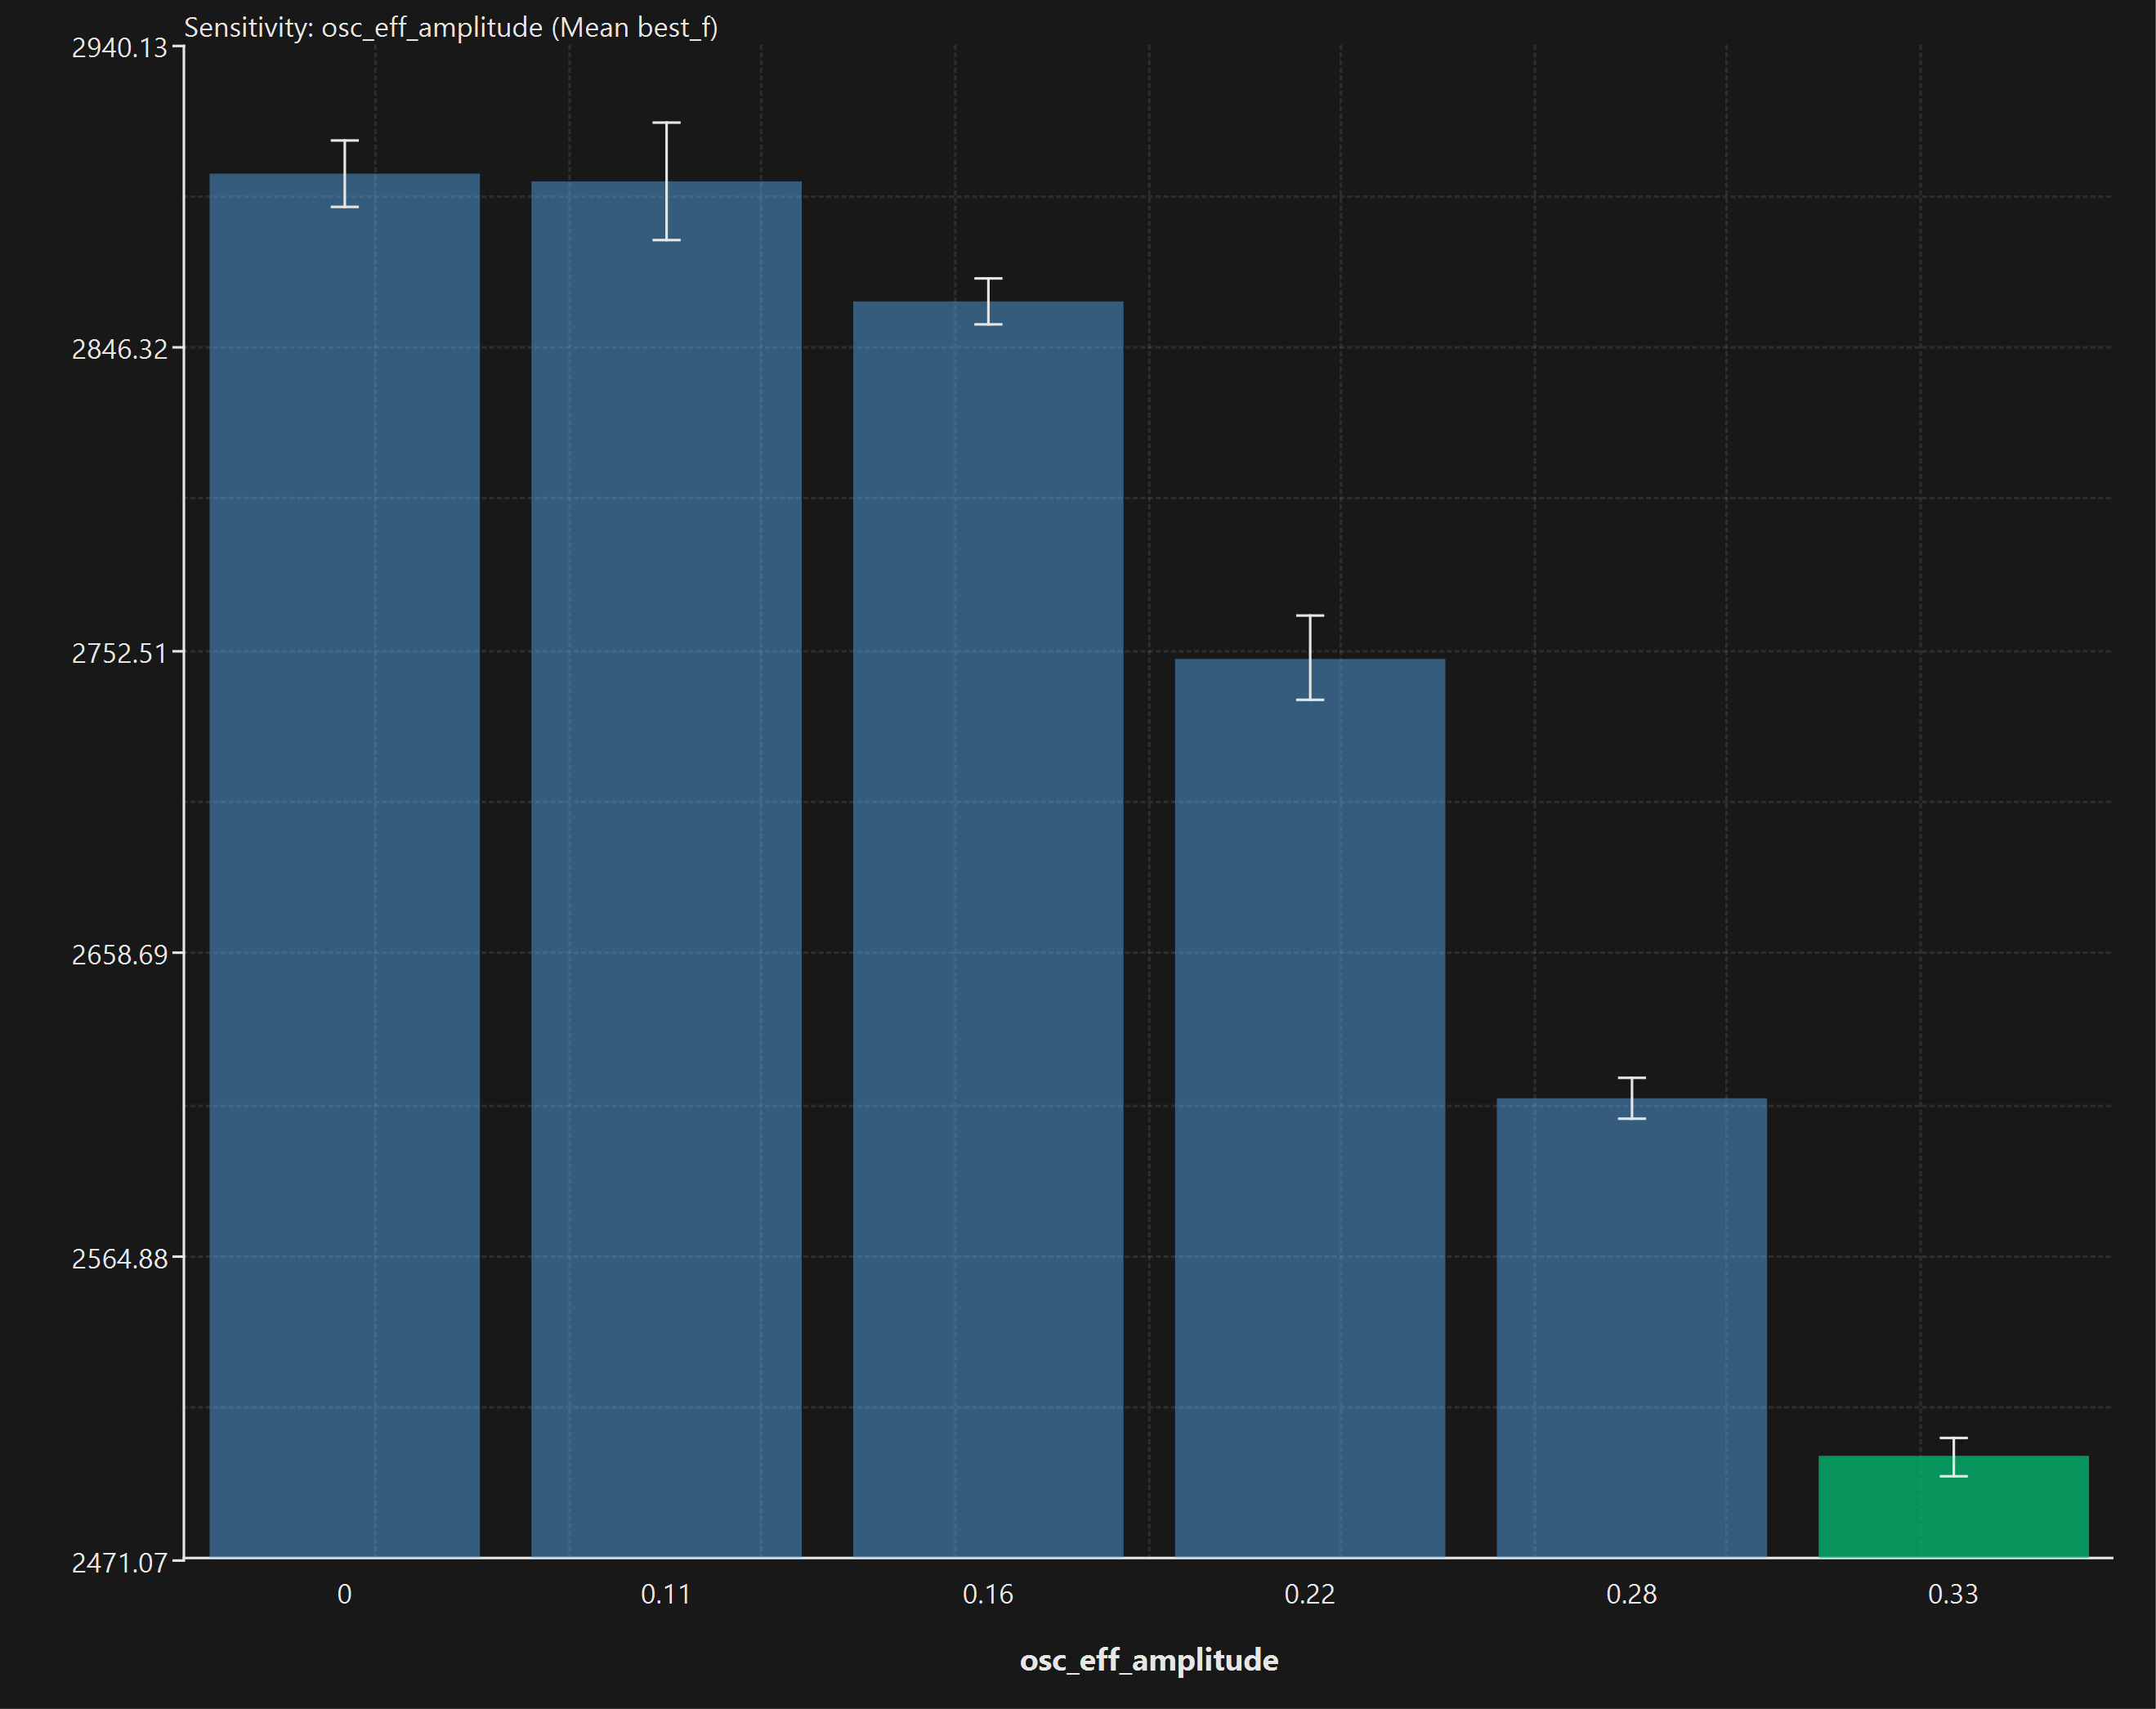
\includegraphics[scale=0.3]{mlshaderl_osc_eff_amplitude_weatherirrigation}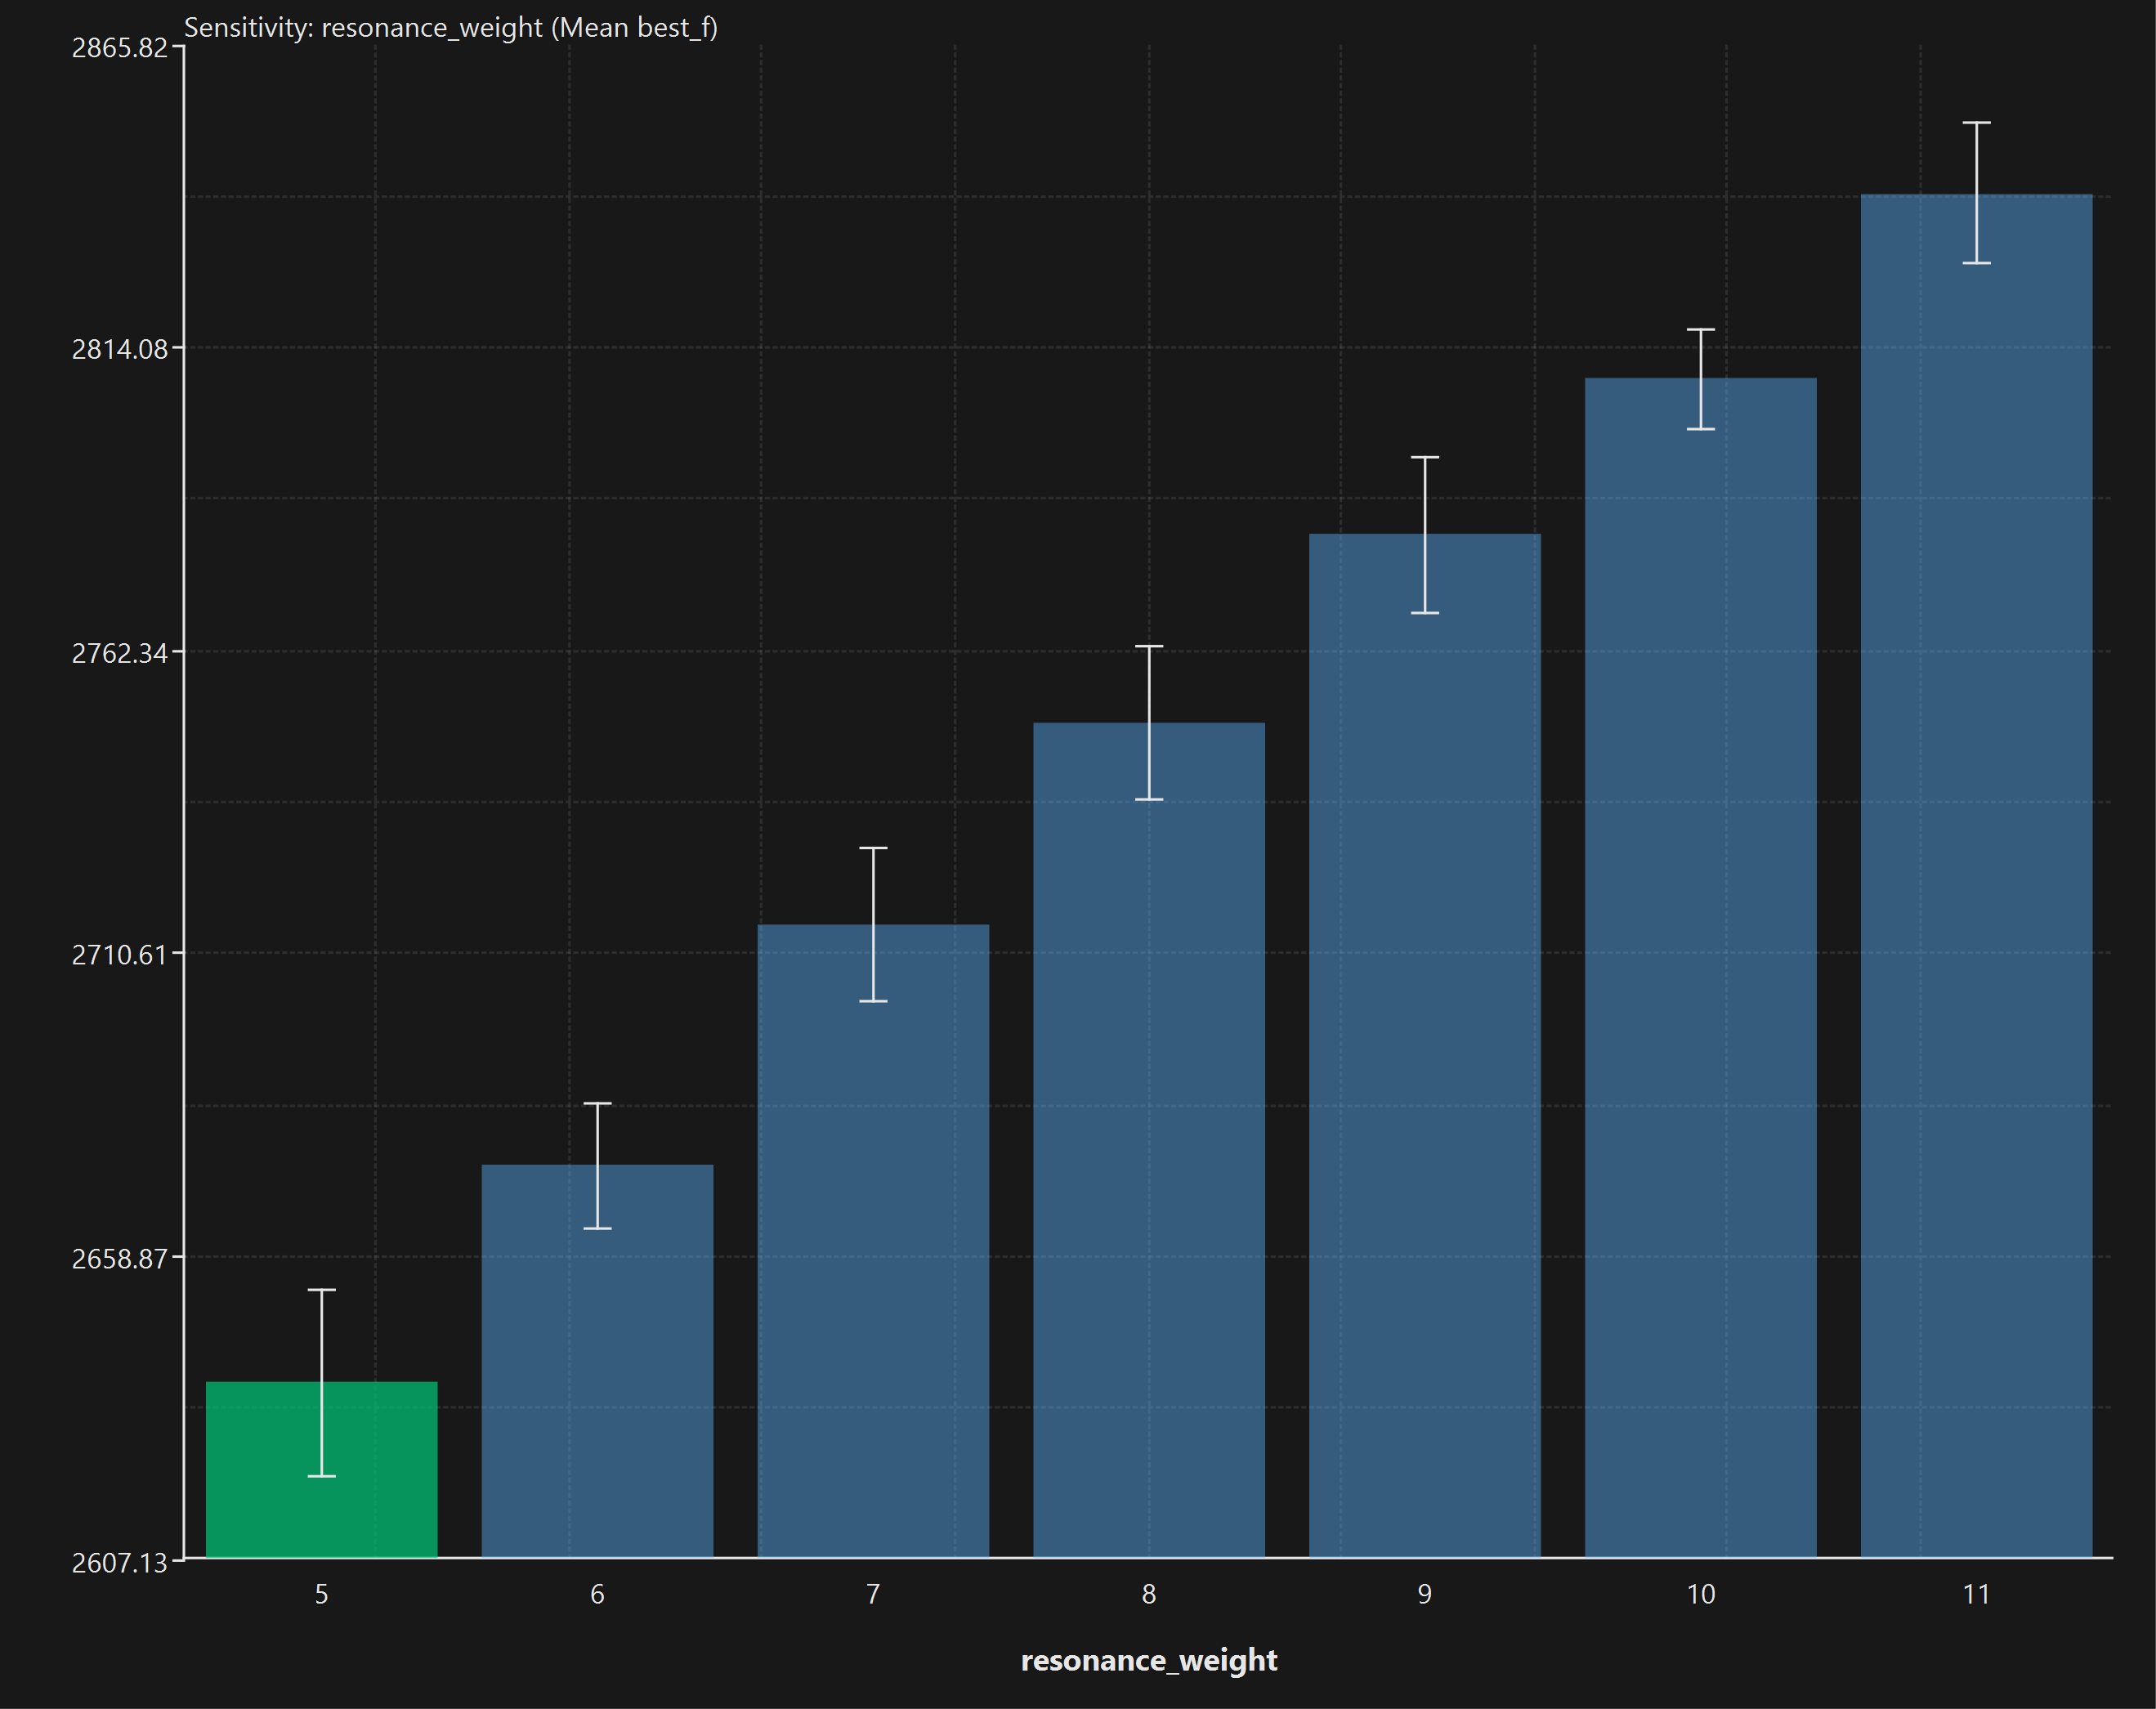
\includegraphics[scale=0.3]{mlshaderl_resonance_weight_weatherirrigation}
\par\end{centering}
\begin{centering}
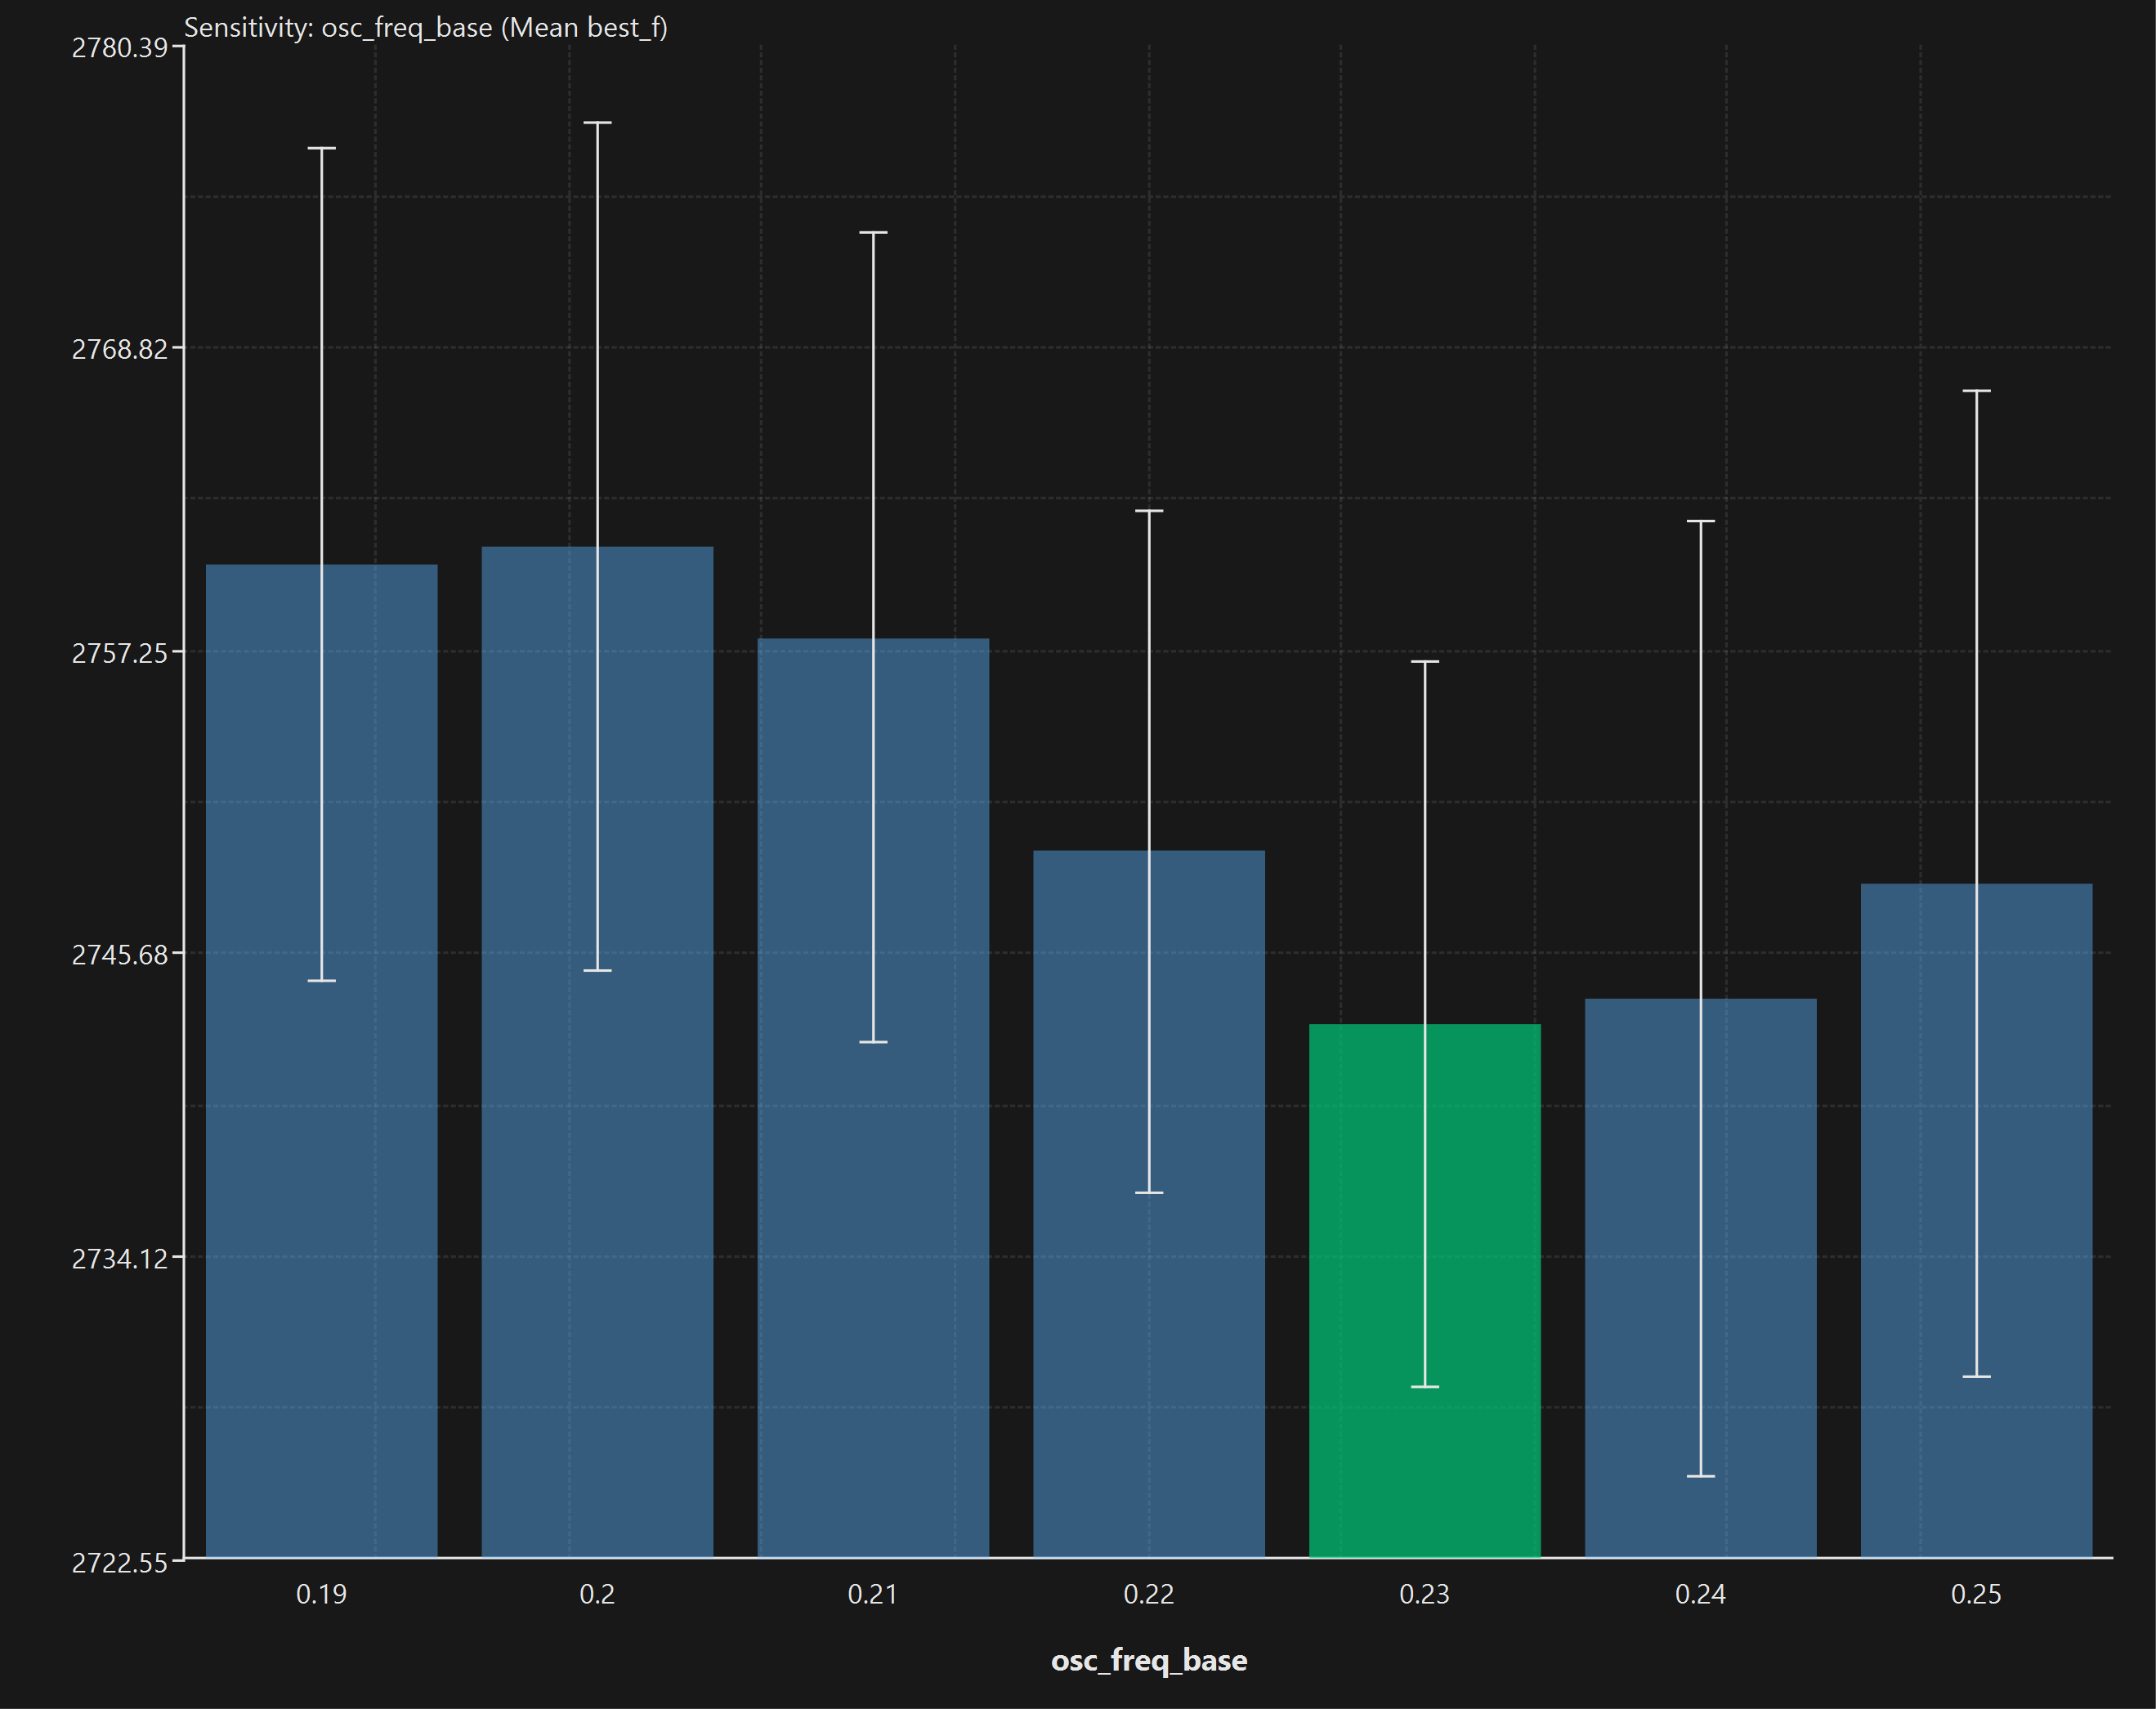
\includegraphics[scale=0.3]{mlshaderl_osc_freq_base_weatherirrigation}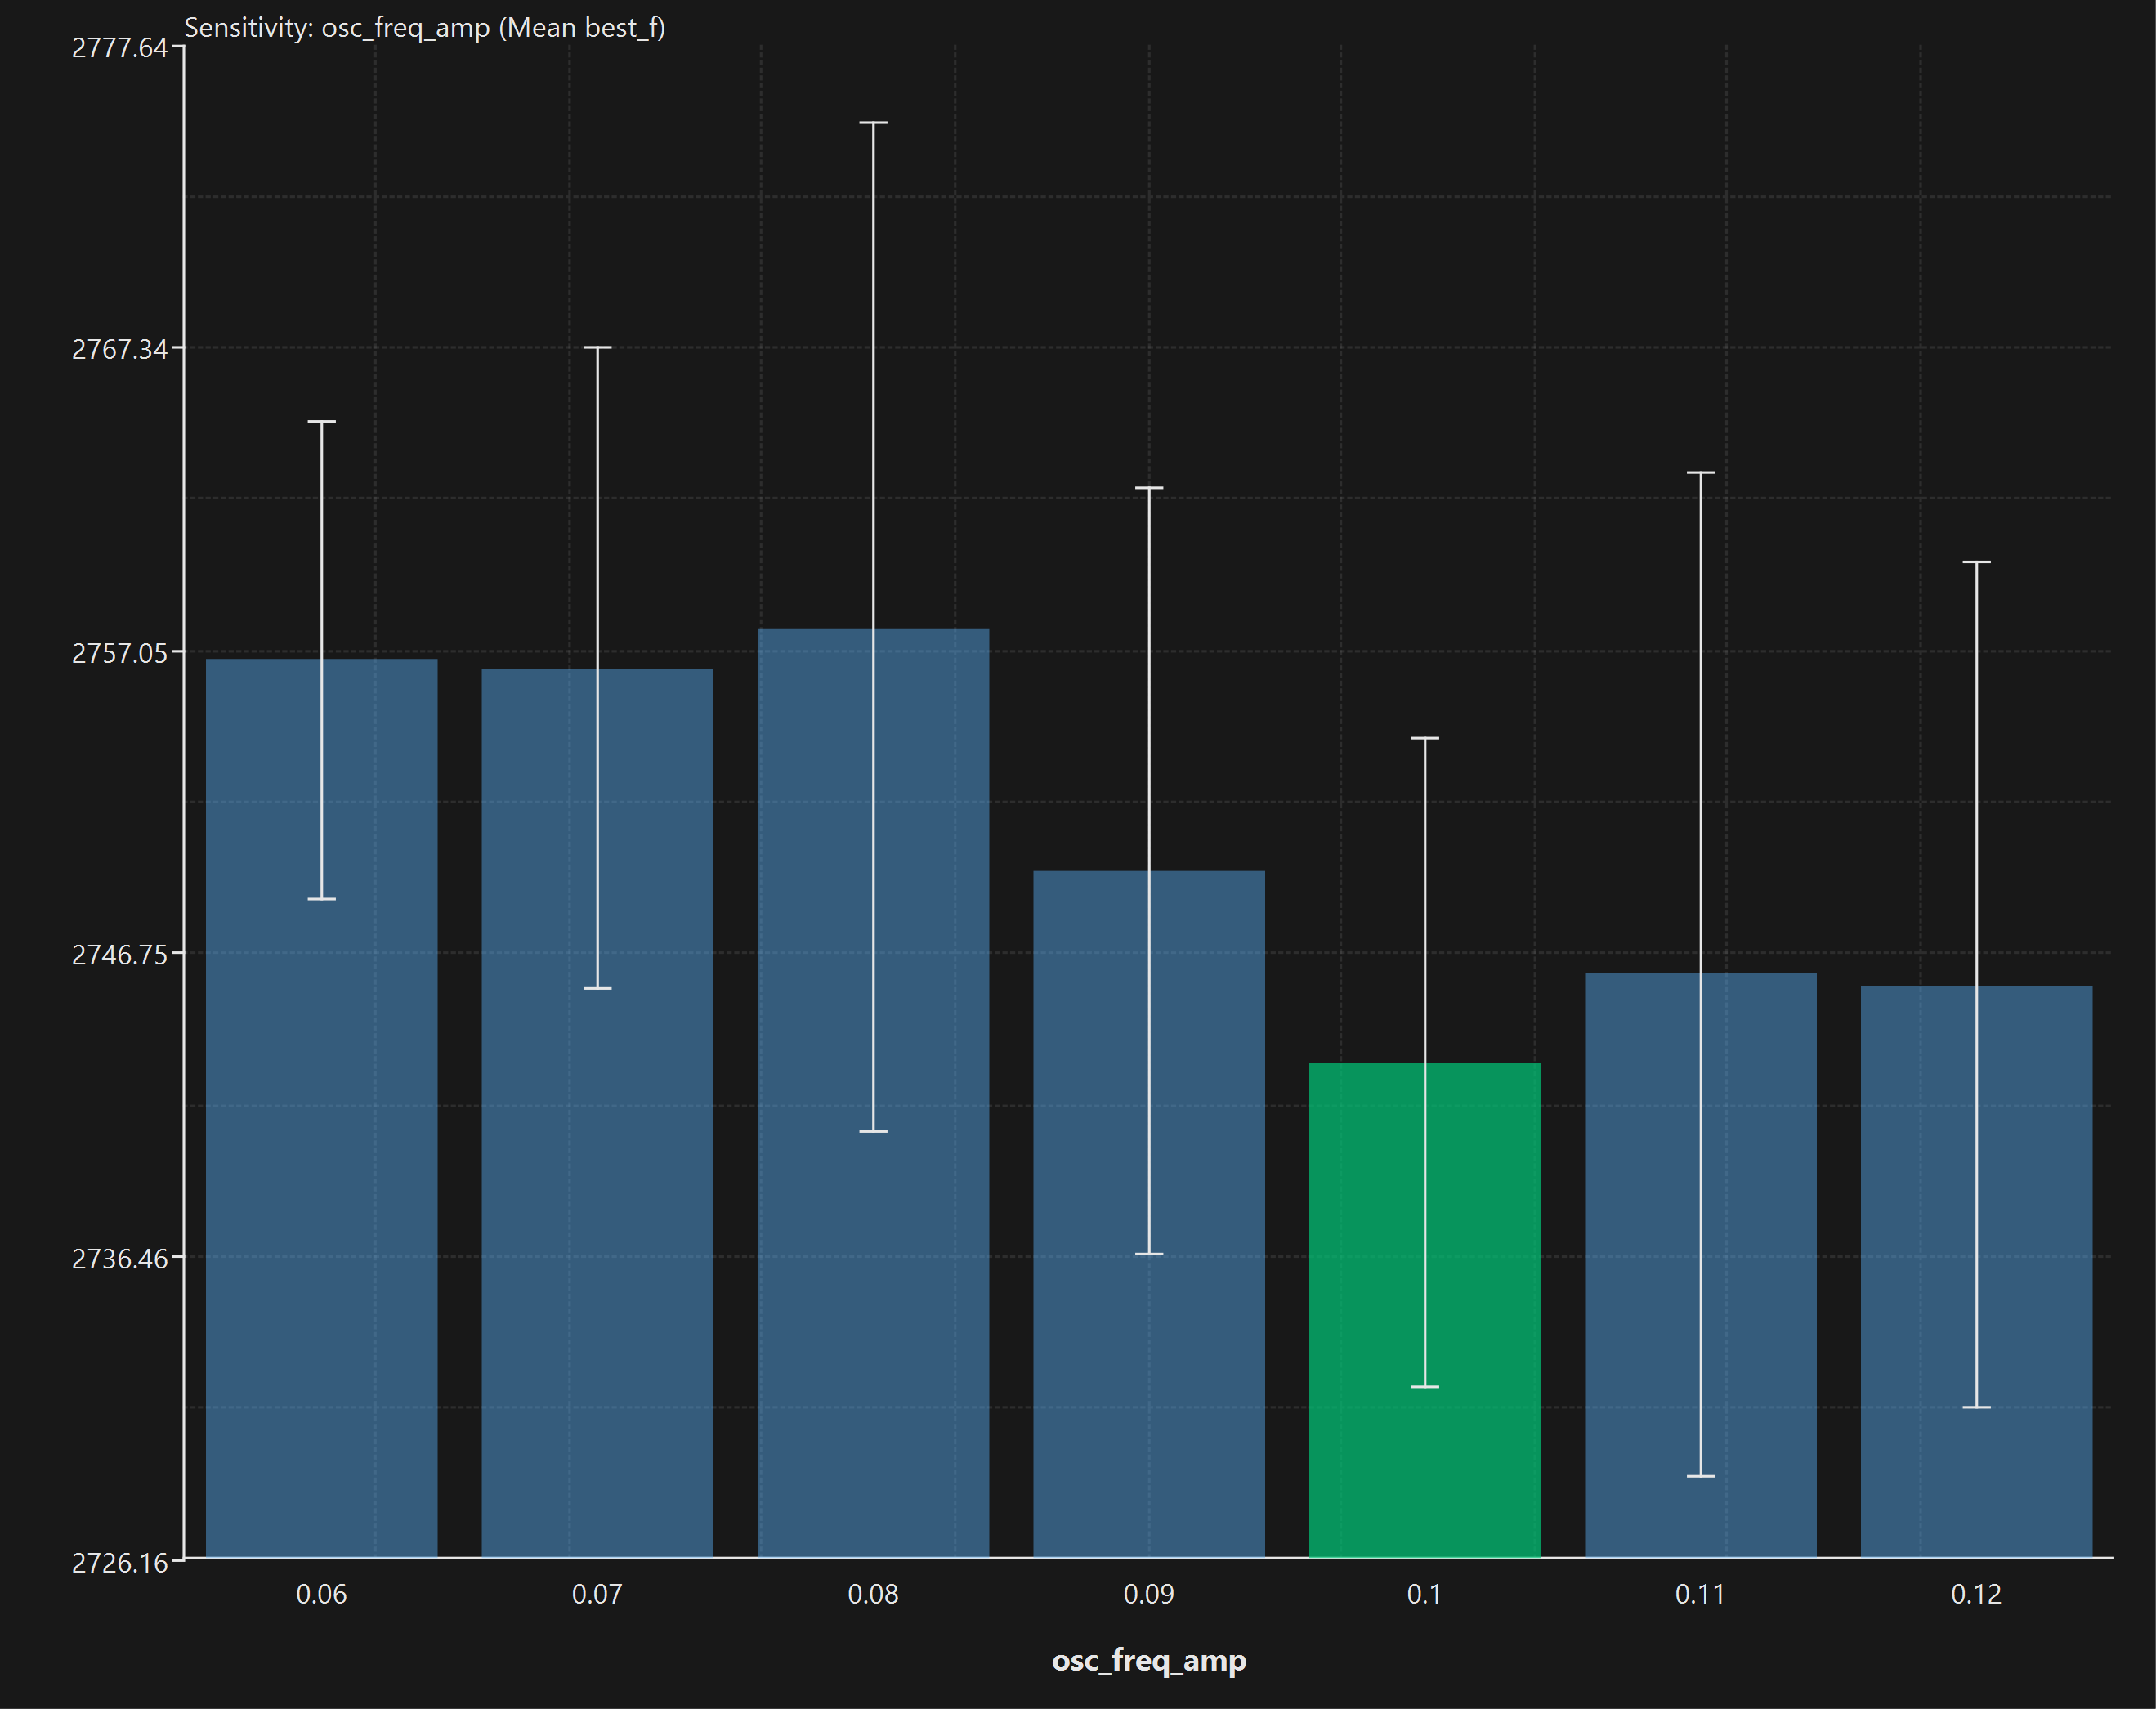
\includegraphics[scale=0.3]{mlshaderl_osc_freq_amp_weatherirrigation}
\par\end{centering}
\centering{}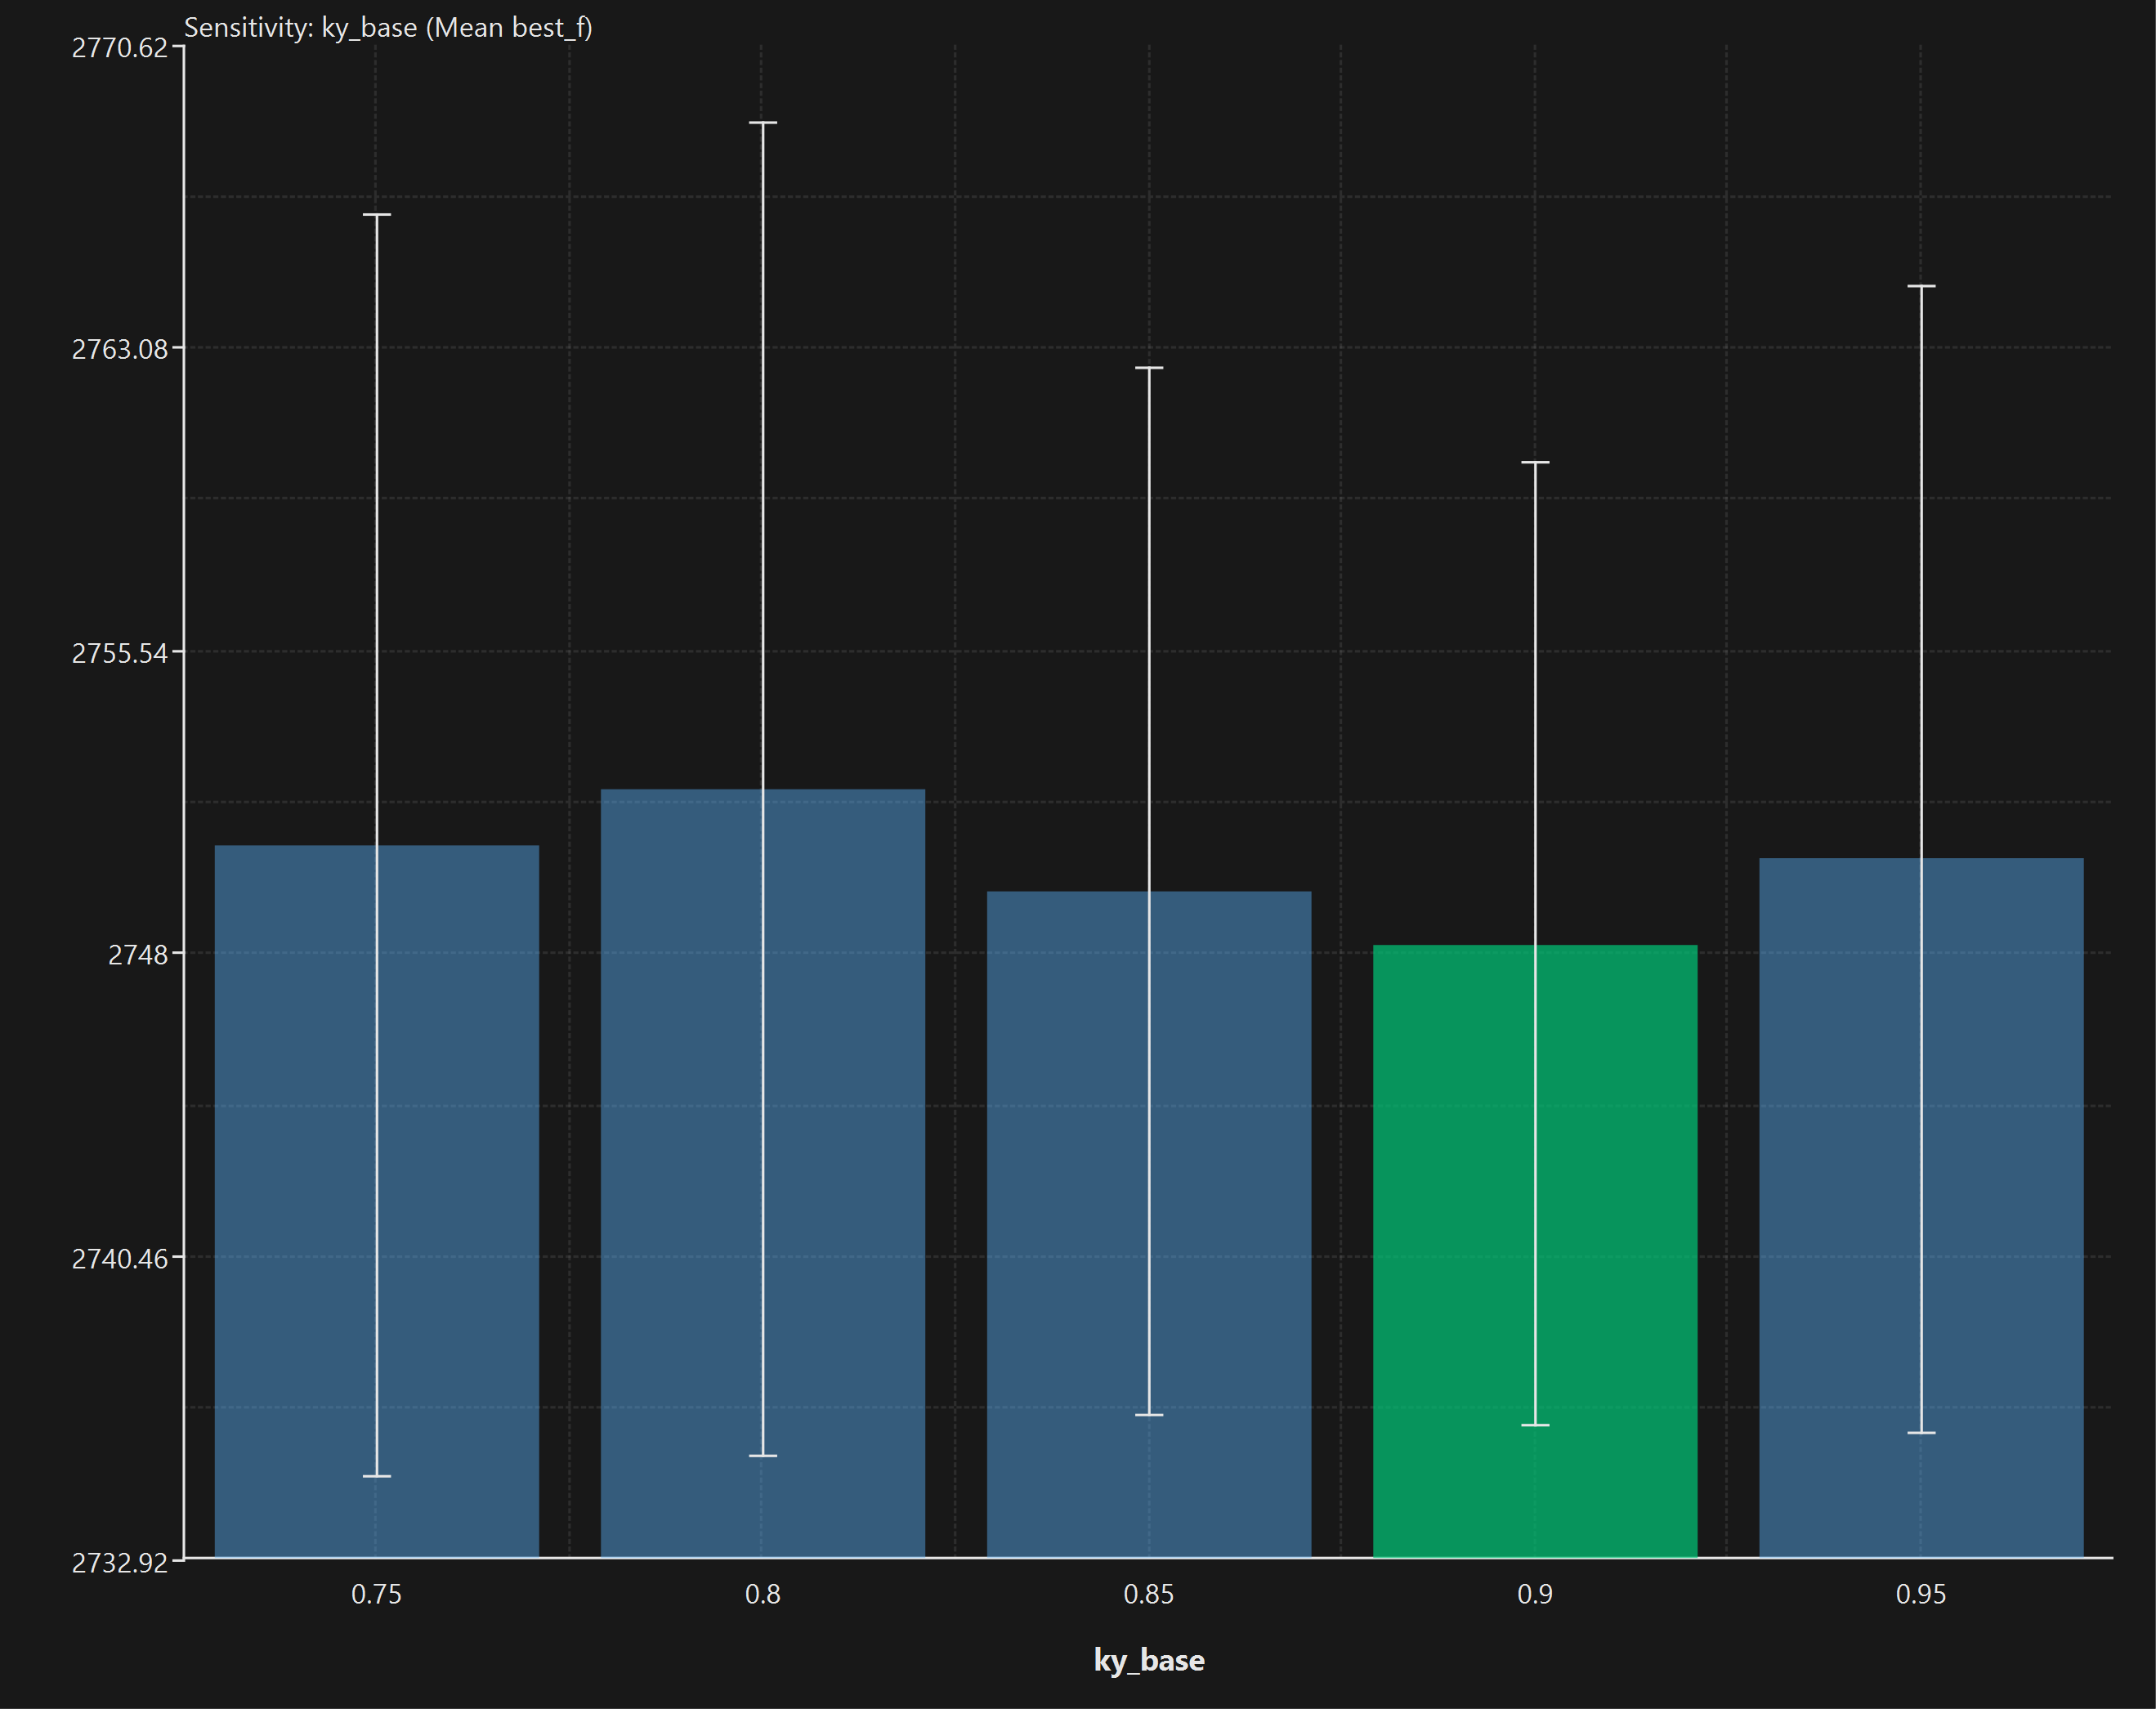
\includegraphics[scale=0.3]{mlshaderl_ky_base_weatherirrigation}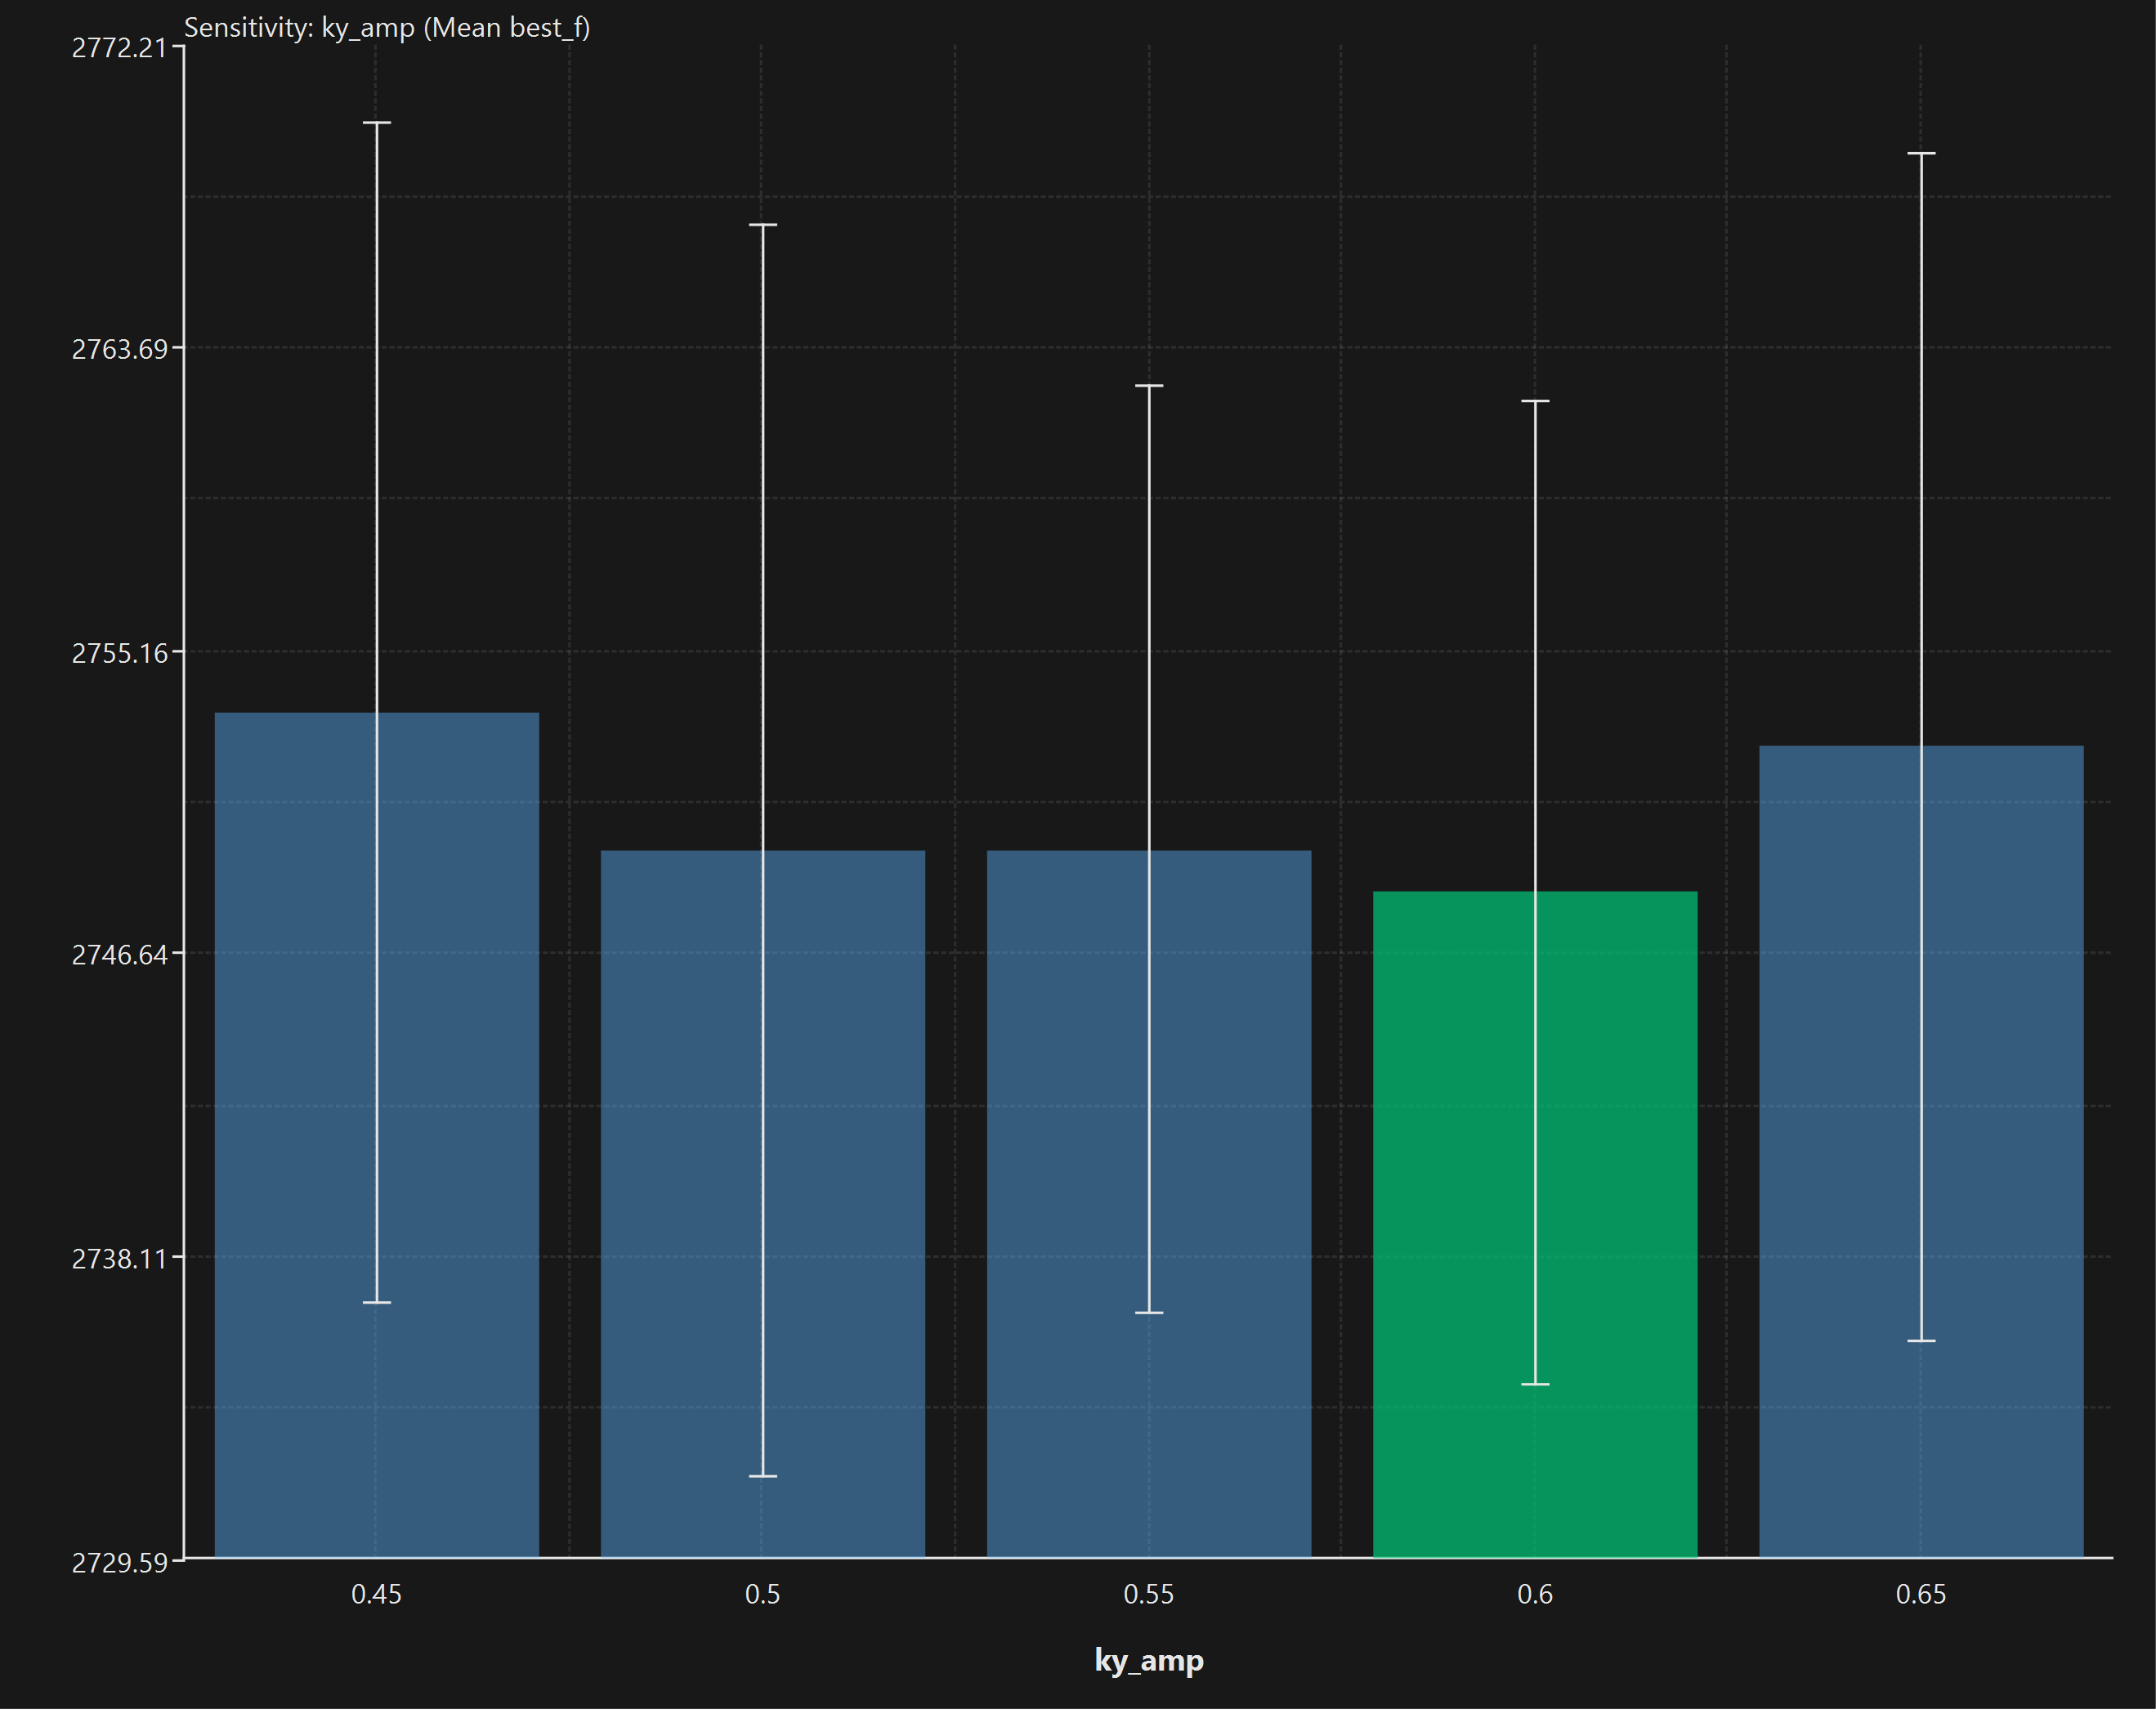
\includegraphics[scale=0.3]{mlshaderl_ky_amp_weatherirrigation}\caption{Mean best objective value as a function of each primary difficulty-controlling
parameter at $D=30$ (error bars denote $\pm1$ standard deviation
over 30 runs)\label{fig:sensitivity}}
\end{figure}

Figure \ref{fig:sensitivity} visualizes the sensitivity profiles
reported in Table \ref{tab:sensitivity}. The top-left panel confirms
the dominant and monotonically decreasing relationship between the
oscillatory efficiency amplitude and the mean best objective value.
The top-right panel shows the monotonically increasing effect of the
resonance weight. The middle panels reveal that the oscillation frequency
parameters produce only mild, non-monotonic variations within a narrow
band, suggesting that the density of local attractors is relatively
stable across the tested frequency range. The bottom panels confirm
the near-flat sensitivity to the yield-sensitivity coefficients, with
variations that fall within the inter-run standard deviation and are
therefore not statistically distinguishable from noise.

\subsection{Comparative Difficulty Assessment on Classical Benchmarks\label{subsec:otherProblems}}

To position the difficulty of the proposed benchmark relative to established
test functions, the seven optimizers that are common to both experiments
arq, clpso, cmaes, ga, jso, mlshaderl, and acor were evaluated on
four classical continuous optimization benchmarks at $D=30$ and $D=50$
under the same experimental protocol (30 independent runs, identical
evaluation budget). The four benchmark functions were selected to
represent distinct difficulty profiles that are individually present
in the proposed irrigation benchmark but rarely combined in a single
classical test function.

The Ackley function \citep{Ackley} is a widely used multimodal benchmark
with a nearly separable structure and an exponentially decaying envelope
that creates a broad basin surrounding the global optimum. It was
selected because its multimodal character provides a baseline for
assessing how the solvers handle oscillatory local structure in the
absence of inter-variable coupling. The Rastrigin function \citep{Rastrigin}
is a strongly multimodal, separable function whose cosine-based oscillatory
landscape produces a dense lattice of local minima a structure that
is directly analogous to the oscillatory efficiency modulation $\eta_{i}(x)$
embedded in the proposed benchmark. Its inclusion allows a controlled
comparison between separable and non-separable oscillatory difficulty.
The Rosenbrock function \citep{Rosenbrock} is a unimodal but non-separable
function characterized by a narrow curved valley, making it a standard
test for the ability of optimizers to follow non-separable gradient
structure. It was selected to isolate the contribution of non-separability
to search difficulty, independent of multimodality. The Schwefel function
\citep{Schwefel} features a deceptive global structure in which the
second-best local minimum is geometrically distant from the global
optimum, creating a landscape that misleads solvers toward suboptimal
regions. This deceptive character is analogous to the preferred-window
penalty $P_{win}$ and the multiplicative yield aggregation $Y_{rel}$
in the proposed benchmark. Table \ref{tab:otherProblems} reports
the complete results.

\begin{table}[H]
\caption{Comparative performance of seven optimizers on four classical benchmarks
and the proposed irrigation benchmark at $D=30$ and $D=50$ (30 independent
runs)\label{tab:otherProblems}}

\begin{centering}
\begin{tabular}{|c|c|c|c|c|c|c|c|c|}
\hline 
\multicolumn{9}{|c|}{{\footnotesize Ackley (multimodal, nearly separable)}}\tabularnewline
\hline 
\hline 
{\footnotesize Method} & \multicolumn{4}{c|}{{\footnotesize DIM = 30}} & \multicolumn{4}{c|}{{\footnotesize DIM = 50}}\tabularnewline
\hline 
 & {\footnotesize Value} & {\footnotesize Mean} & {\footnotesize Rate\%} & {\footnotesize SD} & {\footnotesize Value} & {\footnotesize Mean} & {\footnotesize Rate\%} & {\footnotesize SD}\tabularnewline
\hline 
{\footnotesize arq} & {\footnotesize 0.000} & {\footnotesize 0.000} & {\footnotesize 100} & {\footnotesize 0.000} & {\footnotesize 0.000} & {\footnotesize 0.866} & {\footnotesize 37} & {\footnotesize 0.698}\tabularnewline
\hline 
{\footnotesize clpso} & {\footnotesize 1.849} & {\footnotesize 2.238} & {\footnotesize 3} & {\footnotesize 0.160} & {\footnotesize 4.466} & {\footnotesize 4.887} & {\footnotesize 3} & {\footnotesize 0.230}\tabularnewline
\hline 
{\footnotesize cmaes} & {\footnotesize 0.000} & {\footnotesize 0.000} & {\footnotesize 100} & {\footnotesize 0.000} & {\footnotesize 0.000} & {\footnotesize 0.000} & {\footnotesize 100} & {\footnotesize 0.000}\tabularnewline
\hline 
{\footnotesize ga} & {\footnotesize 1.809} & {\footnotesize 5.312} & {\footnotesize 3} & {\footnotesize 2.887} & {\footnotesize 6.105} & {\footnotesize 11.290} & {\footnotesize 3} & {\footnotesize 3.083}\tabularnewline
\hline 
{\footnotesize jso} & {\footnotesize 0.000} & {\footnotesize 0.000} & {\footnotesize 100} & {\footnotesize 0.000} & {\footnotesize 0.000} & {\footnotesize 0.000} & {\footnotesize 100} & {\footnotesize 0.000}\tabularnewline
\hline 
{\footnotesize mlshaderl} & {\footnotesize 0.000} & {\footnotesize 0.000} & {\footnotesize 100} & {\footnotesize 0.000} & {\footnotesize 0.000} & {\footnotesize 0.000} & {\footnotesize 100} & {\footnotesize 0.000}\tabularnewline
\hline 
{\footnotesize acor} & {\footnotesize 0.000} & {\footnotesize 0.000} & {\footnotesize 100} & {\footnotesize 0.000} & {\footnotesize 0.001} & {\footnotesize 0.002} & {\footnotesize 3} & {\footnotesize 0.000}\tabularnewline
\hline 
\multicolumn{9}{|c|}{{\footnotesize Rastrigin (multimodal, separable)}}\tabularnewline
\hline 
{\footnotesize Method} & \multicolumn{4}{c|}{{\footnotesize DIM = 30}} & \multicolumn{4}{c|}{{\footnotesize DIM = 50}}\tabularnewline
\hline 
 & {\footnotesize Value} & {\footnotesize Mean} & {\footnotesize Rate\%} & {\footnotesize SD} & {\footnotesize Value} & {\footnotesize Mean} & {\footnotesize Rate\%} & {\footnotesize SD}\tabularnewline
\hline 
{\footnotesize arq} & {\footnotesize 0.000} & {\footnotesize 0.431} & {\footnotesize 70} & {\footnotesize 0.770} & {\footnotesize 0.000} & {\footnotesize 2.753} & {\footnotesize 10} & {\footnotesize 1.766}\tabularnewline
\hline 
{\footnotesize clpso} & {\footnotesize 45.562} & {\footnotesize 55.445} & {\footnotesize 3} & {\footnotesize 5.967} & {\footnotesize 163.202} & {\footnotesize 179.140} & {\footnotesize 3} & {\footnotesize 8.682}\tabularnewline
\hline 
{\footnotesize cmaes} & {\footnotesize 0.000} & {\footnotesize 0.000} & {\footnotesize 100} & {\footnotesize 0.000} & {\footnotesize 0.000} & {\footnotesize 0.000} & {\footnotesize 100} & {\footnotesize 0.000}\tabularnewline
\hline 
{\footnotesize ga} & {\footnotesize 34.603} & {\footnotesize 75.510} & {\footnotesize 3} & {\footnotesize 20.113} & {\footnotesize 125.429} & {\footnotesize 211.418} & {\footnotesize 3} & {\footnotesize 32.690}\tabularnewline
\hline 
{\footnotesize jso} & {\footnotesize 0.000} & {\footnotesize 0.199} & {\footnotesize 97} & {\footnotesize 1.090} & {\footnotesize 0.000} & {\footnotesize 0.033} & {\footnotesize 3} & {\footnotesize 0.182}\tabularnewline
\hline 
{\footnotesize mlshaderl} & {\footnotesize 0.000} & {\footnotesize 3.051} & {\footnotesize 3} & {\footnotesize 1.751} & {\footnotesize 5.970} & {\footnotesize 11.475} & {\footnotesize 3} & {\footnotesize 2.965}\tabularnewline
\hline 
{\footnotesize acor} & {\footnotesize 173.137} & {\footnotesize 199.811} & {\footnotesize 3} & {\footnotesize 12.340} & {\footnotesize 355.488} & {\footnotesize 436.769} & {\footnotesize 3} & {\footnotesize 21.310}\tabularnewline
\hline 
\multicolumn{9}{|c|}{{\footnotesize Rosenbrock (unimodal, non-separable)}}\tabularnewline
\hline 
{\footnotesize Method} & \multicolumn{4}{c|}{{\footnotesize DIM = 30}} & \multicolumn{4}{c|}{{\footnotesize DIM = 50}}\tabularnewline
\hline 
 & {\footnotesize Value} & {\footnotesize Mean} & {\footnotesize Rate\%} & {\footnotesize SD} & {\footnotesize Value} & {\footnotesize Mean} & {\footnotesize Rate\%} & {\footnotesize SD}\tabularnewline
\hline 
{\footnotesize arq} & {\footnotesize 0.000} & {\footnotesize 0.000} & {\footnotesize 100} & {\footnotesize 0.000} & {\footnotesize 0.068} & {\footnotesize 2.237} & {\footnotesize 3} & {\footnotesize 2.012}\tabularnewline
\hline 
{\footnotesize clpso} & {\footnotesize 43.541} & {\footnotesize 66.203} & {\footnotesize 3} & {\footnotesize 12.374} & {\footnotesize 137.479} & {\footnotesize 182.123} & {\footnotesize 3} & {\footnotesize 19.021}\tabularnewline
\hline 
{\footnotesize cmaes} & {\footnotesize 0.000} & {\footnotesize 0.532} & {\footnotesize 87} & {\footnotesize 1.378} & {\footnotesize 0.000} & {\footnotesize 0.266} & {\footnotesize 93} & {\footnotesize 1.011}\tabularnewline
\hline 
{\footnotesize ga} & {\footnotesize 1.403} & {\footnotesize 9.352} & {\footnotesize 3} & {\footnotesize 13.548} & {\footnotesize 40.653} & {\footnotesize 121.036} & {\footnotesize 3} & {\footnotesize 46.509}\tabularnewline
\hline 
{\footnotesize jso} & {\footnotesize 0.000} & {\footnotesize 0.000} & {\footnotesize 100} & {\footnotesize 0.000} & {\footnotesize 0.055} & {\footnotesize 2.460} & {\footnotesize 3} & {\footnotesize 2.045}\tabularnewline
\hline 
{\footnotesize mlshaderl} & {\footnotesize 0.000} & {\footnotesize 0.000} & {\footnotesize 90} & {\footnotesize 0.000} & {\footnotesize 3.677} & {\footnotesize 8.275} & {\footnotesize 3} & {\footnotesize 2.603}\tabularnewline
\hline 
{\footnotesize acor} & {\footnotesize 22.949} & {\footnotesize 23.486} & {\footnotesize 3} & {\footnotesize 0.169} & {\footnotesize 44.703} & {\footnotesize 46.257} & {\footnotesize 3} & {\footnotesize 0.366}\tabularnewline
\hline 
\multicolumn{9}{|c|}{{\footnotesize Schwefel (deceptive global structure)}}\tabularnewline
\hline 
{\footnotesize Method} & \multicolumn{4}{c|}{{\footnotesize DIM = 30}} & \multicolumn{4}{c|}{{\footnotesize DIM = 50}}\tabularnewline
\hline 
 & {\footnotesize Value} & {\footnotesize Mean} & {\footnotesize Rate\%} & {\footnotesize SD} & {\footnotesize Value} & {\footnotesize Mean} & {\footnotesize Rate\%} & {\footnotesize SD}\tabularnewline
\hline 
{\footnotesize arq} & {\footnotesize 236.877} & {\footnotesize 911.163} & {\footnotesize 3} & {\footnotesize 422.393} & {\footnotesize 2260.948} & {\footnotesize 3257.192} & {\footnotesize 7} & {\footnotesize 554.197}\tabularnewline
\hline 
{\footnotesize clpso} & {\footnotesize 135.272} & {\footnotesize 472.769} & {\footnotesize 3} & {\footnotesize 140.728} & {\footnotesize 2993.371} & {\footnotesize 4204.992} & {\footnotesize 3} & {\footnotesize 457.860}\tabularnewline
\hline 
{\footnotesize cmaes} & {\footnotesize 3217.735} & {\footnotesize 4922.821} & {\footnotesize 3} & {\footnotesize 649.304} & {\footnotesize 6300.446} & {\footnotesize 8278.018} & {\footnotesize 3} & {\footnotesize 937.601}\tabularnewline
\hline 
{\footnotesize ga} & {\footnotesize 0.082} & {\footnotesize 25.188} & {\footnotesize 3} & {\footnotesize 48.552} & {\footnotesize 126.888} & {\footnotesize 347.795} & {\footnotesize 3} & {\footnotesize 154.861}\tabularnewline
\hline 
{\footnotesize jso} & {\footnotesize 0.000} & {\footnotesize 467.833} & {\footnotesize 7} & {\footnotesize 331.048} & {\footnotesize 1618.663} & {\footnotesize 3342.078} & {\footnotesize 3} & {\footnotesize 1600.885}\tabularnewline
\hline 
{\footnotesize mlshaderl} & {\footnotesize 0.000} & {\footnotesize 86.906} & {\footnotesize 40} & {\footnotesize 102.922} & {\footnotesize 118.439} & {\footnotesize 609.521} & {\footnotesize 10} & {\footnotesize 398.185}\tabularnewline
\hline 
{\footnotesize acor} & {\footnotesize 7541.236} & {\footnotesize 7958.509} & {\footnotesize 3} & {\footnotesize 183.466} & {\footnotesize 14020.958} & {\footnotesize 14871.290} & {\footnotesize 3} & {\footnotesize 329.079}\tabularnewline
\hline 
\multicolumn{9}{|c|}{{\footnotesize Proposed benchmark (full formulation, $ALL$)}}\tabularnewline
\hline 
{\footnotesize Method} & \multicolumn{4}{c|}{{\footnotesize DIM = 30}} & \multicolumn{4}{c|}{{\footnotesize DIM = 50}}\tabularnewline
\hline 
 & {\footnotesize Value} & {\footnotesize Mean} & {\footnotesize Rate\%} & {\footnotesize SD} & {\footnotesize Value} & {\footnotesize Mean} & {\footnotesize Rate\%} & {\footnotesize SD}\tabularnewline
\hline 
{\footnotesize arq} & {\footnotesize 2736.355} & {\footnotesize 2769.033} & {\footnotesize 3} & {\footnotesize 19.880} & {\footnotesize 6802.897} & {\footnotesize 6836.089} & {\footnotesize 3} & {\footnotesize 21.400}\tabularnewline
\hline 
{\footnotesize clpso} & {\footnotesize 2744.664} & {\footnotesize 2750.093} & {\footnotesize 3} & {\footnotesize 3.803} & {\footnotesize 6861.143} & {\footnotesize 6874.249} & {\footnotesize 3} & {\footnotesize 8.224}\tabularnewline
\hline 
{\footnotesize cmaes} & {\footnotesize 2739.460} & {\footnotesize 2778.598} & {\footnotesize 3} & {\footnotesize 26.858} & {\footnotesize 6801.328} & {\footnotesize 6830.234} & {\footnotesize 3} & {\footnotesize 15.765}\tabularnewline
\hline 
{\footnotesize ga} & {\footnotesize 2764.424} & {\footnotesize 2837.572} & {\footnotesize 3} & {\footnotesize 47.075} & {\footnotesize 6940.318} & {\footnotesize 7265.921} & {\footnotesize 3} & {\footnotesize 212.781}\tabularnewline
\hline 
{\footnotesize jso} & {\footnotesize 2737.798} & {\footnotesize 2744.379} & {\footnotesize 3} & {\footnotesize 5.791} & {\footnotesize 6788.850} & {\footnotesize 6806.872} & {\footnotesize 3} & {\footnotesize 9.409}\tabularnewline
\hline 
{\footnotesize mlshaderl} & {\footnotesize 2736.355} & {\footnotesize 2749.478} & {\footnotesize 10} & {\footnotesize 13.045} & {\footnotesize 6787.179} & {\footnotesize 6815.552} & {\footnotesize 3} & {\footnotesize 18.727}\tabularnewline
\hline 
{\footnotesize acor} & {\footnotesize 2737.798} & {\footnotesize 2772.389} & {\footnotesize 3} & {\footnotesize 15.015} & {\footnotesize 6784.162} & {\footnotesize 6785.259} & {\footnotesize 3} & {\footnotesize 1.446}\tabularnewline
\hline 
\end{tabular}
\par\end{centering}
\end{table}

The results in Table \ref{tab:otherProblems} reveal a striking contrast
between the difficulty of the classical benchmarks and that of the
proposed irrigation benchmark. On Ackley at $D=50$, five out of seven
solvers (arq, cmaes, jso, mlshaderl, and acor at $D=30$) achieve
success rates of 100\%, and cmaes, jso, and mlshaderl maintain 100\%
at $D=50$. This confirms that multimodality alone, when combined
with near-separability and a smooth global envelope, is readily handled
by modern continuous optimizers. The Rastrigin function, which presents
a denser lattice of local minima, is more challenging: at $D=50$,
only cmaes achieves 100\%, while arq drops to 10\% and most other
methods fall to 3\%. Nevertheless, the best-performing solvers maintain
high reliability, indicating that separable oscillatory structure,
even when dense, does not constitute a fundamental barrier for methods
with adequate covariance adaptation or restart mechanisms.

The Rosenbrock function introduces non-separability without multimodality.
At $D=30$, arq and jso both achieve 100\%, and cmaes 87\%. At $D=50$,
cmaes maintains a success rate of 93\%, demonstrating that non-separable
valley structure alone remains tractable for covariance-based methods.
The Schwefel function presents the closest difficulty profile to the
proposed benchmark among the four classical functions: at $D=30$,
only mlshaderl achieves a meaningful success rate (40\%), and at $D=50$,
mlshaderl drops to 10\% and all other methods to 7\% or below. The
deceptive global structure of Schwefel thus represents a genuine challenge,
but one that is still partially navigable by archive-based methods.

By comparison, the proposed irrigation benchmark at $D=30$ yields
a maximum success rate of only 10\% (mlshaderl), and at $D=50$, all
seven methods achieve the minimum rate of 3\% without exception. This
represents a qualitative step beyond even the Schwefel function in
terms of search difficulty. The explanation lies in the simultaneous
presence of mechanisms that the classical functions present only in
isolation: the proposed benchmark combines the dense oscillatory local
structure of Rastrigin (through $\eta_{i}(x)$), the non-separable
coupling of Rosenbrock (through the recursive storage $S_{i}$ and
the neighbor load $N_{i}$), the deceptive global structure of Schwefel
(through $P_{win}$ and the multiplicative $Y_{rel})$, and a stateful
path dependence that is entirely absent from all four classical functions.
This combination creates a landscape in which no single algorithmic
capability whether covariance adaptation, archive-based memory, or
probability density estimation is sufficient to ensure reliable convergence,
confirming that the proposed benchmark occupies a difficulty regime
that is not adequately represented by existing classical test functions.

\subsection{Statistical Validation\label{subsec:stats}}

To confirm that the performance differences observed in Section 2.4
are statistically significant rather than artifacts of run-to-run
variability, a nonparametric statistical analysis was conducted on
the 30 final objective values obtained by each method on the full
benchmark formulation ($ALL$) across all five dimensions. The Friedman
test was applied independently at each dimension to assess whether
the eight methods produce significantly different rank distributions.
Pairwise comparisons were then performed using Wilcoxon signed-rank
tests with Holm correction to control the family-wise error rate.
Table \ref{tab:friedman} reports the mean Friedman ranks for each
method at each dimension, together with the overall average rank and
the Friedman test p-values.

\begin{table}[H]
\caption{Mean Friedman ranks of the eight optimizers on the full benchmark
formulation across all dimensions (30 independent runs, lower rank
indicates better performance)\label{tab:friedman}}

\begin{centering}
\begin{tabular}{|c|c|c|c|c|c|c|}
\hline 
Method & D=24 & D=30 & D=50 & D=70 & D=100 & Avg\tabularnewline
\hline 
\hline 
jso & 1.87 & 1.88 & 2.47 & 2.57 & 2 & 2.16\tabularnewline
\hline 
mlshaderl & 2.77 & 2.6 & 3.13 & 2.33 & 2.37 & 2.64\tabularnewline
\hline 
acor & 2.57 & 4.6 & 1 & 3.07 & 6.07 & 3.46\tabularnewline
\hline 
cmaes & 4.5 & 4.7 & 4.17 & 2.5 & 1.63 & 3.5\tabularnewline
\hline 
arq & 3.67 & 4.55 & 4.33 & 4.57 & 4.03 & 4.23\tabularnewline
\hline 
clpso & 5.8 & 2.97 & 5.9 & 5.97 & 4.97 & 5.12\tabularnewline
\hline 
ga & 7.23 & 6.97 & 7.2 & 7.07 & 6.97 & 7.09\tabularnewline
\hline 
gwo & 7.6 & 7.73 & 7.8 & 7.93 & 7.97 & 7.81\tabularnewline
\hline 
Friedman p & 2.01e-32 & 1.55e-28 & 4.12e-38 & 2.12e-34 & 1.12e-39 & \tabularnewline
\hline 
\end{tabular}
\par\end{centering}
\end{table}

The Friedman test rejects the null hypothesis of equal method performance
at all five dimensions with p-values below $10^{-28}$, confirming
that the observed differences are highly significant. The mean ranks
identify jso as the best-performing method overall (average rank 2.16),
followed by mlshaderl (2.64), acor (3.46), and cmaes (3.50). The methods
ga (7.09) and gwo (7.81) consistently occupy the lowest ranks, confirming
their poor suitability for this benchmark. Notably, the ranking of
acor shifts substantially across dimensions: it achieves the best
rank at D = 50 (1.00) but deteriorates to 6.07 at $D=100$, suggesting
that its probability density estimation mechanism is highly effective
at moderate dimensions but loses precision as the search space grows.
Pairwise Wilcoxon tests with Holm correction confirm that jso and
mlshaderl differ significantly from ga and gwo at all dimensions (p
\textless{} 0.001), while the differences among the top four methods
(jso, mlshaderl, acor, cmaes) are significant at most but not all
dimensions, reflecting the competitive and complementary nature of
their search strategies. Figure \ref{fig:friedman} visualizes the
rank structure across dimensions, and Figure \ref{fig:distribution}
shows the corresponding distributions of final objective values.

\begin{figure}[H]
\begin{centering}
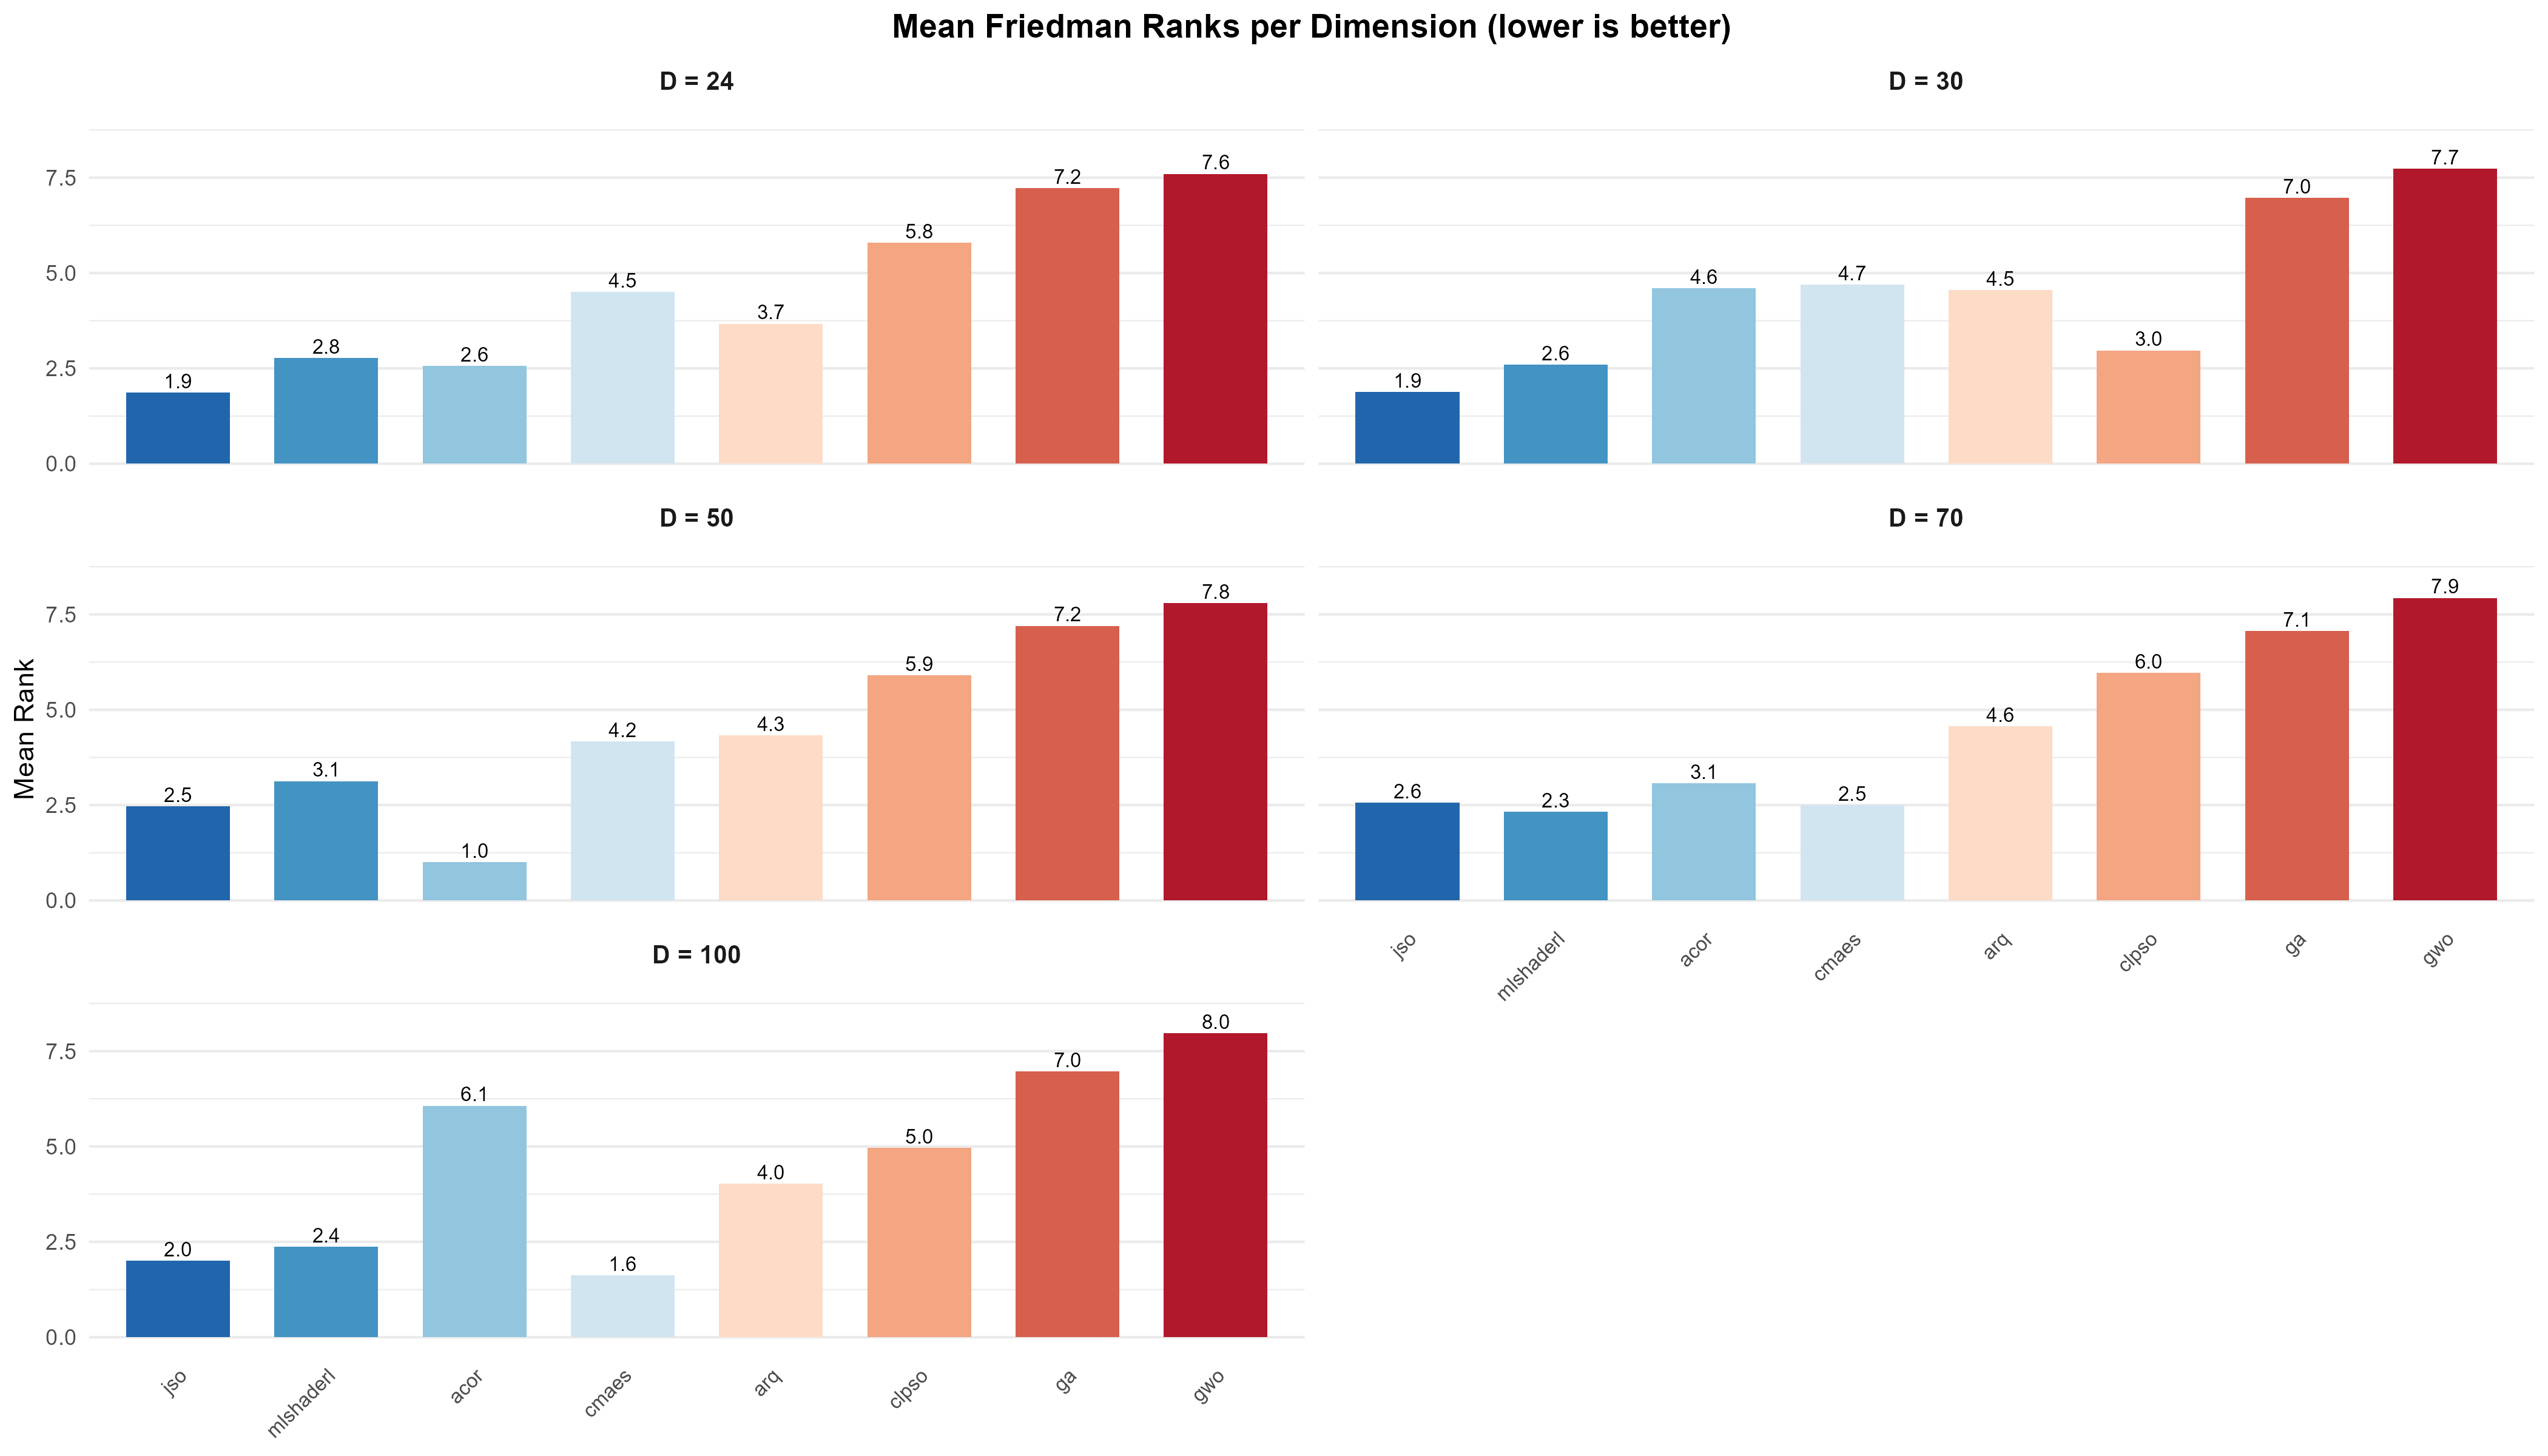
\includegraphics[scale=0.4]{mean_ranks}
\par\end{centering}
\caption{Mean Friedman ranks per dimension for the full benchmark formulation
(lower is better)\label{fig:friedman}}

\end{figure}

Figure \ref{fig:friedman} confirms visually that jso and mlshaderl
maintain consistently low ranks across all dimensions, while ga and
gwo are stably positioned at ranks 7-8. The intermediate methods (acor,
cmaes, arq, clpso) exhibit dimension-dependent rank shifts that reflect
the varying effectiveness of their search mechanisms as the landscape
complexity scales with D.

\begin{figure}[H]
\begin{centering}
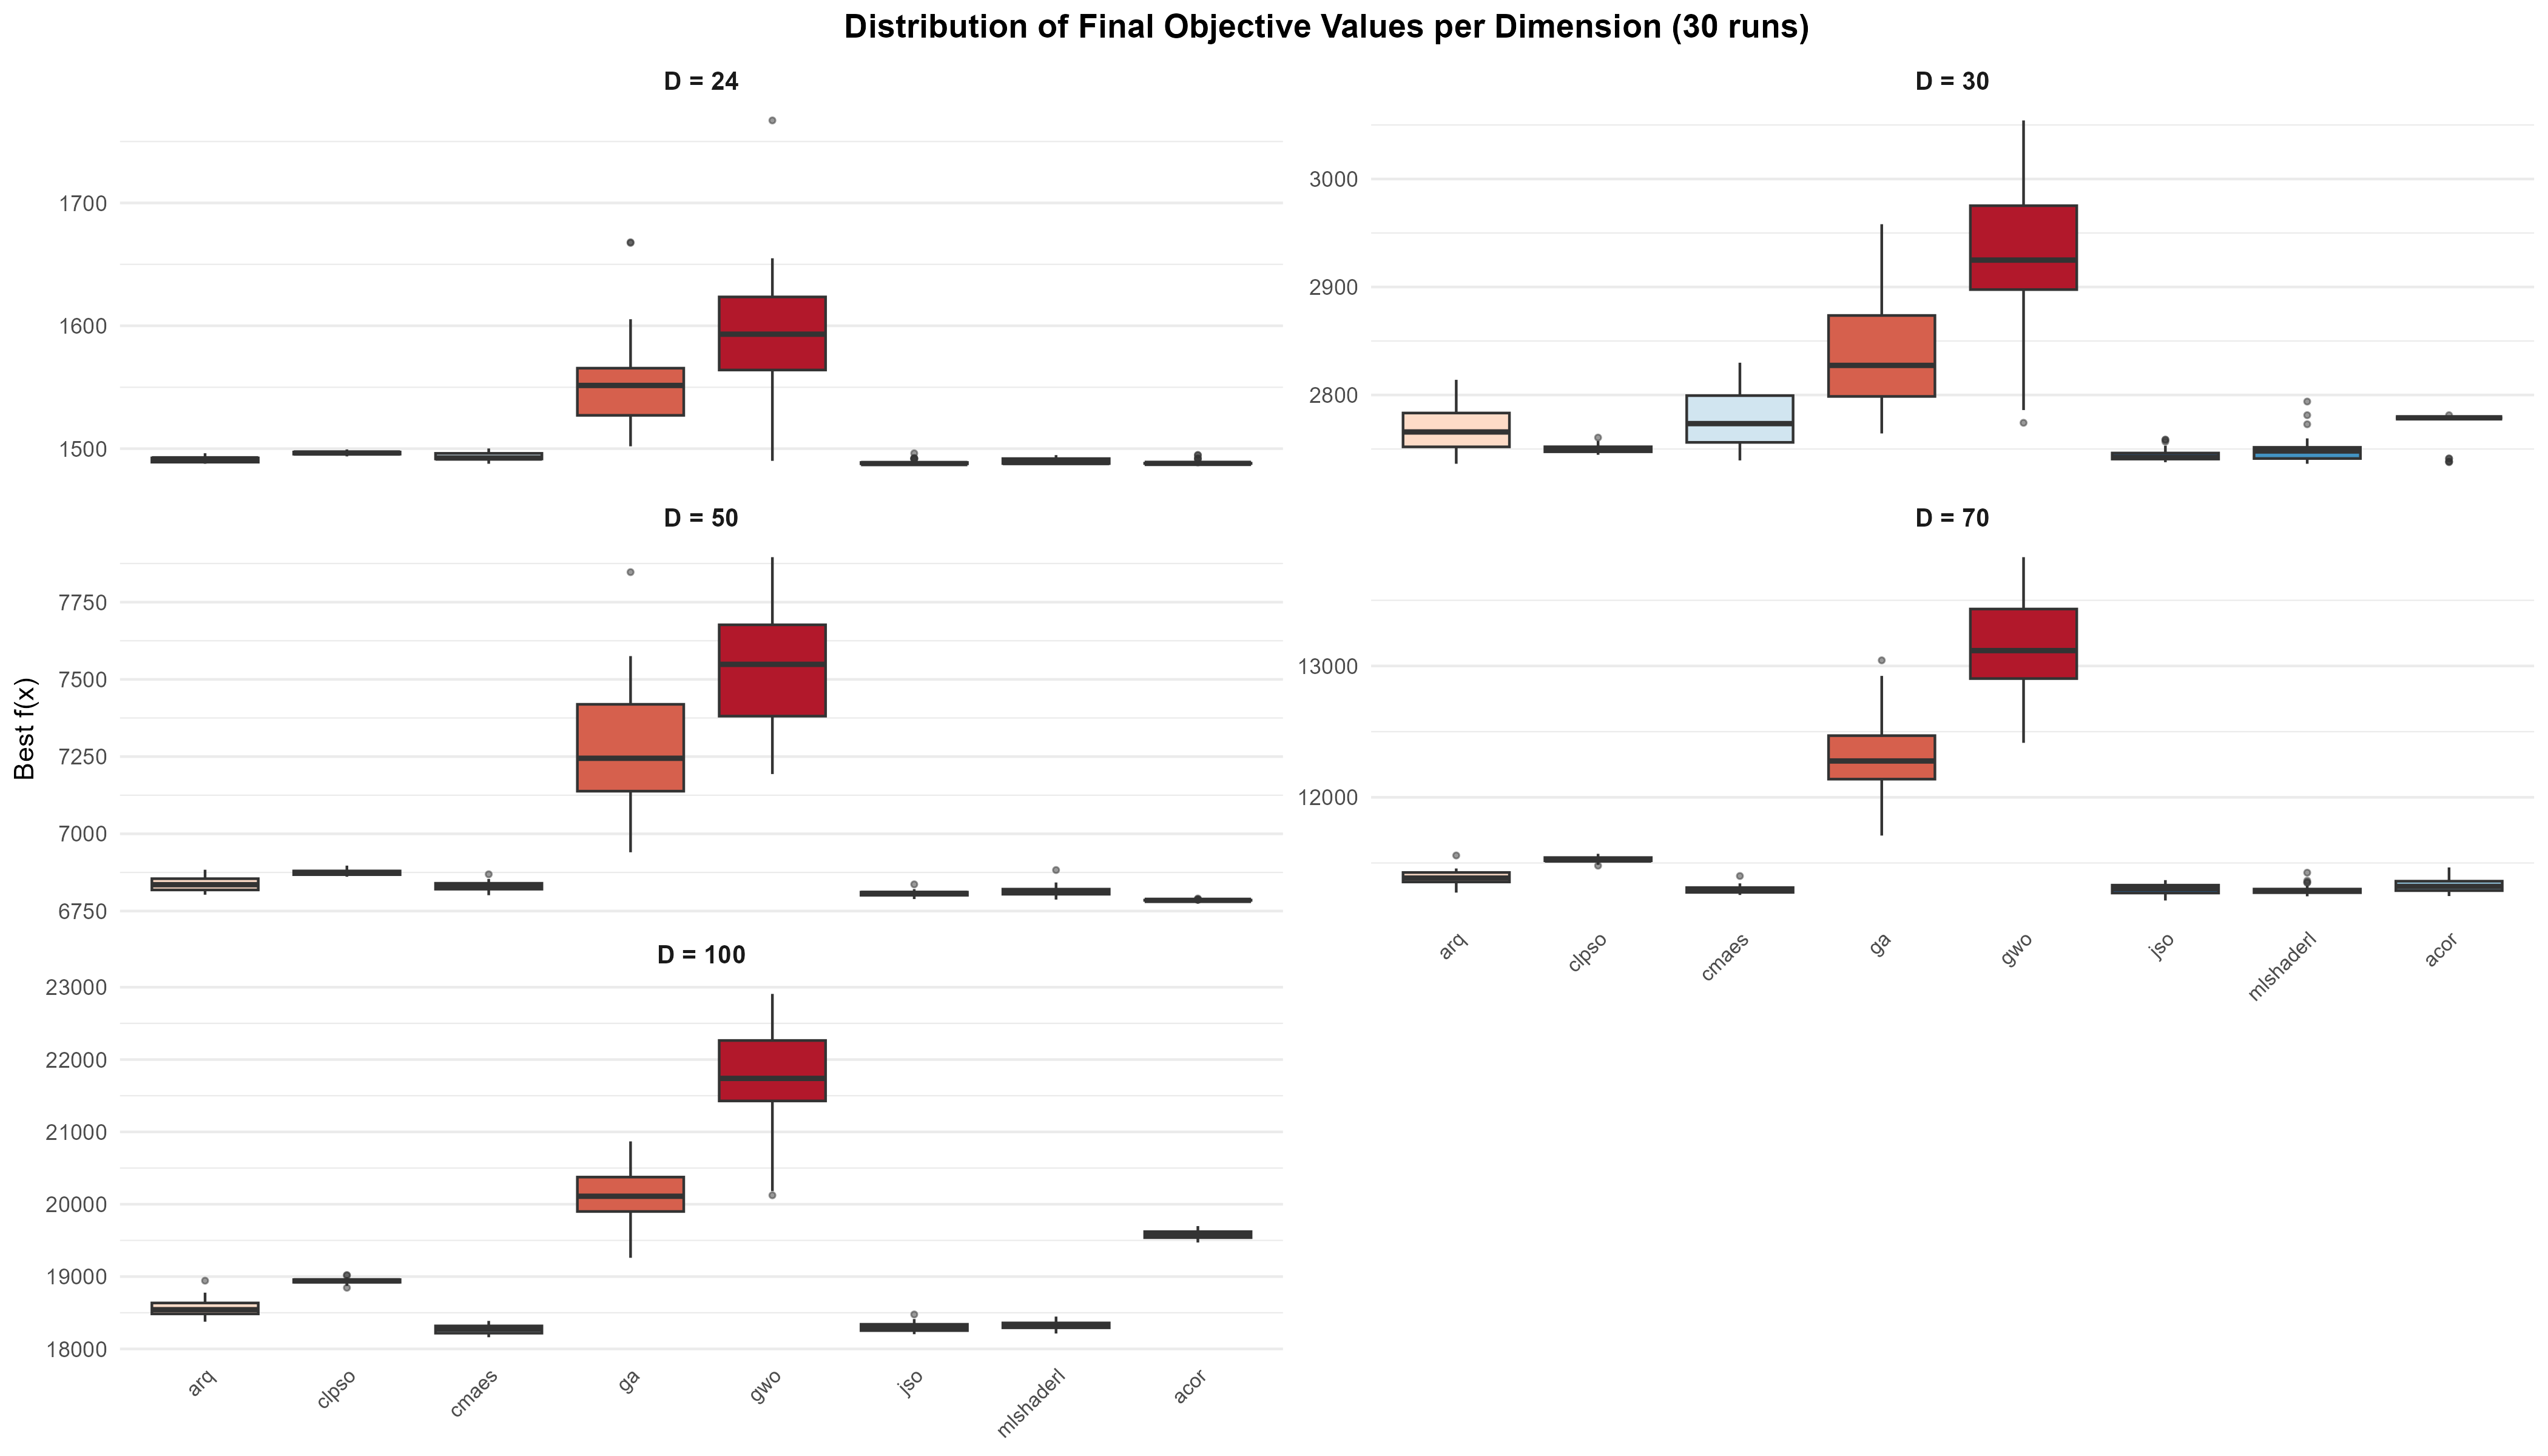
\includegraphics[scale=0.4]{boxplots}
\par\end{centering}
\caption{Distribution of final objective values per dimension for the full
benchmark formulation (30 independent runs)\label{fig:distribution}}
\end{figure}

Figure \ref{fig:distribution} complements the rank analysis by showing
the spread of final objective values. The tight interquartile ranges
of jso and mlshaderl at $D=24$ and $D=30$ contrast sharply with
the wide distributions of ga and gwo, which extend over hundreds of
objective-value units. At $D=70$ and $D=100$, all distributions
widen substantially, but the median values of jso and cmaes remain
consistently below those of the other methods, confirming the rank-based
findings.

\section{Discussion\label{sec:Discussion}}

Before discussing the experimental findings, it is useful to provide
a quantitative estimate of the landscape complexity induced by the
benchmark's primary difficulty mechanisms. The oscillatory efficiency
law $\eta_{i}(x)$ contains the term $sin{{}^2}(freq_{i}\cdot x_{i}+\varphi_{i})$,
which over the domain $x_{i}\in[0,80]$ completes approximately $freq_{i}\cdot80/\pi\approx0.22\cdot80/\pi\approx5.6$
half-cycles per variable at the default frequency. Each half-cycle
generates one local attractor in the efficiency landscape, so the
single-variable oscillatory structure alone produces approximately
5-6 local basins per stage. Since the efficiency also depends on the
neighbor-coupled load $N_{i}$ through the second sinusoidal term,
and since the storage state $S_{i}$ propagates effects from all preceding
stages, the number of combinatorially distinct local configurations
grows multiplicatively with D. A conservative lower bound on the number
of local attractors in the full problem is therefore on the order
of $5^{D}$, yielding approximately $5^{24}\approx6\times10^{16}$
at $D=24$ and $5^{50}\approx9\times10^{34}$ at $D=50$. While not
all of these correspond to true local minima of the composite objective
many are eliminated or merged by the smoothness, budget, and deficit
penalties this estimate explains why even sophisticated population-based
methods with typical population sizes of 100-500 individuals cannot
exhaustively cover the basin structure at moderate dimensions. The
recursive storage propagation further compounds this difficulty by
introducing a sequential dependency chain of length D: a perturbation
at stage i can alter the storage states $S_{i+1},...,S_{D}$ and thereby
shift the effective landscape seen by all subsequent variables. This
path dependence means that the effective dimensionality of the problem,
in terms of the number of coupled decisions that must be simultaneously
correct, is closer to $D{{}^2}$ than to $D$, consistent with the
empirical observation that solver success rates collapse between $D=30$
and $D=50$ rather than scaling smoothly with dimension.

The most salient observation across all five dimensions of the full
benchmark is the consistent superiority of jso and mlshaderl over
the remaining six methods. This outcome is not incidental. The method
jso employs a self-adaptive differential evolution strategy with weighted
mutation and crossover operators that balances exploration and exploitation
effectively in landscapes with moderate ruggedness. The method mlshaderl
relies on a historical archive mechanism that provides implicit memory
of previously explored regions and allows the search distribution
to contract toward promising basins without premature commitment.
In a landscape characterized by recursive state dependence, repeated
local oscillatory structure, and multiplicative coupling between stages,
these capabilities are precisely what distinguish reliable convergence
from stagnation. By contrast, methods such as ga and gwo, which rely
on simpler population recombination or swarm attraction heuristics,
consistently fail to maintain sufficient diversity in the presence
of the benchmark's multiple deceptive attractors, as evidenced by
their large standard deviations and their stable positioning at Friedman
ranks 7-8 across all dimensions. The dimension-scaling behavior observed
in the full formulation is consistent with the combinatorial growth
of non-separable interactions: the recursive storage propagation links
the effective landscape seen by variable $x_{i}$\LyXZeroWidthSpace{}
to decisions made at all preceding stages $x1,\ldots,x_{i-1}$\LyXZeroWidthSpace ,
creating an effective dependency chain whose length grows linearly
with $D$. As $D$ increases, the probability that a randomly initialized
trajectory can locate and remain in the correct basin across all stages
simultaneously diminishes rapidly, making global search substantially
harder than dimension alone would suggest for a separable or smoothly
non-separable problem.

The ablation protocol reveals a clear hierarchy of mechanism importance
that is both informative and practically useful. The oscillatory efficiency
mechanism emerges as the single most consequential source of landscape
ruggedness: its removal enables multiple solvers to achieve success
rates near or at 100\% even at $D=50$, a result that is unattainable
in the full formulation at that dimension. This finding has a clear
structural interpretation: the oscillatory modulation of $\eta_{i}(x)$,
which depends on both the local decision $x_{i}$ and the neighbor-coupled
load $N_{i}$\LyXZeroWidthSpace , introduces a dense lattice of local
attractors that are energetically competitive with the global basin.
In the absence of this mechanism, the residual landscape is sufficiently
smooth to permit gradient-like local improvement strategies to succeed
over repeated restarts. The recursive storage propagation and threshold
drainage mechanisms occupy the second tier, each contributing meaningful
but less dramatic difficulty that primarily affects the intermediate-dimensional
regime ($D=30-50$). The multiplicative yield aggregation, neighbor
coupling, and preferred-window regularization contribute more modestly,
with their effects becoming largely indistinguishable from the baseline
difficulty at high dimensions. Crucially, no single ablation restores
the problem to the triviality of the fully simplified variant, confirming
that the benchmark's difficulty is genuinely multi-mechanism in character.

The proposed benchmark addresses a recognized gap at the intersection
of two research communities. Within continuous global optimization,
the dominant benchmark suites including the CEC and BBOB families
are composed primarily of synthetic analytical functions whose difficulty
is controlled through transformation, rotation, and shifting, but
which lack the semantic interpretability and state-dependent coupling
of physically motivated problems. Within agricultural water management
and irrigation scheduling, the available simulation-optimization frameworks
are calibrated to specific field conditions and crop models and are
therefore neither self-contained nor designed to be algorithmically
difficult per se. The present benchmark occupies a complementary position:
it is analytically self-contained and fully deterministic, requires
no external data, exhibits a rich and verifiable difficulty structure
through the ablation protocol, and retains an agronomic interpretation
that makes its components meaningful beyond pure algorithmic testing.
The comparative evaluation against four classical benchmarks in Section
\ref{subsec:otherProblems} confirms quantitatively that the proposed
problem is substantially harder than Ackley, Rastrigin, Rosenbrock,
and Schwefel at the same dimensions, due to its simultaneous combination
of oscillatory ruggedness, non-separable coupling, deceptive global
structure, and stateful path dependence features that the classical
functions present only in isolation. The deliberate absence of a known
closed-form global optimum further distinguishes it from classical
synthetic benchmarks, making it a genuine black-box problem for which
algorithmic progress can only be measured empirically.

Although the proposed benchmark is not a calibrated digital twin of
any specific field or crop system, the experimental findings carry
implications that are transferable to the design of optimization-based
irrigation decision-support tools. The ablation study demonstrates
that temporal state coupling represented here by the recursive storage
mechanism and nonlinear efficiency losses are the two features that
most severely degrade optimizer performance. In practical irrigation
scheduling, these correspond precisely to the soil moisture carryover
between irrigation events and to the nonlinear relationship between
applied water and effectively delivered water, both of which are well-documented
challenges in field-level water management \citep{Allen,Linker,Zhao}.
The finding that archive-based and distribution-estimation methods
(jso, mlshaderl) substantially outperform simpler population-based
heuristics (ga, gwo) suggests that optimization tools deployed for
real irrigation scheduling should prioritize algorithms with adaptive
memory mechanisms capable of handling sequential dependencies, rather
than relying on general-purpose metaheuristics without such capabilities.
Furthermore, the parameter sensitivity analysis in Section \ref{subsec:sensitivity}
shows that the benchmark's difficulty is primarily controlled by a
small number of coefficients, most notably the oscillatory efficiency
amplitude. This means that practitioners wishing to use the benchmark
as a testbed for irrigation-oriented optimization tools can tune its
difficulty to match the complexity level of their target application
without altering the overall problem structure.

\section{Conclusions\label{sec:conclusions}}

This article has introduced a new continuous global optimization benchmark
derived from the semantics of weather-coupled irrigation scheduling.
The benchmark is formulated as a deterministic, box-constrained minimization
problem in which the objective function integrates a recursive soil-water
storage state, an oscillatory irrigation efficiency law, a multiplicative
seasonal yield factor, neighbor-coupled hydraulic penalties, threshold-triggered
drainage losses, and a deceptive preferred-window regularization term.
The problem is analytically self-contained: all exogenous weather
and crop profiles are generated from the normalized stage coordinate,
requiring no external datasets. Recommended problem dimensions span
from $D=24$ to $D=100$, with the transition from moderate to high
dimensionality producing a substantial and predictable increase in
landscape difficulty.

The experimental study, conducted over 30 independent runs of eight
established continuous optimizers across all recommended dimensions
and eight problem variants, yields three principal conclusions. First,
the full benchmark presents a genuinely multi-mechanism difficulty
that no single state-of-the-art solver reliably resolves at $D\ge50$:
even the best-performing method, jso (average Friedman rank 2.16),
achieves success rates of only 3\% at the highest dimensions tested.
Second, the ablation study identifies oscillatory efficiency modulation
as the dominant source of landscape ruggedness, with recursive storage
propagation and threshold drainage as the second tier of difficulty
mechanisms, together, these components account for the majority of
the difficulty gap between the full and the simplified formulations.
Third, the fully simplified variant, in which all embedded difficulty
mechanisms are disabled, is solved to optimality by most methods across
all dimensions, confirming that the observed difficulty in the full
formulation is structural rather than numerical in origin. The statistical
validation through Friedman and pairwise Wilcoxon tests confirms these
findings with $p$-values below $10^{-28}$at all dimensions. These
results collectively validate the proposed benchmark as a meaningful
and scalable tool for studying continuous optimization algorithms
on non-separable, stateful, and rugged landscapes with a clear agronomic
interpretation.

From a practical standpoint, the proposed benchmark offers the optimization
community a ready-to-use, computationally lightweight test problem
whose difficulty can be continuously adjusted through the oscillatory
efficiency amplitude and the resonance penalty weight, as demonstrated
by the sensitivity analysis in Section \ref{subsec:sensitivity}.
Its agronomic semantics also make it suitable as an educational or
demonstrative tool for illustrating how competing operational objectives
interact in seasonal resource-allocation problems. Several directions
for future work are identified. First, the evaluation of gradient-based
solvers, surrogate-assisted methods, and reinforcement-learning-based
optimizers on the benchmark would broaden the algorithmic coverage
beyond the population-based methods considered here. Second, a multi-objective
extension that separately optimizes water cost and seasonal yield,
rather than combining them in a single scalar objective, would enable
the study of Pareto-front structure under coupled weather-dependent
dynamics. Third, a stochastic variant in which the weather profiles
are drawn from parameterized distributions rather than fixed trigonometric
functions would allow the investigation of robust and risk-aware optimization
strategies. Fourth, a dynamic extension in which decisions are made
sequentially with partial observations of the storage state between
stages would transform the benchmark into a sequential decision problem
amenable to reinforcement learning and model predictive control. Finally,
future work could apply established exploratory landscape analysis
features such as fitness distance correlation, information content,
and gradient homogeneity measures  to the full and ablated formulations
across all recommended dimensions, providing a data-driven characterization
of how each difficulty mechanism shapes the search landscape.

\appendixtitles{no}

\begin{adjustwidth}{-\extralength}{0cm}{}

\begin{thebibliography}{999}
\bibitem{Rios}Rios, L. M., \& Sahinidis, N. V. (2013). Derivative-free
optimization: A review of algorithms and comparison of software implementations.
Journal of Global Optimization, 56(3), 1247-1293. https://doi.org/10.1007/s10898-012-9951-y

\bibitem{Sharma}Sharma, P., \& Raju, S. (2024). Metaheuristic optimization
algorithms: a comprehensive overview and classification of benchmark
test functions. Soft Computing, 28, 3123-3186. https://doi.org/10.1007/s00500-023-09276-5

\bibitem{Mohamed}Mohamed, A. W., Sallam, K. M., Agrawal, P., Hadi,
A. A., \& Mohamed, A. K. (2023). Evaluating the performance of meta-heuristic
algorithms on CEC 2021 benchmark problems. Neural Computing and Applications,
35, 1493-1517. https://doi.org/10.1007/s00521-022-07788-z

\bibitem{Naser}Naser, M. Z., Al-Bashiti, M. K., Tapeh, A. T. G.,
Naser, A., Kodur, V., Hawileh, R., Abdalla, J., Khodadadi, N., Gandomi,
A. H., \& Eslamlou, A. D. (2025). A Review of Benchmark and Test Functions
for Global Optimization Algorithms and Metaheuristics. Wiley Interdisciplinary
Reviews: Computational Statistics, 17(2), e70028. https://doi.org/10.1002/wics.70028

\bibitem{Kudela}Kudela, J. (2022). A critical problem in benchmarking
and analysis of evolutionary computation methods. Nature Machine Intelligence,
4, 1238-1245. https://doi.org/10.1038/s42256-022-00579-0

\bibitem{Liang-1}Liang, J. J., Qu, B. Y., \& Suganthan, P. N. (2013).
Problem definitions and evaluation criteria for the CEC 2014 special
session and competition on single objective real-parameter numerical
optimization. Technical Report 201311, Computational Intelligence
Laboratory, Zhengzhou University, China.

\bibitem{Hansen-1}Hansen, N., Finck, S., Ros, R., \& Auger, A. (2009).
Real-parameter black-box optimization benchmarking 2009: Noiseless
functions definitions. Research Report RR-6829, INRIA.

\bibitem{Awad}Awad, N. H., Ali, M. Z., Liang, J. J., Qu, B. Y., \&
Suganthan, P. N. (2016). Problem definitions and evaluation criteria
for the CEC 2017 special session and competition on single objective
real-parameter numerical optimization. Technical Report, Nanyang Technological
University, Singapore.

\bibitem{Varelas}Varelas, K., Ait El Hara, O., Brockhoff, D., Hansen,
N., Nguyen, D. M., Tušar, T., \& Auger, A. (2020). Benchmarking large-scale
continuous optimizers: The bbob-largescale testbed, a COCO software
guide and beyond. Applied Soft Computing, 97, 106737. https://doi.org/10.1016/j.asoc.2020.106737

\bibitem{Jamil}Jamil, M., \& Yang, X.-S. (2013). A literature survey
of benchmark functions for global optimisation problems. International
Journal of Mathematical Modelling and Numerical Optimisation, 4(2),
150-194. https://doi.org/10.1504/IJMMNO.2013.055204

\bibitem{Piotrowski-1}Piotrowski, A. P., Napiorkowski, J. J., \&
Piotrowska, A. E. (2024). Metaheuristics should be tested on large
benchmark sets with various numbers of function evaluations. Swarm
and Evolutionary Computation, 90, 101680. https://doi.org/10.1016/j.swevo.2024.101680

\bibitem{Das}Das, S., \& Suganthan, P. N. (2010). Problem definitions
and evaluation criteria for CEC 2011 competition on testing evolutionary
algorithms on real world optimization problems. Technical Report,
Jadavpur University, India.

\bibitem{Li}Li, Z., Zhou, Y., Zhang, S., Song, J., \& Li, X. (2023).
A large-scale continuous optimization benchmark suite with versatile
coupled heterogeneous modules. Swarm and Evolutionary Computation,
79, 101280. https://doi.org/10.1016/j.swevo.2023.101280

\bibitem{Jamal}Jamal, A., Linker, R., \& Housh, M. (2023). Real-time
irrigation scheduling based on weather forecasts, field observations,
and human-machine interactions. Water Resources Research, 59(12),
e2023WR035810. https://doi.org/10.1029/2023WR035810

\bibitem{Allen}Allen, R. G., Pereira, L. S., Raes, D., \& Smith,
M. (2025). Crop evapotranspiration: Guidelines for computing crop
water requirements (2nd rev. ed.). FAO Irrigation and Drainage Paper
56. Food and Agriculture Organization of the United Nations. https://doi.org/10.4060/cd6621en

\bibitem{Doorenbos}Doorenbos, J., \& Kassam, A. H. (1979). Yield
response to water. Irrigation and Drainage Paper 33. Food and Agriculture
Organization of the United Nations. https://doi.org/10.1016/B978-0-08-025675-7.50021-2

\bibitem{Wang}Wang, D., \& Cai, X. (2009). Irrigation scheduling
- Role of weather forecasting and farmers' behavior. Journal of Water
Resources Planning and Management, 135(5), 364-372. https://doi.org/10.1061/(ASCE)0733-9496(2009)135:5(364)

\bibitem{Linker}Linker, R., \& Kisekka, I. (2023). Model-based simulation-optimization
of irrigation scheduling - A field evaluation with processing tomatoes.
Smart Agricultural Technology, 4, 100234. https://doi.org/10.1016/j.atech.2023.100234

\bibitem{Li-1}Li, X., Zhang, J., Cai, X., Huo, Z., \& Zhang, C. (2023).
Simulation-optimization based real-time irrigation scheduling: A human-machine
interactive method enhanced by data assimilation. Agricultural Water
Management, 276, 108059. https://doi.org/10.1016/j.agwat.2022.108059 

\bibitem{Zhao}Zhao, Y., Li, G., Li, S., Luo, Y., \& Bai, Y. (2024).
A review on the optimization of irrigation schedules for farmlands
based on a simulation-optimization model. Water, 16(17), 2545. https://doi.org/10.3390/w16172545

\bibitem{Charilogis}Charilogis, V., Tsoulos, I. G., Gianni, A. M.,
\& Tsalikakis, D. (2025). ARQ: A cohesive optimization design for
stable performance on noisy landscapes. Applied Sciences, 15(22),
12180. doi:10.3390/app152212180.

\bibitem{Liang}Liang, J. J., Qin, A. K., Suganthan, P. N., \& Baskar,
S. (2006). Comprehensive learning particle swarm optimizer for global
optimization of multimodal functions. IEEE Transactions on Evolutionary
Computation, 10(3), 281-295. doi:10.1109/TEVC.2005.857610.

\bibitem{Hansen}Hansen, N., \& Ostermeier, A. (2001). Completely
derandomized self-adaptation in evolution strategies. Evolutionary
Computation, 9(2), 159-195. https://doi.org/10.1162/106365601750190398

\bibitem{Holland}Holland, J. H. (1992). Adaptation in natural and
artificial systems: An introductory analysis with applications to
biology, control, and artificial intelligence (2nd ed.). MIT Press.
https://doi.org/10.7551/mitpress/1090.001.0001

\bibitem{Mirjalili}Mirjalili, S., Mirjalili, S. M., \& Lewis, A.
(2014). Grey Wolf Optimizer. Advances in Engineering Software, 69,
46-61. https://doi.org/10.1016/j.advengsoft.2013.12.007

\bibitem{Brest}Brest, J., Maučec, M. S., \& Bošković, B. (2017).
Single objective real-parameter optimization: Algorithm jSO. In 2017
IEEE Congress on Evolutionary Computation (CEC) (pp. 1311-1318). doi:10.1109/CEC.2017.7969456

\bibitem{Chauhan}Chauhan, D., Trivedi, A., \& Shivani. (2024). A
multi-operator ensemble LSHADE with restart and local search mechanisms
for single-objective optimization. arXiv. doi:10.48550/arXiv.2409.15994

\bibitem{Socha}Socha, K., \& Dorigo, M. (2008). Ant colony optimization
for continuous domains. European Journal of Operational Research,
185(3), 1155-1173. https://doi.org/10.1016/j.ejor.2006.06.046

\bibitem[(1987)]{Ackley}Ackley, D. H. (1987). A Connectionist Machine
for Genetic Hillclimbing. Kluwer Academic Publishers.

\bibitem[(1974)]{Rastrigin}Rastrigin, L. A. (1974). Systems of Extremal
Control. Nauka, Moscow. (In Russian)

\bibitem[(1960)]{Rosenbrock}Rosenbrock, H. H. (1960). An automatic
method for finding the greatest or least value of a function. The
Computer Journal, 3(3), 175-184. https://doi.org/10.1093/comjnl/3.3.175

\bibitem[(1981)]{Schwefel}Schwefel, H.-P. (1981). Numerical Optimization
of Computer Models. John Wiley \& Sons.

\bibitem{Piotrowski}Piotrowski, A. P., Napiorkowski, J. J., \& Piotrowska,
A. E. (2023). Choice of benchmark optimization problems does matter.
Swarm and Evolutionary Computation, 83, 101378.

\bibitem{Kumar}Kumar, A., Misra, R. K., \& Singh, D. (2024). A comprehensive
survey of benchmark functions for evolutionary and swarm intelligence
algorithms. Knowledge-Based Systems, 283, 111170.

\end{thebibliography}

\end{adjustwidth}{}
\end{document}
